\documentclass[11pt,a4paper]{article}

\usepackage[utf8]{inputenc}
\usepackage[T1]{fontenc}
\usepackage{lmodern}
\usepackage[margin=0.95in]{geometry}
\usepackage{amsmath,amssymb,amsfonts,amsthm}
\usepackage{booktabs}
\usepackage{array}
\usepackage{graphicx}
\usepackage{xcolor}
\usepackage{tikz}
\usetikzlibrary{arrows.meta,positioning,fit,calc}
\usepackage{hyperref}
\usepackage{listings}
\usepackage{enumitem}
\usepackage{fancyhdr}
\emergencystretch=3em
\sloppy

\hypersetup{
    colorlinks=true,
    linkcolor=blue!70!black,
    citecolor=green!50!black,
    urlcolor=blue!80!black,
    pdftitle={Project HiveMind: A System Design for Decentralized Sparse Mixture-of-Experts Training with DiLoCo-Style Outer Optimization on 8 GB Consumer GPUs},
    pdfauthor={Xavier Callens and Project HiveMind Open-Source Swarm Collective}
}

\newtheorem{theorem}{Theorem}[section]
\newtheorem{lemma}[theorem]{Lemma}
\newtheorem{proposition}[theorem]{Proposition}
\newtheorem{invariant}[theorem]{Invariant}
\newtheorem{definition}[theorem]{Definition}

\definecolor{codebg}{RGB}{246,248,250}
\definecolor{codeframe}{RGB}{208,215,222}
\definecolor{leanblue}{RGB}{0,92,197}
\definecolor{leankw}{RGB}{215,58,73}

\lstdefinelanguage{Lean4}{
  keywords={namespace, end, def, theorem, lemma, by, unfold, omega, decide, simp, where, if, then, else, import, open, constructor, exact, have, rw},
  keywordstyle=\color{leankw}\bfseries,
  sensitive=true,
  comment=[l]{--},
  morecomment=[s]{/-}{-/},
  commentstyle=\color{gray}\itshape,
  basicstyle=\ttfamily\footnotesize,
  backgroundcolor=\color{codebg},
  frame=single,
  rulecolor=\color{codeframe},
  breaklines=true,
  showstringspaces=false
}

\IfFileExists{zenodo_doi.tex}{\newcommand{\zenodoDOI}{10.5281/zenodo.23776302}
}{\newcommand{\zenodoDOI}{pending}}
\pagestyle{fancy}
\setlength{\headheight}{21pt}
\fancyhf{}
\lhead{\footnotesize \textbf{Project HiveMind v3.8.0} --- Decentralized Sparse MoE \& DiLoCo on 8\,GB GPUs: System Design, Experiments \& Proofs}
\rhead{\footnotesize \thepage}
\cfoot{\footnotesize Preprint (not peer reviewed; scripted audits only) $\cdot$ Zenodo DOI of the deposited version (v3.7.1): \zenodoDOI{} $\cdot$ \url{https://github.com/xaviercallens/HiveMind}}

\title{\vspace{-1.3cm}\textbf{Project HiveMind: A System Design for Decentralized Sparse Mixture-of-Experts Training with DiLoCo-Style Outer Optimization on 8\,GB Consumer GPUs}\\[0.35em]
\large \textit{Integration of Low-Communication Training Methods, Controlled Experimental Evaluations, and Lean 4 Bookkeeping Lemmas}}

\author{
  \textbf{Xavier Callens}\thanks{Project HiveMind (\texttt{callensxavier@gmail.com}). Code and all artifacts referenced in this paper: \url{https://github.com/xaviercallens/HiveMind}. The project is non-commercial; contributors receive no payment.} \\
  Project HiveMind Open-Source Contributors
}

\date{October 24, 2026 --- Version 3.8.0 (re-based onto v3.7.2: adds the pre-registered results of the 23/24 October 2026 T4 campaign, namely E10b (invalid), E11 (Qwen2.5-Coder-7B row invalid and withdrawn), E12 on the T4 and E13 to E16 with the GWAYA-Lite deployment; v3.7.2: independent Lean gate re-run at 128 theorems; E12 replay-divergence pilot complete: bf16 precision class diverges beyond the tampered control; revised after an external review of v3.5.0, response in \texttt{paper/review/}; pre-registered research program; E5-toy, E5-het and E10 three-seed experiments; RDA as an outer-LR multiplier, machine-checked over $\mathbb{R}$; E8 two-host internet pilot; 120 Lean 4 lemmas + 3 Mathlib theorems)}

\begin{document}

\maketitle

\begin{abstract}
\noindent
Training and serving frontier Large Language Models (LLMs) are increasingly monopolized by hyperscale datacenters due to two fundamental systems bottlenecks: the \textbf{VRAM Wall} (a single 8\,GB--12\,GB consumer GPU cannot hold a 70B+ dense model or its FP32 AdamW optimizer states) and the \textbf{Bandwidth Wall} (standard synchronous All-Reduce Distributed Data Parallelism saturates 10--50\,Mbps residential internet links instantly). Yet the global PC gaming and open-source developer community possesses millions of idle NVIDIA RTX 20/30/40-series, AMD ROCm, and Apple Metal GPUs alongside terabytes of NVMe flash storage.

We describe \textbf{Project HiveMind}, an open-source decentralized training and inference system, and report what has and has not yet been validated. The system combines \textbf{Branch-Train-Mix (BTM) sparse MoE upcycling}, \textbf{weight-tied looped recurrence}, and \textbf{DiLoCo-style outer optimization}, with an emphasis on fitting a strict 8\,GB GPU memory budget. Workers stream open-weight backbones (\texttt{Qwen2.5}) into 4-bit NF4 and train QLoRA adapters; outer pseudo-gradients can be compressed with a DCT + 2-bit centroid scheme adapted from DeMo~\cite{peng2024demo} and SparseLoCo~\cite{sarfi2025sparseloco}; the outer optimizer supports a CPU-resident flat-bucket state (after \texttt{prime-diloco}~\cite{jaghouar2024opendiloco}) and the staleness gate of CGAD~\cite{shah2026cgad}; converged branches are upcycled into a sparse MoE with optional Iso-CTS~\cite{marczak2025iso} or TSV~\cite{gargiulo2024tsv} attention merging and FoMoE-style partial expert replication~\cite{sani2026fomoe}.

\textbf{Empirical and formal evaluation.} We evaluate the system at three levels, separating verified properties from open multi-node questions: (i) Ten \emph{unit-level implementation checks} (\texttt{H1}--\texttt{H10}, \texttt{artifacts/architecture\_hypothesis\_verification\_report.json}) verify that each component satisfies its mathematical specification on controlled tensors, including non-trivial fixed-point halting ($\epsilon_{\text{fp}} = 0.65 \Rightarrow 3.05/4.0$ mean recurrent steps) and single-round vs.\ multi-step EF21 error-feedback conservation; an eleventh check (\texttt{H11}, \texttt{artifacts/decoupled\_diloco\_quorum\_check.json}) covers a Decoupled DiLoCo syncer~\cite{douillard2026decoupled} with minimum quorum, adaptive grace window and token-weighted Radial-Directional Averaging, which restores the common outer-gradient norm that direct averaging shrinks by $1/\sqrt{M}$ ($2.83\times$ at $M=8$). (ii) Four \emph{controlled multi-regime experimental studies} (\texttt{E1}--\texttt{E4}, \texttt{artifacts/paper\_v3\_experiments\_report.json}, Figures~\ref{fig:e1_convergence}--\ref{fig:e4_vram_fomoe}) measure held-out generalization across five synchronization regimes (showing that DeMo 2D-DCT + SparseLoCo 2-bit + EF21 achieves a \textbf{0.052\%} held-out loss gap vs.\ uncompressed FP32 DiLoCo while cutting outer wire traffic by \textbf{12.49$\times$} and \textbf{99.9$\times$} vs.\ synchronous DDP, and that \texttt{MuLoCo} 5-step Newton-Schulz inner preconditioning slightly improves compressed held-out perplexity), outer convergence under severe straggler bursts ($\tau_w \ge 36$, where \texttt{PA-CGAD} reduces terminal MSE by \textbf{11.6$\times$} relative to un-gated outer AdamW), fixed-point halting trade-offs across $\epsilon_{\text{fp}} \in [0.0, 1.10]$, and singular value spectra under \texttt{Iso-CTS} and \texttt{TSV} merging. (iii) A single-GPU proof of concept on an 8\,GB NVIDIA RTX 2070 with \texttt{Qwen2.5-0.5B} trains four domain branches and upcycles them into a 4-expert top-2 MoE within \textbf{1{,}509.5\,MB} peak VRAM, accompanied by \textbf{120} zero-\texttt{sorry} Lean 4 arithmetic and hypothesis-necessity lemmas (\texttt{lean4/HiveMindSpec.lean}). \textbf{Research program.} Because all experiments so far are single-host and single-seed, Section~\ref{sec:research} turns the design into a testable thesis: the loss gap between a volunteer WAN swarm and a single-host run at matched tokens should decompose into the replica-count penalty of the DiLoCo scaling law plus a bounded ``volunteer tax''. It states eight research questions, the prediction each makes, the observation that would refute it, and five pre-registered experiments (E5--E9, three seeds, positive, negative and matched-random controls) that decide them. Section~\ref{sec:limitations} details remaining multi-host WAN limitations. \textbf{Update in v3.8.0.} Three further pre-registered experiments were run on one Tesla T4 (Section~\ref{sec:status380}): a lattice codec for outer deltas at 0.5B scale (E10b, invalid by its registered rule), lattice codecs for the KV cache on three models (E11: the registered prediction was refuted on the two valid models, the Qwen2.5-Coder-7B row is invalid because its negative control failed and its verdicts are withdrawn, and the KV ring stays on FP8), and the replay divergence of the spot-check across hardware (E12 on the T4, exact on the same GPU, above the tolerance between a GPU and a CPU, complementing the CPU pilot of Section~\ref{sec:e12}). Refuted and invalid outcomes are reported as such. A second batch of pre-registered experiments (Sections~\ref{sec:e13}--\ref{sec:e16}) adds: a swarm simulation on one GPU with real localhost HTTP between workers (E13: the protocol reproduces the synchronous baseline bit for bit, the codec cuts the upload to $9.1\,\%$ of the raw bytes, and the registered viability prediction for the all-mechanisms-on swarm at $K=\lceil M/2\rceil$ is \emph{refuted} on a dense and on a pretrained mixture-of-experts model, the loss being attributed to the quorum); a fair-quorum and a deferred-carry policy (E14: supported on the dense model, inconclusive on the MoE); a gate-selected rejection-sampling fine-tuning of a 1.5B coding model under an enforced 7.5\,GiB cap (E15: the inference-time gate lifts MBPP pass@1 from $65.8\,\%$ to $72.8\,\%$, the fine-tuning does not detectably); and the measured VRAM, speed and accuracy of three quantised coding tiers on a Tesla T4 with a deployed loopback assistant (E16, GWAYA-Lite). Refuted, inconclusive and invalid outcomes are reported as such, and no peer review of record has taken place.

\end{abstract}

\vspace{0.3em}
\noindent\textbf{Keywords:} Decentralized AI $\cdot$ Pre-registered Experiments $\cdot$ Sparse Mixture-of-Experts (MoE) $\cdot$ DiLoCo \& OpenDiLoCo $\cdot$ FoMoE $\cdot$ Looped Transformers $\cdot$ DeMo DCT \& SparseLoCo $\cdot$ MuLoCo Newton-Schulz $\cdot$ Byzantine Fault Tolerance $\cdot$ Lean 4

\tableofcontents
\newpage

% ============================================================================
\section{Introduction: Breaking the VRAM and Bandwidth Walls}
% ============================================================================

Modern frontier language models rely on massive parameter counts ($70\text{B} \text{ to } 1\text{T+}$) trained over tightly coupled InfiniBand or NVLink fabrics ($400\text{--}3,200\text{\,Gbps}$). Attempting to decentralize LLM training and inference across volunteer consumer gaming hardware---the modern equivalent of \texttt{SETI@home} \cite{anderson2002boinc} and \texttt{Folding@home}---confronts four structural barriers:

\begin{enumerate}[leftmargin=1.8em]
    \item \textbf{The Consumer VRAM Wall:} The median gaming GPU on the Steam Hardware Survey (e.g., NVIDIA RTX 2070, RTX 3060, RTX 4060) provides \textbf{8\,GB to 12\,GB of GDDR6 VRAM}. On Windows 10/11 under the WDDM display driver model, approximately $1.0\text{--}1.5\text{\,GB}$ is reserved by the operating system and desktop compositor, leaving a strict usable ceiling of $M_{\text{ceil}} \approx 6.5\text{\,GB}$ on an 8\,GB card. A dense 7B model in FP16 with FP32 master weights and AdamW first/second moments requires $>56\text{\,GB}$ of VRAM, causing immediate out-of-memory (OOM) failure.
    \item \textbf{The Residential WAN Bandwidth \& Straggler Wall:} Standard Distributed Data Parallel (DDP) training executes an All-Reduce over all gradients at every micro-step ($t = 1, 2, \dots$). Over residential fiber or cable connections ($10\text{--}50\text{\,Mbps}$ upload, $20\text{--}150\text{\,ms}$ RTT), synchronizing gigabytes of gradients per second is physically impossible. Even under Distributed Low-Communication (\texttt{DiLoCo}) \cite{douillard2023diloco} training, asynchronous WAN stragglers inject stale pseudo-gradients that corrupt outer momentum and inflate outer Adam second moments \cite{shah2026cgad}.
    \item \textbf{The Sparse MoE All-to-All \& PCIe Thrashing Wall:} Scaling model capacity via Mixture-of-Experts (MoE) \cite{fedus2022switch,sukhbaatar2024btm,charles2025scalingdiloco} traditionally requires either holding all $E$ experts in GPU VRAM (violating the 8\,GB ceiling when $E = 64\text{--}128$) or issuing synchronous token-level All-to-All RPCs and synchronous PCIe DMA loads that stall the GPU for $2\text{--}20\text{\,ms}$ per layer.
    \item \textbf{The Byzantine \& Gamer Preemption Threat:} Volunteer consumer nodes include unstable GPU overclocks, bit-flips, Sybil botnets, and adversarial gradient poisoners. Classic BOINC mitigates this via $2\times$ redundant workunit replication (wasting $50\%$ of cluster FLOPs), while gamers demand $<1.5\text{\,s}$ preemption latency whenever a game launches.
\end{enumerate}

\subsection{Architecture Overview \& Summary of Contributions}

\textbf{Project HiveMind} addresses these barriers with four design pillars (Sections 3--5), a next-generation \textbf{Hierarchical, Federated \& Looped Sparse MoE architecture} (Section 6), and a unified \textbf{Google DeepMind DiLoCo + Prime Intellect OpenDiLoCo outer-loop stack} (Section 7):

\begin{itemize}[leftmargin=1.8em]
    \item \textbf{Pillar 1 (Zero-Copy 4-Bit NF4 + MuLoCo-Preconditioned DiLoCo-QLoRA):} Meta-device skeleton initialization with streaming 4-bit NormalFloat (\texttt{NF4}) double quantization (\texttt{0\,B} CPU heap duplication) paired with inner-loop \textbf{5-step quintic Newton-Schulz LoRA gradient orthogonalization} (Muon~\cite{jordan2024muon}, as used inner-loop by MuLoCo~\cite{therien2025muloco,belilovsky2026inner}) and \textbf{EF21 error-feedback wire compression} \cite{richtarik2021ef21,sarfi2025sparseloco,peng2024demo}.
    \item \textbf{Pillar 2 (Byzantine Fault Tolerance Without $2\times$ Replication):} Deterministic CUDA execution (\texttt{CUBLAS\_WORKSPACE\_CONFIG=:4096:8}) with SHA-256 micro-checkpoints every $s=50$ steps enables 10\% random segment replay within $\epsilon \le 10^{-4}$ ($20\times$ fewer verification FLOPs than $2\times$ BOINC), paired with \textbf{Multi-Krum $2\sigma$ cosine filtering} \cite{blanchard2017krum} and \textbf{ZK-OPoI v4 position-bound batch Merkle verification}.
    \item \textbf{Pillar 3 \& Missing MoE Architecture (128-Expert 3-Tier Hierarchical MoE, \texttt{FoMoE}, \texttt{Skip-Attention} \& \texttt{LoopedExpertBackbone}):} We extend Branch-Train-Mix (BTM) \cite{sukhbaatar2024btm} with (i) a \textbf{3-Tier $4 \times 4 \times 8 = 128$-Expert Hierarchical Router} ($8.0\times$ gating FLOP reduction), (ii) \textbf{Federated Partial Expert Replication (\texttt{FoMoE})} \cite{sani2026fomoe} with \textbf{Ghost-Expert \texttt{Skip-Token}} local routing ($3.46\times$ WAN ring reduction, zero remote FFN RPCs), (iii) \textbf{\texttt{Skip-Attention} Speculative Prefetch + Cache-Aware Routing (\texttt{CAR})} \cite{merolla2025fomoe} (so far evaluated only in a synthetic unit check), (iv) \textbf{\texttt{Iso-CTS} \& \texttt{TSV} Subspace Attention Merging} \cite{marczak2025iso,horoi2026isoloco,gargiulo2024tsv}, and (v) a \textbf{Weight-Tied \texttt{LoopedExpertBackbone}} (\texttt{Prelude} $\to$ \texttt{RecurrentCore} $\times T \to$ \texttt{Coda}) \cite{loopedmoe2026,loopedfp2026} with per-token fixed-point convergence exit and truncated BPTT.
    \item \textbf{Next-Generation OpenDiLoCo \& Google DeepMind Outer-Loop Stack:} Building on Google DeepMind's \texttt{DiLoCo} \cite{douillard2023diloco}, asynchronous Local-SGD \cite{liu2024asynclocalsgd}, \texttt{Streaming DiLoCo} \cite{douillard2025streamingdiloco}, \texttt{Scaling Laws for DiLoCo} \cite{charles2025scalingdiloco}, and \texttt{Decoupled DiLoCo} \cite{douillard2026decoupled} with Prime Intellect's \texttt{OpenDiLoCo} / \texttt{prime-diloco} \cite{jaghouar2024opendiloco}, we implement a \textbf{Contiguous 1D CPU Flat-Bucket Outer State} (\texttt{0\,B} extra GPU VRAM), \textbf{Cosine-Gated Adam-Decay (\texttt{PA-CGAD})} \cite{shah2026cgad} with uniform staleness bias bound $\max_{\tau \ge 0} \tau \sigma(\tau) \le \frac{1}{e\alpha}$, \textbf{\texttt{DeMo} + \texttt{SparseLoCo} + \texttt{PULSELoCo}-style 2-bit DCT wire compression} \cite{peng2024demo,sarfi2025sparseloco,miahi2026pulseloco}, \textbf{\texttt{AutoLoCo}} \cite{he2026autoloco}, \textbf{\texttt{HeLoCo}} \cite{asif2026heloco}, and a \textbf{Decoupled DiLoCo quorum syncer} (minimum quorum $K$, adaptive grace window $\xi_{\text{grace}} \le \gamma\,\xi_{\text{slack}}$, token-weighted Radial-Directional Averaging; Section~\ref{sec:decoupled}).
    \item \textbf{Pre-registered research program (Section~\ref{sec:research}):} a thesis, eight falsifiable predictions with refutation criteria, a scaling-law prior, five pre-registered experiments with controls, and decision rules that say what each outcome changes in the system and in this paper.
    \item \textbf{Honest scope statement:} each pillar is implemented and unit-tested, but the end-to-end system has not yet been evaluated across multiple machines or against a data-parallel baseline (Section~\ref{sec:limitations}).
\end{itemize}

% ============================================================================
\begin{figure}[ht!]
\centering
\begin{tikzpicture}[font=\scriptsize, node distance=3mm and 2.5mm,
  box/.style={draw, rounded corners=1pt, align=center, inner sep=2pt, minimum height=5.5mm, fill=white, text width=29mm},
  frozen/.style={box, fill=gray!12}, train/.style={box, fill=blue!8}, net/.style={box, fill=orange!10}, sync/.style={box, fill=green!8},
  arr/.style={-{Stealth[length=1.6mm]}, thick}]
% ---------- panel (a): one worker inner step ----------
\node[frozen] (nf4) {NF4 base weights (frozen, 4-bit)\\zero-copy meta-device stream, \texttt{H1}};
\node[train, right=of nf4] (lora) {LoRA adapters (trainable)\\rank $r$, \texttt{DiLoCoInnerLoop}};
\node[box, right=of lora] (moe) {sparse MoE block\\3-tier router $\to$ resident experts\\\texttt{FoMoE}: ghost-routed tokens skipped};
\node[box, right=of moe] (loss) {loss, backward\\AdamW on adapters only};
\node[train, below=of loss] (inner) {$H$ inner steps};
\node[train, below=of moe] (delta) {pseudo-gradient\\$\Delta = \theta_{\text{start}} - \theta_{\text{end}}$};
\node[net, below=of lora] (comp) {compress: chunked DCT, 2-bit LUT\\$+$ EF21 residual carry (Thm.~107)};
\node[net, below=of nf4] (ship) {ship $\mathcal{C}(\Delta)$ + token count\\over QUIC/TURN};
\draw[arr] (nf4) -- (lora); \draw[arr] (lora) -- (moe); \draw[arr] (moe) -- (loss);
\draw[arr] (loss) -- (inner); \draw[arr] (inner) -- node[below, pos=0.25, xshift=1mm]{after $H$} (delta); \draw[arr] (delta) -- (comp); \draw[arr] (comp) -- (ship);
\draw[arr, dashed] (inner.east) -- ++(3mm,0) node[right, pos=1, yshift=3mm, align=left]{repeat\\$H$ times} |- (loss.east);
\node[fit=(nf4)(loss)(ship), draw, dashed, gray, inner sep=4pt, label={[gray, anchor=south west]north west:(a) one worker, $< 8$\,GB VRAM: budget checked by \texttt{H1}, \texttt{H4}, PoC}] {};
% ---------- panel (b): one outer-loop synchronisation ----------
\node[net, below=17mm of ship] (l1) {learner 1\\$\mathcal{C}(\Delta_1)$, tokens, arrival $t_1$};
\node[net, right=of l1] (l2) {learner 2 $\cdots$ learner $M$\\(stragglers arrive late or not at all)};
\node[sync, right=of l2] (quorum) {syncer: quorum $K \le M$\\adaptive grace window $\gamma\,\xi_{\text{slack}}$\\token weights (Thms.~117--120)};
\node[sync, right=of quorum] (merge) {merge admitted deltas\\RDA or direct (Prop.~\ref{prop:rda_multiplier})\\deferred deltas carried};
\node[sync, below=of merge] (gate) {staleness gate\\PA-CGAD $\sigma(\tau)$ (off when $K<M$)};
\node[sync, below=of quorum] (outer) {outer Nesterov on CPU\\flat bucket, 0\,B GPU (\texttt{H11})};
\node[net, below=of l2] (bcast) {broadcast fragments\\(Streaming DiLoCo schedule)};
\node[net, below=of l1] (back) {learners start next\\inner phase from $\theta^{(t+1)}$};
\draw[arr] (l1) -- (l2); \draw[arr] (l2) -- (quorum); \draw[arr] (quorum) -- (merge); \draw[arr] (merge) -- (gate); \draw[arr] (gate) -- (outer); \draw[arr] (outer) -- (bcast); \draw[arr] (bcast) -- (back);
\draw[arr, dashed] (back.north) -- node[right, pos=0.5]{round $t{+}1$} (l1.south);
\node[fit=(l1)(merge)(back), draw, dashed, gray, inner sep=4pt, label={[gray, anchor=south west]north west:(b) one outer round over the WAN: measured so far on two hosts (E8 pilot) and in single-host simulation (E1--E5)}] {};
\end{tikzpicture}
\caption{Architecture overview requested by the external review of v3.5.0. (a) One worker's inner step under the 8\,GB budget: frozen NF4 base, trainable LoRA adapters, a sparse MoE block whose non-resident (ghost) experts are skipped, $H$ inner steps, then the pseudo-gradient is DCT-compressed to 2 bits with error-feedback residual carry and shipped. (b) One outer round: learner deltas reach the CPU-resident syncer, a quorum of $K$ plus a grace window decides admission, admitted deltas are merged (RDA or direct), optionally gated by staleness, applied by the CPU flat-bucket Nesterov step and broadcast by fragments. Grey captions name the check or experiment that has actually exercised each panel.}
\label{fig:architecture}
\end{figure}

\section{Lean 4 Bookkeeping Lemmas: Scope and Limits}
% ============================================================================

We maintain a Lean 4 \cite{moura2021lean4} file of arithmetic and necessity lemmas that accompany the design (\texttt{lean4/HiveMindSpec.lean}, compiled with \texttt{leanprover/lean4:v4.33.0-rc2}). All \textbf{120} lemmas compile with no \texttt{sorry}, no \texttt{admit}, and no user axioms (\texttt{lake build}, \texttt{\#print axioms}).\par
\textbf{What these lemmas establish and what they do \emph{not} establish.} Every statement is over $\mathbb{N}$ or $\mathbb{Z}$; there is no real-valued functional analysis, no stochastic convergence theory, and no machine-checked refinement link between a Lean statement and the Python/CUDA runtime. Rather, the 120 lemmas serve as machine-checked arithmetic, hypothesis-necessity counterexamples, and non-vacuity invariants: e.g., that contiguous flat-bucket slice offsets partition the outer parameter buffer without overlap (Thm.~101), that staggered fragment streaming strictly reduces per-round peak serialization bytes (Thm.~102), that the piecewise PA-CGAD cutoff rule $\tau_{\text{eff}} \ge \tau_{\text{cut}}$ freezes the discrete second-moment accumulator $v_{\text{prev}}$ strictly below the un-gated polluted value $v_{\text{prev}} + g_{\text{sq}}$ (Thm.~103), that a 4-tensor $[256, 16]$ 2-bit DCT package (820\,B) clears both the $16\times$ 16-bit and $32\times$ FP32 compression gates (Thm.~105), that inward singular-value pulls $\delta > 0$ strictly contract the spectral spread $(s_{\max}-\delta) - (s_{\min}+\delta) < s_{\max} - s_{\min}$ (Thm.~106), that EF21 error-feedback residuals telescope across consecutive outer rounds (Thm.~107), and that dropping EF21 residual carry (Thm.~113), omitting the PA-CGAD staleness cutoff (Thm.~114), or violating the Multi-Krum $n \ge 2f+3$ quorum bound (Thm.~115) strictly breaks each respective invariant, while \texttt{InhabitedRTX2070SwarmPackage} is provably non-empty (Thm.~116). Season 14 (Thms.~117--120) adds the Decoupled DiLoCo bookkeeping of Section~\ref{sec:decoupled}: a grace window $\gamma\,\xi_{\text{slack}}$ with $\gamma < 1$ is strictly below any positive slack (Thm.~117), an exhausted compute budget yields a zero grace window (Thm.~118), the token-weighted learner weight is monotone in tokens and antitone in steps (Thm.~119), and the admitted set has size in $[K, M]$ while the degenerate $K = 0$ rule admits nobody (Thm.~120). Continuous-time optimization convergence, the real-valued calculus proof of $\sup_{\tau \ge 0} \tau e^{-\alpha\tau} = \frac{1}{e\alpha}$ (proved analytically in Theorem~\ref{thm:pacgad_bound}), and adaptive Byzantine resilience are \emph{not} formalized in Lean 4.

\begin{lstlisting}[language=Lean4,caption={Excerpt from \texttt{lean4/HiveMindSpec.lean} (Season 12: OpenDiLoCo Flat-Bucket, PA-CGAD Piecewise Cutoff, DeMo-SparseLoCo 2-Bit Gate, MuLoCo Spread Contraction, and EF21 Telescoping Sum).}]
namespace HiveMindSpec.Season12_OpenDiLoCoAndMissingMoEArchitectureHypotheses

theorem opendiloco_flat_bucket_partition_conserves_numel (n1 n2 n3 : Nat) :
    (n1 - 0) + ((n1 + n2) - n1) + ((n1 + n2 + n3) - (n1 + n2)) = n1 + n2 + n3 := by
  omega

theorem pacgad_staleness_cutoff_preserves_second_moment
    (v_prev g_sq tau_eff tau_cut : Nat)
    (h_cutoff : tau_cut <= tau_eff) (h_gsq : 0 < g_sq) :
    (if tau_eff < tau_cut then v_prev + g_sq else v_prev) = v_prev /\
      v_prev < v_prev + g_sq := by
  have h_not_lt : Not (tau_eff < tau_cut) := Nat.not_lt.mpr h_cutoff
  simp [h_not_lt]; omega

theorem demo_sparseloco_2bit_package_exceeds_16x_compression :
    16 * (4 * (21 + 82 * 2 + 8 + 12)) <= 4 * 4096 * 2 /\
      32 * (4 * (21 + 82 * 2 + 8 + 12)) <= 4 * 4096 * 4 := by
  decide

theorem muloco_newton_schulz_condition_contraction
    (s_max s_min delta : Nat) (h_delta : 0 < delta)
    (h_order : s_min + delta <= s_max - delta) :
    (s_max - delta) - (s_min + delta) < s_max - s_min := by
  omega

theorem ef21_multistep_telescoping_sum_conservation
    (g1 g2 c1 r1 c2 r2 : Int)
    (h_step1 : c1 + r1 = g1) (h_step2 : c2 + r2 = g2 + r1) :
    (c1 + c2) + r2 = g1 + g2 := by
  omega
end HiveMindSpec.Season12_OpenDiLoCoAndMissingMoEArchitectureHypotheses
\end{lstlisting}

\begin{table}[ht!]
\centering
\footnotesize
\caption{Inventory of the 128 Lean 4 lemmas in \texttt{lean4/HiveMindSpec.lean}. Every lemma compiles with zero \texttt{sorry} and verifies discrete arithmetic, necessity counterexamples, and resource bounds over $\mathbb{N}$/$\mathbb{Z}$.}
\label{tab:lean4_112_inventory}
\vspace{0.35em}
\resizebox{\textwidth}{!}{%
\begin{tabular}{@{}llcp{6.7cm}c@{}}
\toprule
\textbf{Season / Namespace} & \textbf{Theorem Range} & \textbf{Count} & \textbf{Core Mathematical Invariants Proved} & \textbf{Status} \\
\midrule
Pillars 1--4 \& Phase 2 & Thms.\ 1--14 & 14 & NF4 $4.125\text{\,b/w}$, 8\,GB RTX 2070 ceiling, $10\%$ Spot-Check ($20\times$ savings), Multi-Krum, Top-2 MoE, Async DMA $0\text{\,ms}$ stall & compiles \\
Season 3 (Prefix Trie \& 0-RTT) & Thms.\ 15--26 & 12 & Prefix-Trie FLOP savings, RFC 9001 QUIC 0-RTT monotonic anti-replay, speculative rejection sampling invariance & compiles \\
Season 4 (DAO \& Super-Ring) & Thms.\ 27--32 & 6 & Quadratic voting cost, Steamworks anti-Sybil bound, Continental Super-Ring hop bound, SVD rank truncation, OPoI Merkle depth & compiles \\
Season 5 (Strategy \& 64-MoE) & Thms.\ 33--40 & 8 & TIES sign consensus, Interactive Bisection $\lceil\log_2 L\rceil$, 2-Level 64-Expert Router ($4\times$), FP8 Paged KV-Cache, Fisher SVD budget & compiles \\
Season 6 (EF21 \& 128-MoE) & Thms.\ 41--44, 57--69 & 17 & 3-Tier 128-Expert Router ($8\times$ FLOP savings), EF21 error-feedback contraction, energy split, UCB1 bandit optimality & compiles \\
Seasons 7--9 (Hardening \& Safety) & Thms.\ 45--56, 70--77 & 20 & Adaptive median norm clipping, staleness window rejection, thermal hysteresis deadband, WDDM TDR preemption, ZK-OPoI v4 & compiles \\
Season 10 (Next-Gen DiLoCo) & Thms.\ 78--90 & 13 & PA-CGAD cosine cutoff, FoMoE ring savings \& Skip-Token, PULSELoCo half-ULP gate, Skip-Attention CAR, IsoLoCo, AutoLoCo, HeLoCo, \texttt{prime-diloco} 0\,B VRAM, SparseLoCo 2-bit, LoopedMoE, MuLoCo & compiles \\
Season 11 (Looped FP \& IsoSparse) & Thms.\ 91--100 & 10 & Fixed-point recurrence contraction, early-exit FLOP savings, $3\times$ terminal KV sharing, multi-wave FoMoE VRAM \& payload bounds & compiles \\
Season 12 (OpenDiLoCo \& H1--H10) & Thms.\ 101--112 & 12 & Flat-bucket slice partition, fragment byte count, piecewise PA-CGAD cutoff, $16\times$/$32\times$ 2-bit DCT gate, MuLoCo spread contraction, EF21 telescoping sum, TBPTT memory, Skip-Token FLOPs & compiles \\
Season 13 (Necessity \& Inhabitation) & Thms.\ 113--116 & 4 & Disabled-EF21 mass loss counterexample, missing PA-CGAD cutoff variance inflation counterexample, violated Multi-Krum quorum counterexample, \texttt{Nonempty InhabitedRTX2070SwarmPackage} witness & compiles \\
Season 14 (Decoupled DiLoCo Quorum) & Thms.\ 117--120 & 4 & Grace window $\gamma\,\xi_{\text{slack}}$ strictly below positive slack for $\gamma < 1$, exhausted slack $\Rightarrow$ zero grace, token-weight monotonicity, quorum admitted-count bounds $K \le |\mathcal{A}| \le M$ & compiles \\
Season 15 (Quorum Liveness \& Data Leasing) & Thms.\ 121--128 & 8 & Quorum liveness under $M-K$ stragglers, lease TTL above step\,+\,RTT, lease conservation, momentum-restart energy, $\sigma$-MoE ghost slots, OrthoInj Pythagorean cross-term, factored-gossip byte positivity, $E_8$ vs.\ $\mathbb{Z}^8$ second-moment numerators $929 < 1080$ (arithmetic specifications; Theorems 125 and 127 do not constrain the mechanism they are named after, Section~\ref{sec:limitations}) & compiles \\
\midrule
\textbf{Total Formal Specification} & \textbf{Theorems 1--128} & \textbf{128} & Arithmetic over $\mathbb{N}$/$\mathbb{Z}$; standard Lean 4 axioms (\texttt{propext}, \texttt{Quot.sound}, \texttt{Classical.choice}) & 128 / 128 compile \\
\bottomrule
\end{tabular}%
}
\end{table}

% ============================================================================
\paragraph{Independent kernel gate.} Besides the project's own \texttt{lake build} audit, the file was gated on 23 October 2026 by a second, independently written verifier (\texttt{anse.formal.lean\_runner} of the author's AutoevolveAI project), which compiles the file in place, requires one \texttt{\#print axioms} line per declared theorem and whitelists only \texttt{propext}, \texttt{Classical.choice} and \texttt{Quot.sound}. Its first run reported 13 of the 120 theorems as unverified: they compiled but had no axioms line, so nothing had ever printed their footprint. The lines were added; the gate now reports $\mathbf{120/120}$ theorems, $0$ \texttt{sorry}, $0$ untrusted axioms (\texttt{artifacts/lean\_independent\_runner\_check.json}; footprints: 57 on \{\texttt{propext}, \texttt{Quot.sound}\}, 30 add \texttt{Classical.choice}, 17 \texttt{propext} only, 16 none). The count of 120 was never wrong; the coverage of the axiom check was. A Mathlib companion file, \texttt{lean4/mathlib/RDAMultiplier.lean} (3 theorems over real inner-product spaces, Section~\ref{sec:decoupled}), is checked by the same gate inside the author's AutoevolveAI Lean environment, since the HiveMind project deliberately builds without Mathlib. The gate was re-run on 24 October 2026 after eight Season 15 lemmas (Theorems 121--128) reached \texttt{main}: $\mathbf{128/128}$ theorems, $0$ \texttt{sorry}, $0$ untrusted axioms (footprints: 58 on \{\texttt{propext}, \texttt{Quot.sound}\}, 35 add \texttt{Classical.choice}, 17 \texttt{propext} only, 18 none). Two of the eight are flagged, not celebrated: the first conjunct of Theorem 125 is \texttt{gate\_e = gate\_e}, and Theorem 127 proves only that a byte count times a worker count is positive while its Jensen--Shannon gate hypothesis goes unused. Both compile; neither constrains the mechanism it is named after, and strengthening them is task \texttt{HM-S10-09}.

\section{Pillar I: Zero-Copy 4-Bit NF4 \& DiLoCo-QLoRA Foundation}
% ============================================================================

\subsection{Zero-Copy Meta-Device Streaming \& 4-Bit NormalFloat Quantization}

Standard model loaders instantiate a dense FP16/FP32 weight tree in system RAM before transferring tensors to the GPU, causing host pagefile exhaustion on 16\,GB RAM gaming PCs. In Project HiveMind (\texttt{src/hivemind/core/quantization.py}), we initialize the causal Transformer architecture on PyTorch's zero-byte \texttt{meta} device (\texttt{init\_empty\_weights}) and stream each tensor slice directly from memory-mapped \texttt{safetensors} shards onto \texttt{cuda:0}, immediately quantizing linear projections $W_0 \in \mathbb{R}^{d_{\text{out}} \times d_{\text{in}}}$ into 4-bit NormalFloat (\texttt{NF4}) \cite{dettmers2023qlora} with block size $B = 64$:
\begin{equation}
    \hat{W}_{\text{NF4}}(i) = \arg\min_{j \in \{0,\dots,15\}} \left| \frac{W_0(i)}{s_b} - q_j \right|, \qquad s_b = \max_{i \in \text{block } b} |W_0(i)|,
\end{equation}
where $q_0, \dots, q_{15} \in [-1, 1]$ are the information-theoretically optimal quantiles of $\mathcal{N}(0, 1)$, packed two 4-bit indices per \texttt{uint8} byte. Block scales $s_b$ are further compressed via 8-bit double quantization, yielding an effective footprint of $4.125\text{\,bits/parameter}$ (\textbf{Theorem 1}). On \texttt{Qwen/Qwen2.5-0.5B}, the entire frozen backbone occupies just \textbf{175.96\,MB} of VRAM with \textbf{0 bytes} of intermediate CPU heap duplication.

\subsection{DiLoCo Inner Loop \& Baseline Top-$k$ + \texttt{float8\_e4m3fn} Deltas}

Each worker $k \in \{1, \dots, K\}$ assigned to domain branch $d \in \mathcal{D}$ freezes $\hat{W}_{\text{NF4}}$ and attaches trainable low-rank adapters $\theta_k = \{A_k, B_k\}$ of rank $r \in \{8, 16, 32, 64\}$ across all attention and SwiGLU projections ($\{W_q, W_k, W_v, W_o, W_{\text{gate}}, W_{\text{up}}, W_{\text{down}}\}$):
\begin{equation}
    h = \text{Dequant}_{\text{FP16}}(\hat{W}_{\text{NF4}}) x + \frac{\alpha}{r} B_k A_k x, \qquad A_k \in \mathbb{R}^{r \times d_{\text{in}}}, \; B_k \in \mathbb{R}^{d_{\text{out}} \times r}.
\end{equation}
Worker $k$ executes $H$ local inner steps on its Content-Addressed Hugging Face shard (\texttt{cid://sha256/...}) with \textbf{zero network communication} and computes its outer pseudo-gradient delta $\Delta_k^{(t)} = \theta^{(t-1)} - \theta_k^{(t, H)}$. In baseline mode (\texttt{compression\_mode="topk\_fp8"}), retaining Top-$k$ ($\rho = 0.20$) entries quantized to \texttt{float8\_e4m3fn} compresses a $16.78\text{\,MB}$ rank-16 QLoRA delta into \textbf{5.04\,MB} ($3.33\times$ wire reduction, or $>1,666\times$ total bandwidth reduction at $H=500$, \textbf{Theorem 3}). Section~\ref{sec:opendiloco} details how Season 8 upgrades this wire layer with \textbf{DeMo 2D chunked DCT + 2-bit SparseLoCo + PULSELoCo} to achieve \textbf{39.96$\times$ package compression}.

% ============================================================================
\section{Pillar II: Byzantine Fault Tolerance Without $2\times$ Redundancy}
% ============================================================================

\subsection{10\% Deterministic Micro-Checkpoint Spot-Checks \& Hardware Circuit-Breaker}\label{sec:byz_replay_note}

To verify untrusted consumer GPUs without running every workunit twice, we enforce deterministic CUDA execution (\texttt{CUBLAS\_WORKSPACE\_CONFIG=:4096:8}, \texttt{torch.use\_deterministic\_algorithms(True)}, and deterministic data-loader seeding derived from \texttt{prev\_block\_hash}). During its $H$ inner steps, worker $k$ records a cryptographic micro-checkpoint hash every $s$ steps ($M = H/s = 10$ segments):
\begin{equation}
    h_{k, m} = \text{SHA-256}\!\left(\theta_k^{(t, m \cdot s)}\right), \qquad m \in \{0, 1, \dots, M\}.
\end{equation}
The \texttt{DeterministicSpotCheckValidator} (\texttt{src/hivemind/boinc/validator.py}) selects a single random segment $m^* \sim \mathcal{U}\{0, \dots, M-1\}$ and replays $s$ steps from $\theta_k^{(t, m^* s)}$. The submission is accepted iff $\|\theta_{\text{validator}}^{(t, (m^*+1)s)} - \theta_k^{(t, (m^*+1)s)}\|_\infty \le \epsilon = 10^{-4}$ (\textbf{Theorems 4--5}). Concurrently, the \texttt{GPUExecutionCircuitBreaker} (\texttt{src/hivemind/security/gpu\_execution\_circuit\_breaker.py}) enforces thermal hysteresis deadbands ($83^\circ\text{C}$ throttle / $88^\circ\text{C}$ abort), Windows WDDM TDR step-latency watchdogs ($<1.5\text{\,s}$), and NaN loss early abort (\textbf{Theorems 49--52}).

\textbf{What the $\epsilon$-rule assumes, and where it has been verified.} Replaying $s$ steps to within $\epsilon = 10^{-4}$ presumes that worker and validator execute the same floating-point program on the same arithmetic. That holds within one accelerator architecture and software stack, and it is the only regime in which we have measured it: the E8 pilot (Section~\ref{sec:e8pilot}) reproduced a two-host run to $10^{-5}$ with CPU PyTorch on both ends. Across architectures (Turing vs.\ Ada, NVIDIA vs.\ ROCm vs.\ Metal) kernel selection and fused-multiply-add contraction differ, so an honest worker can fail the rule; no cross-architecture replay has been measured here. The E12 pilot (Section~\ref{sec:e12}) then measured something stronger than the review feared: on \emph{one} host with \emph{one} torch build, changing only the CPU thread count moves the replayed parameters by $2.6\cdot 10^{-4}$ after 50 steps, above $\epsilon$, while a second host with a different CPU and torch build moves them by $1.5\cdot 10^{-4}$. The rule as shipped would reject honest workers for a thread-pool setting; and a worker running its forward pass in bfloat16, replayed by an fp32 validator, lands at $3.3\cdot 10^{-3}$ with all 96 tensors above threshold, beyond the tampered control, so a dtype mismatch is indistinguishable from an attack. It is therefore re-specified as \emph{execution-class matched}: validator and worker must share accelerator class, software build, dtype and the kernel-selection settings that fix reduction order (thread count on CPU, deterministic-algorithm flags on GPU), $\epsilon$ is set per class from measured honest divergence plus margin, and the statistic gains a second term, the number of parameter tensors above threshold, which separated honest divergence (3--5 of 96 tensors) from the tampered control (96 of 96) far more sharply than the $\ell_\infty$ norm alone ($2.6\cdot 10^{-4}$ vs.\ $1.3\cdot 10^{-3}$). Two fallbacks are candidates if matching is too restrictive: deterministic fixed-point replay of the checked segment, the route whose attention kernel was measured on a commodity GPU in~\cite{callens2026runuxkv}, and a loss-trajectory check (replayed loss sequence within a pre-registered band) with an explicit false-rejection budget. Which one ships is an E12 outcome, not a design decision made here. \emph{Update (v3.8.0).} E12 on the T4 (Section~\ref{sec:e12gpu}) has since measured the GPU class: the same T4 replayed in a separate process reproduces the segment exactly ($0.0$ in 9 of 9 segments) under the deterministic-algorithm settings, whereas T4 against an x86 CPU in float32 diverges by $2.0\cdot10^{-4}$ to $6.3\cdot10^{-4}$, above $\epsilon$ in 9 of 9 segments, and a float64 plus $2^{-20}$ snapping proxy does not remove that divergence; validators are therefore assigned by accelerator class (\texttt{src/hivemind/boinc/validator\_assignment.py}) and cross-class replays are ``not comparable''. The fixed-point fallback remains untested (no kernel exists) and the RTX 2070 and TPU cells were not run.

\subsection{Pre-Krum Sanitization, Multi-Krum $2\sigma$ Cosine Filter \& ZK-OPoI v4}

Before outer aggregation, \texttt{FederatedLearningSecurityGuard} (\texttt{src/hivemind/security/federated\_learning\_hardening.py}) quarantines non-finite or free-rider zero-gradient submissions, applies Multi-Krum neighborhood selection ($k = n - f - 2 \ge f + 1$, \textbf{Theorem 6}) with a $2\sigma$ median pairwise cosine similarity gate, and clips surviving deltas via adaptive median-$L_2$ and coordinate-$L_\infty$ neurotoxin bounds (\textbf{Theorem 45}). For decentralized inference, \textbf{ZK-OPoI v4} (\texttt{src/hivemind/swarm/swarm\_fabric.py}) binds per-token activation commitments to their exact batch index, layer index, and token position inside a SHA-256 Merkle tree with interactive $\lceil \log_2 L \rceil$ bisection dispute resolution (\textbf{Theorems 35--36, 70--77}).

% ============================================================================
\section{Pillar III \& Phase 2 Swarm Fabric: Factored BTM Upcycling \& Geo-Rings}
% ============================================================================

When $E$ domain branches converge, \texttt{upcycle\_branches\_to\_sparse\_moe()} (\texttt{src/hivemind/core/btm\_upcycle.py}) converts them into a unified \textbf{Factored Sparse MoE} where all $E$ SwiGLU experts at layer $\ell$ share the single frozen 4-bit NF4 base FFN $(\hat{W}_{\text{gate}}, \hat{W}_{\text{up}}, \hat{W}_{\text{down}})$ and keep only their lightweight FP16 LoRA adapters $(A_e, B_e)$ in VRAM:
\begin{equation}
\begin{split}
    E_{\ell, e}(x) = \left(\hat{W}_{\text{down}} + \tfrac{\alpha}{r} B_{\text{down}, e} A_{\text{down}, e}\right) \Big[ &\text{SiLU}\!\left(\hat{W}_{\text{gate}} x + \tfrac{\alpha}{r} B_{\text{gate}, e} A_{\text{gate}, e} x\right) \\
    &\odot \left(\hat{W}_{\text{up}} x + \tfrac{\alpha}{r} B_{\text{up}, e} A_{\text{up}, e} x\right) \Big].
\end{split}
\end{equation}
Across WAN nodes, the \textbf{Phase 2 Swarm Fabric} (\texttt{src/hivemind/swarm/swarm\_fabric.py}) provides: (M1) Kademlia XOR $<20\text{\,ms}$ Regional Geo-Rings with RFC 8489/8656 STUN/TURN NAT traversal and RFC 9001 QUIC 0-RTT anti-replay (\textbf{Theorems 11, 16--24}); (M2) 3-tier NVMe $\to$ Pinned Host RAM $\to$ CUDA double-buffered asynchronous DMA streaming (\textbf{Theorem 12}); (M3) Prefix-Trie deduplicated Eagle/Medusa token-tree speculation ($\gamma = 6$) with Triton \texttt{float8\_e4m3fn} hidden-state compression (\textbf{Theorems 13, 15}); and (M4) an OpenAI-compatible \texttt{/v1/chat/completions} gateway.

% ============================================================================
\section{Missing MoE Architecture: 128-Expert 3-Tier Routing, FoMoE, Skip-Attention \& Looped Recurrence}
\label{sec:missing_moe}
% ============================================================================

Earlier revisions documented only flat 4-to-8 branch BTM upcycling. Scaling to 64--128 community experts across residential WAN links raises five further design problems. This section describes the components we implemented for them; none has yet been evaluated at the target scale (the largest MoE actually trained has 4 experts, Section~\ref{sec:rtx}). A caveat on the router: gating FLOPs are small compared with expert FFN FLOPs, and hierarchical gating restricts which expert combinations are reachable, so the saving below must eventually be weighed against routing quality.

\subsection{3-Tier 128-Expert Hierarchical MoE Router (\texttt{ThreeTierHierarchicalMoERouter})}

In a flat $E=128$ Sparse MoE, computing $\text{Softmax}(W_g^\top x)$ requires $E = 128$ inner products of dimension $d_{\text{model}}$ per token at every layer, and speculative prefetching over a token tree must evaluate all $128$ expert columns. In \texttt{src/hivemind/core/btm\_moe.py} (\texttt{HM-S6-02}), we partition the $E = 128$ experts into a 3-tier hierarchy of $S = 4$ super-clusters $\times M = 4$ macro-domains $\times U = 8$ micro-experts ($4 \times 4 \times 8 = 128$):
\begin{gather}
    s^* = \arg\max_{s \in \{1..S\}} P_{\text{super}}(s \mid x), \qquad m^* = \arg\max_{m \in \{1..M\}} P_{\text{macro}}(m \mid x, s^*), \nonumber\\
    \mathcal{T}(x) = \text{Top-}k\!\left(W_{\text{micro}}^{(s^*, m^*)} x\right).
\end{gather}
Per token, the router evaluates only $S + M + U = 4 + 4 + 8 = \mathbf{16}$ inner products of length $d_{\text{model}}$ instead of $128$---an exact \textbf{8.0$\times$ gating FLOP reduction} (an operation count; checked in H3 at toy scale). Furthermore, \texttt{predict\_candidate\_experts()} exposes the exact factored path probability $P(e \mid x) = P_{\text{super}}(s^*) P_{\text{macro}}(m^* \mid s^*) P_{\text{micro}}(e \mid s^*, m^*)$ ($\sum_e P(e \mid x) \le 1$) to drive token-tree lookahead DMA prefetching (\texttt{prefetch\_token\_tree\_lookahead}).

\subsection{Federated Partial Expert Replication (\texttt{FoMoE}) \& Ghost-Expert \texttt{Skip-Token}}

Following Sani \textit{et al.}\ (\textbf{\texttt{FoMoE}}, \texttt{arXiv:2606.19025}) \cite{sani2026fomoe} and Google DeepMind's \textit{Scaling Laws for DiLoCo} (\texttt{arXiv:2503.09799}) \cite{charles2025scalingdiloco}, requiring every consumer GPU to replicate and synchronize all $E=128$ experts wastes both VRAM and outer-loop WAN bandwidth. In \texttt{FoMoEPartialReplicaPlanner} (\path{src/hivemind/swarm/diloco_nextgen.py}) and \path{UpcycledSparseMoEModel.set_local_expert_subset()} (\path{src/hivemind/core/btm_upcycle.py}, \texttt{HM-S8-06}), each of the $M$ workers hosts only $M_{\text{loc}} = \frac{O_e}{M} E$ resident experts (where $O_e \in \{1, \dots, M\}$ is the replication overlap factor) while the remaining $E - M_{\text{loc}}$ experts act as \textbf{Ghost Experts}:
\begin{equation}
    R(O_e) = \frac{2(O_e - 1)}{O_e}, \qquad V_{\text{comm}}(O_e) = \frac{2(M-1)}{M} B_{\text{dense}} + \left(R(O_e) + \gamma_{\text{shuf}}\left(1 - \frac{O_e}{M}\right)\right) M_{\text{loc}} B_{\text{expert}}.
\end{equation}
During local inner-loop forward passes, any token slot routed by the global router to a non-resident Ghost Expert $e \notin \mathcal{E}_{\text{loc}}$ is dropped locally via \textbf{\texttt{Skip-Token}}:
\begin{equation}
    y_{\text{FoMoE}}(x) = \sum_{e \in \mathcal{T}(x) \cap \mathcal{E}_{\text{loc}}} \tilde{g}_e(x) \, E_{\ell, e}(x), \qquad \text{RPC}_{\text{remote}}(x) = 0.
\end{equation}
Evaluating this cost model (check H3) with $M=16$ workers with overlap $O_e = 4$ ($32$ resident experts and $96$ Ghost Experts per worker) predicts a $3.46\times$ reduction in outer ring volume, with no synchronous remote FFN calls because ghost-routed tokens are skipped. This is a model prediction, not a network measurement; the effect of skipping on quality is studied in \cite{sani2026fomoe} but not yet in our setting. Skip-Token is, in effect, a routing-dependent dropout of the expert contribution: the residual stream and attention path of a skipped token are unchanged, the token loses only the output of experts that are not resident on this worker, and the resident experts' adapters never see tokens whose entire top-$k$ set is remote. The fraction so affected is not the ideal $N_{\text{le}}/N_e$ but the \emph{measured} ghost fraction, which is why RQ5/E7 (Section~\ref{sec:research}) is phrased in terms of the measured value and why the FLOP model in \texttt{fomoe\_sigma\_routing.py} takes it as an input. We have no downstream zero-shot number for this effect in our setting and make no claim about it.

\paragraph{$\sigma$-MoE routing and measured skip fraction.} FoMoE's experts are selected by independent sigmoid gates ($\sigma$-MoE, following Csord\'as \textit{et al.}) rather than a competitive softmax, and its cost model (their Eq.~2--3) uses the ideal scaling $\sigma_{\text{st}} = N_{\text{le}}/N_{e}$ while explicitly recommending the \emph{measured} ghost-assignment frequency whenever routing is imbalanced. \texttt{FoMoEPartialReplicaPlanner} models only the ideal factor; \path{src/hivemind/core/fomoe_sigma_routing.py} adds \texttt{sigmoid\_independent\_topk\_routing} (global router, ghost slots skipped \emph{after} routing, realised ghost fraction returned per batch) and \texttt{skip\_token\_flops\_per\_token} (their Eq.~3 with either factor, and the $N_{\text{le}}/N_e$ gate factor only when the router itself is partitioned). On the toy two-layer 128-expert configuration of \texttt{tests/test\_fomoe\_sigma\_routing.py} (32 resident experts, top-2) the ideal factor and a measured $50\%$ ghost fraction give $1{,}432$ vs.\ $1{,}832$ FLOPs per token, so the ideal factor under-estimates compute by $28\%$ under that imbalance. Neither function has been run on a trained model.

\subsection{\texttt{Skip-Attention} Speculative Prefetch \& Cache-Aware Routing (\texttt{CAR})}

When serving all $E$ experts locally via 3-tier NVMe $\to$ Pinned Host RAM $\to$ VRAM streaming, waiting until Layer $\ell+1$'s self-attention finishes to evaluate Layer $\ell+1$'s router exposes the PCIe DMA transfer latency. Inspired by the multi-tier expert caching and cache-aware routing of Paul Merolla's \texttt{fomoe} inference engine \cite{merolla2025fomoe} and by expert prefetching in \texttt{learning-at-home/hivemind} \cite{ryabinin2020hivemind}, our \texttt{SkipAttentionSpeculativeRouter} (\texttt{src/hivemind/swarm/diloco\_nextgen.py}, \texttt{HM-S8-07}) evaluates Layer $\ell+1$'s RMSNorm and router projection $W_{g, \ell+1}$ directly on Layer $\ell$'s \textbf{post-FFN residual stream} $x_{\ell}^{\text{post-FFN}}$ \textit{before} Layer $\ell+1$'s self-attention begins:
\begin{equation}
    \hat{\mathcal{T}}_{\ell+1}^{\text{spec}}(x) = \text{Top-}k\!\left( W_{g, \ell+1} \, \text{RMSNorm}_{\ell+1}\!\left(x_{\ell}^{\text{post-FFN}}\right) \right).
\end{equation}
The predicted experts $\hat{\mathcal{T}}_{\ell+1}^{\text{spec}}$ are streamed asynchronously from Pinned Host RAM into the alternating lookahead CUDA double-buffer slot (\texttt{slot\_A}/\texttt{slot\_B}) in parallel with Layer $\ell+1$'s self-attention compute. Once self-attention finishes and true post-attention router logits $z^{\text{true}} \in \mathbb{R}^E$ are available, any selected expert $e^* \notin \mathcal{C}_{\text{VRAM}}$ that missed the speculative prefetch is checked against the \textbf{Cache-Aware Routing (\texttt{CAR})} threshold $\tau_{\text{CAR}}$:
\begin{equation}
    \text{If } \min_{e_c \in \mathcal{C}_{\text{VRAM}} \setminus \mathcal{T}} \left( z^{\text{true}}_{e^*} - z^{\text{true}}_{e_c} \right) \le \tau_{\text{CAR}}, \quad \text{substitute } e^* \leftarrow \arg\max_{e_c \in \mathcal{C}_{\text{VRAM}} \setminus \mathcal{T}} z^{\text{true}}_{e_c}.
\end{equation}
In unit check H5 the speculative Top-2 prediction matched the true routing in 95.83\% of cases. That figure is \emph{not} a property of any trained model: the check uses random 32-dimensional states and sets the post-attention state to the post-FFN state plus Gaussian noise of scale 0.08, so the accuracy is determined by that noise level. Measuring speculative accuracy on real Qwen2.5 activations is future work.

\subsection{Weight-Tied \texttt{LoopedExpertBackbone}, Fixed-Point Halting \& Truncated BPTT}

To multiply reasoning depth on 8\,GB consumer GPUs without multiplying model weight VRAM, \texttt{LoopedExpertBackbone} (\texttt{src/hivemind/core/btm\_upcycle.py}, \texttt{HM-S7-01/02}) wraps an upcycled Sparse MoE decoder stack into a three-stage recurrent architecture synthesized from \textit{Towards Looped Models Done Right, Part I: Topology, Input Injection, Recurrent-State Design} (\texttt{arXiv:2610.23036}) \cite{loopedmoe2026} and \textit{Part II: Rethinking at Fixed Points} (\texttt{arXiv:2610.06833}) \cite{loopedfp2026}:
\begin{gather}
    h^{(0)} = \text{Prelude}(x), \qquad y = \text{Coda}\!\left(h^{(T)}\right), \nonumber\\
    h^{(t)} = \text{RecurrentCore}\!\left( \mathcal{A}_t\!\left(h^{(t-1)} + \mathbb{I}[t > 1] h^{(0)}\right) \right) \quad (t = 1, \dots, T),
\end{gather}
where $\mathcal{A}_t(u) = u + B_t^{\text{step}} A_t^{\text{step}} u$ is a lightweight per-step residual LoRA adapter initialized with $B_t^{\text{step}} = 0$ (exact identity at initialization). \texttt{LoopedExpertBackbone} implements three systems optimizations (the associated Lean lemmas only count bytes):
\begin{enumerate}[leftmargin=1.8em]
    \item \textbf{Zero Duplicate Core Weight VRAM:} The recurrent core layers are weight-tied across all $T$ loop steps, saving $(T - 1) B_{\text{core}}$ bytes of weight storage ($669,888\text{\,B}$ saved at $T=4$, multiplying effective depth from $4 \to 10$ layers with only $4,096\text{\,B}$ of step adapters).
    \item \textbf{Per-Token Fixed-Point Convergence Early Exit:} After each recurrent pass $t$, each active token position $i$ evaluates its relative state drift $r_i^{(t)} = \|h_i^{(t)} - h_i^{(t-1)}\|_2 / \max(\|h_i^{(t-1)}\|_2, 10^{-6})$. Tokens satisfying $r_i^{(t)} \le \epsilon_{\text{fp}}$ freeze their hidden state for subsequent passes while remaining visible as causal attention context.
    \item \textbf{RNG-Restored Truncated Fixed-Point BPTT (\texttt{truncated\_bptt\_steps}):} When $k_{\text{bptt}} < T$ and adaptive halting is active, forward passes discover the exact per-token halting trajectory without storing intermediate activation graphs, then replay only the trailing $k_{\text{bptt}}$ recurrent passes under \texttt{torch.random.fork\_rng} with restored CPU/CUDA RNG state and preserved MoE routing counters.\par
In unit check H4 (\texttt{fixed\_point\_tol = 0.65} with $T=4$ loop steps), tokens halt after a non-trivial mean of $\mathbf{3.05}$ recurrent passes ($80\%$ early-exit rate, mean residual $0.5215$). In Experiment E3 (Section~\ref{sec:exp_eval}, Figure~\ref{fig:e3_looped_spectra}a), sweeping $\epsilon_{\text{fp}} \in [0.0, 1.10]$ across a $T=6$ looped MoE backbone maps the smooth trade-off between recurrent FLOP savings ($0\% \to 71.88\%$) and relative output logit drift ($0\% \to 58.61\%$).
\end{enumerate}

\subsection{Subspace-Aware Attention \& Expert Merging: \texttt{Iso-CTS} \& \texttt{TSV}}

Standard BTM upcycling uniformly averages self-attention LoRA deltas ($\bar{\Delta}_{\text{attn}} = \frac{1}{E}\sum_{e=1}^E \Delta_{\text{attn}, e}$), which suffers from singular-direction dominance collapse when heterogeneous domain branches are combined. Building on isotropic merging (Iso-C / Iso-CTS) by Marczak \textit{et al.}\ \cite{marczak2025iso}, its use as a DiLoCo aggregator in IsoLoCo by Horoi \textit{et al.}\ \cite{horoi2026isoloco}, and Task Singular Vectors by Gargiulo \textit{et al.}\ \cite{gargiulo2024tsv}, \texttt{upcycle\_branches\_to\_sparse\_moe()} supports two spectral subspace mergers (\texttt{HM-S8-03}, \textbf{Hypothesis H6}):
\begin{itemize}[leftmargin=1.8em]
    \item \textbf{Reputation-Weighted \texttt{ISO-CTS} (\texttt{attention\_merge\_mode="iso\_cts"}):} Elects sign consensus via reputation-weighted TIES, extracts the top $c = \lfloor \rho_c \min(d_{\text{out}}, d_{\text{in}}) \rfloor$ common singular vectors $U_{\text{common}}$, projects worker residuals onto the orthogonal complement $(I - U_{\text{common}} U_{\text{common}}^\top)$, orthogonalizes the combined basis via SVD Procrustes projection, and flattens the singular value spectrum to its isotropic mean $\bar{\sigma} = \frac{1}{r}\sum_i \sigma_i$, which makes the merged singular-value condition number exactly 1 by construction (H6 confirms $2.5988 \to 1.0000$ on a toy merge; whether this helps downstream quality in our setting is untested).
    \item \textbf{Task Singular Vector Decorrelation (\texttt{attention\_merge\_mode="tsv"}):} Extracts the top $k_w = \lfloor d_{\min}/M \rfloor$ singular triplets $(U_m, \Sigma_m, V_m^\top)$ per branch and whitens inter-branch subspace interference via orthogonal Procrustes projection $U_{\text{orth}} = P_u Q_u^\top, V_{\text{orth}}^\top = P_v Q_v^\top$, achieving $\|U_{\text{orth}}^\top U_{\text{orth}} - I\|_F = \mathbf{6 \times 10^{-6}}$ (\textbf{Theorem 110}).
\end{itemize}

% ============================================================================
\section{OpenDiLoCo \& Google DeepMind Outer-Loop Ecosystem}
\label{sec:opendiloco}
% ============================================================================

To make outer-loop aggregation resilient to asynchronous WAN stragglers, residential upload limits, and 8\,GB consumer GPU memory ceilings, Project HiveMind adapts ideas and, where licences allow, code from eight open-source repositories and recent papers from Google DeepMind, Prime Intellect, Mila, Covenant AI, Nous Research, and Cambridge / Flower Labs (Table~\ref{tab:github_repos}). We credit these works for the underlying methods; HiveMind's contribution is their integration under an 8\,GB memory budget.

\begin{table}[ht!]
\centering
\footnotesize
\caption{Open-Source GitHub Repositories \& Foundational Papers Integrated into Project HiveMind's \texttt{OpenDiLoCo} + \texttt{Sparse MoE} Architecture (\texttt{src/hivemind/swarm/diloco\_nextgen.py}).}
\label{tab:github_repos}
\vspace{0.35em}
\resizebox{\textwidth}{!}{%
\begin{tabular}{@{}lllp{5.8cm}@{}}
\toprule
\textbf{Repository / Project} & \textbf{Primary Authors \& Lab} & \textbf{Reference} & \textbf{Integrated HiveMind Module \& Role} \\
\midrule
\texttt{google-deepmind/asyncdiloco} & Liu, Chhaparia, Douillard \textit{et al.}\ (DeepMind) & \cite{liu2024asynclocalsgd,douillard2025streamingdiloco} & Reference for asynchronous outer updates; our fragment streaming (\texttt{synced\_fragments}) follows Streaming DiLoCo \\
\texttt{Decoupled DiLoCo} (paper only; no public code) & Douillard, Rush, Donchev, Charles \textit{et al.}\ (DeepMind \& Google Research) & \cite{douillard2026decoupled} & \texttt{DecoupledDiLoCoQuorumSyncer} (\texttt{decoupled\_diloco.py}): minimum quorum $K$, adaptive grace window, token weights, RDA merge \\
\texttt{PrimeIntellect-ai/OpenDiLoCo} & Jaghouar, Ong, Hagemann (Prime Intellect) & \cite{jaghouar2024opendiloco} & Decentralized outer-step orchestration \& Hivemind P2P fault-tolerant gradient averaging \\
\texttt{PrimeIntellect-ai/prime-diloco} & Prime Intellect Team & \cite{jaghouar2024opendiloco} & \texttt{CPUOffloadedFlatBucketOuterState}: contiguous 1D FP32 CPU master buffer (\texttt{0\,B} extra GPU VRAM) \\
\texttt{one-covenant/SparseLoCo} & Sarfi, Belilovsky \textit{et al.}\ (Mila / Covenant) & \cite{sarfi2025sparseloco,miahi2026pulseloco} & \texttt{ComputeVisibleSparseLoCoCompressor} \& \texttt{DCTSparse2BitTensorPayload} (2-bit 4-bin LUT + EF) \\
\texttt{bloc97/DeMo} & Peng, Quesnelle, Kingma (Nous Research) & \cite{peng2024demo} & \texttt{ChunkedOrthonormalDCTTransform}: $8 \times 8$ Type-II orthonormal DCT with deterministic \texttt{index\_copy\_} \\
\texttt{shoroi/isoloco} & Horoi, Th\'erien, Wolf, Belilovsky (Mila) & \cite{horoi2026isoloco,marczak2025iso} & \texttt{ReputationWeightedIsoCTSMerger} (\texttt{ISO-C}/\texttt{ISO-CTS}) \& \texttt{TSVDecorrelatedMerger} \\
\texttt{pmerolla/fomoe} & Paul Merolla & \cite{merolla2025fomoe} & Multi-tier expert cache \& cache-aware routing; inspires \texttt{SkipAttentionSpeculativeRouter} (FoMoE partial replication follows \cite{sani2026fomoe}) \\
\texttt{learning-at-home/hivemind} & Ryabinin, Diskin, Mazur \textit{et al.} & \cite{ryabinin2020hivemind,borzunov2023petals} & Kademlia DHT peer rings, background expert prefetching \& decentralized MoE routing \\
\bottomrule
\end{tabular}%
}
\end{table}

\subsection{\texttt{OpenDiLoCo} \& \texttt{prime-diloco}: Contiguous 1D CPU Flat-Bucket Outer State (\texttt{0\,B} GPU VRAM)}

In naive PyTorch DiLoCo implementations, holding a copy of the outer master weights $\theta^{(t-1)}$ and outer Nesterov velocity buffer $v^{(t)}$ on \texttt{cuda:0} doubles the adapter/backbone memory footprint during every outer step. Adapting \path{PrimeIntellect-ai/prime-diloco} (\path{src/zeroband/diloco.py}) and \path{PrimeIntellect-ai/OpenDiLoCo} (\texttt{arXiv:2407.07852}) \cite{jaghouar2024opendiloco}, \texttt{CPUOffloadedFlatBucketOuterState} (\path{src/hivemind/swarm/diloco_nextgen.py}) and \path{DiLoCoOuterOptimizer(use_cpu_flat_bucket=True)} (\path{src/hivemind/core/diloco_outer.py}, \texttt{HM-S8-02}) pack all parameter fragments into a single contiguous 1D FP32 host RAM allocation $\mathbf{w}_{\text{flat}} \in \mathbb{R}^N_{\text{CPU}}$ with deterministic slice offsets $\{[\text{lo}_k, \text{hi}_k)\}_{k=1}^F$:
\begin{gather}
    \mathbf{v}_{\text{flat}}[\text{lo}_k:\text{hi}_k] \leftarrow \mu \mathbf{v}_{\text{flat}}[\text{lo}_k:\text{hi}_k] + \bar{\Delta}_k^{(t)}, \nonumber\\
    \mathbf{w}_{\text{flat}}[\text{lo}_k:\text{hi}_k] \leftarrow \mathbf{w}_{\text{flat}}[\text{lo}_k:\text{hi}_k] - \eta \left(\mu \mathbf{v}_{\text{flat}}[\text{lo}_k:\text{hi}_k] + \bar{\Delta}_k^{(t)}\right).
\end{gather}
By construction the outer state then uses no GPU memory; the cost moves to host RAM and to one host-to-device copy per outer step, which we have not yet timed. Check H1 confirms the flat-bucket update matches the per-tensor Nesterov update to single-ULP FP32 precision ($\max \|\Delta \theta\|_\infty = 2.384 \times 10^{-7}$).

\subsection{Decoupled DiLoCo: Minimum Quorum, Adaptive Grace Window \& Radial-Directional Averaging}
\label{sec:decoupled}

Google DeepMind's \textit{Decoupled DiLoCo} (\texttt{arXiv:2604.21428}) \cite{douillard2026decoupled} removes the lock-step outer all-reduce altogether: $M$ independent learners report to a CPU-resident \emph{syncer} that aggregates a fragment as soon as a minimum quorum of $K \le M$ learners has arrived, optionally waits an adaptive grace window for late learners, weights each learner by its token throughput, and merges the per-learner outer gradients with Radial-Directional Averaging (RDA). This is the regime a volunteer swarm actually lives in (stragglers, churn, heterogeneous GPUs), and until this revision HiveMind cited the paper but implemented none of it. \texttt{DecoupledDiLoCoQuorumSyncer} (\path{src/hivemind/swarm/decoupled_diloco.py}, \texttt{SI-12}) implements the four mechanisms of Algorithm~2 of \cite{douillard2026decoupled} as separately testable pieces:
\begin{enumerate}[leftmargin=1.8em]
    \item \textbf{Minimum quorum.} The first $K$ learners by arrival are always admitted; a round with fewer than $K$ reports does not merge (\textbf{Theorem 120} fixes $K \le |\mathcal{A}| \le M$ and shows that the degenerate $K=0$ rule admits nobody).
    \item \textbf{Adaptive grace window.} With $\xi_{\text{slack}} = \tau\,\xi_{\text{step}} - (\xi_{\text{quorum}} + \xi_{\text{sync}})$ (their Eq.~3) tracked by exponential moving averages, learners arriving within $\xi_{\text{grace}} = \gamma \max(0, \xi_{\text{slack}})$ of the quorum instant are also admitted. \textbf{Theorems 117--118} check that $\gamma < 1$ keeps $\xi_{\text{grace}} < \xi_{\text{slack}}$ whenever the slack is positive and that an exhausted budget gives $\xi_{\text{grace}} = 0$.
    \item \textbf{Token-weighted merging.} $w_{m} = c^{\text{tokens}}_{m} \cdot c^{\text{tokens}}_{m} / c^{\text{steps}}_{m}$ (``quantity $\times$ quality''; a learner with no inner step has weight $0$; \textbf{Theorem 119}).
    \item \textbf{Radial-Directional Averaging.} $\text{RDA}(\{(\Delta_m, w_m)\}) = \big(\sum_m \bar w_m \|\Delta_m\|\big)\,\phi\big(\sum_m \bar w_m \phi(\Delta_m)\big)$ with $\phi(x) = x/\|x\|$ and $\bar w_m = w_m / \sum_j w_j$, so that equal-norm, nearly orthogonal learner updates keep their norm $R$ instead of shrinking to $R/\sqrt{M}$ under direct averaging; the outer learning rate therefore no longer needs retuning with $M$.
\end{enumerate}
The syncer emits $\Delta_p$ and leaves the outer optimizer untouched: check \texttt{H11} chains it into the CPU flat-bucket Nesterov step above with \texttt{0\,B} extra GPU memory. In \texttt{H11} (\texttt{artifacts/decoupled\_diloco\_quorum\_check.json}; three arms, one positive and two negative controls) RDA returns norm $R$ for $M \in \{2,4,8,16\}$ orthogonal equal-norm deltas while the direct mean follows $R/\sqrt{M}$ exactly (RDA-to-direct ratio $\mathbf{2.8284}$ at $M=8$); with $\tau=2$, $\xi_{\text{step}}=4.0\,$s, $\xi_{\text{quorum}}=0.3\,$s, $\xi_{\text{sync}}=1.0\,$s and $\gamma = 0.5$ the controller opens a $\mathbf{3.35}\,$s window on $6.7\,$s of slack, admits $6/8$ learners, defers two stragglers carrying $10{,}000$ of $40{,}000$ tokens, and the stragglers' coordinates do not leak into $\Delta_p$ (leak $= 0.0$); a $K = M = 8$ quorum with seven reports correctly refuses to merge. These are bookkeeping checks on synthetic tensors: the goodput and quality results under chaos engineering are DeepMind's, not ours, and nothing here has yet run across machines.

What RDA does to the optimization problem is elementary and worth stating, because it turns the RQ2 prediction of Section~\ref{sec:research} into a statement about one scalar.
\begin{proposition}[RDA is direct averaging with an adaptive outer-learning-rate multiplier]
\label{prop:rda_multiplier}
Let $\Delta_1,\dots,\Delta_M \in \mathbb{R}^d$ be non-zero and $\bar w_1,\dots,\bar w_M \ge 0$ sum to one; write $u = \sum_m \bar w_m \Delta_m$ for the direct weighted average and suppose $u \ne 0$ and $\sum_m \bar w_m \phi(\Delta_m) \neq 0$. Then
\begin{equation}
\mathrm{RDA}(\{(\Delta_m,\bar w_m)\}) \;=\; r\,\|u\|\;\phi(u_\phi) \quad\text{with}\quad r \;=\; \frac{\sum_m \bar w_m \|\Delta_m\|}{\|u\|} \;\ge\; 1,
\end{equation}
where $u_\phi = \sum_m \bar w_m \phi(\Delta_m)$ is the weighted mean \emph{direction}; equality $r = 1$ holds iff all $\Delta_m$ with $\bar w_m > 0$ are positively collinear. If the $\Delta_m$ have a common norm $R$, then $\phi(u_\phi) = \phi(u)$ (RDA and direct averaging point the same way) and
\begin{equation}
r \;=\; \big(\bar w^{\top} C\,\bar w\big)^{-1/2}, \qquad C_{ij} = \cos\angle(\Delta_i,\Delta_j),
\end{equation}
so for $M$ equally weighted orthogonal learners $r = \sqrt{M}$, and for equally weighted learners with mean pairwise cosine $\bar c$, $r = \big(1/M + (1-1/M)\,\bar c\big)^{-1/2}$.
\end{proposition}
\begin{proof}
$\|\mathrm{RDA}\| = \sum_m \bar w_m \|\Delta_m\|$ by definition, and $\|u\| \le \sum_m \bar w_m \|\Delta_m\|$ is the triangle inequality, with equality iff the weighted terms are positively collinear. With a common norm $R$, $\phi(\Delta_m) = \Delta_m / R$, hence $u_\phi = u/R$ and the directions coincide; $\|u\|^2 = \sum_{i,j} \bar w_i \bar w_j \langle \Delta_i, \Delta_j \rangle = R^2\, \bar w^{\top} C \bar w$ gives the second formula, and $\bar w = \mathbf{1}/M$ with $C = I$ gives $\sqrt{M}$.
\end{proof}
Two consequences shape the experiments. First, in the common-norm case RDA changes nothing but the step length: a run with RDA at outer learning rate $\eta$ takes, in each round $t$, exactly the step that direct averaging would take at $\eta \cdot r_t$. The RQ2 prediction is therefore not that RDA finds a better direction but that the sequence $r_t$ absorbs the $\sqrt{M}$ shrinkage, so that one $\eta$ serves every $M$. Second, $r_t$ is a cheap, per-round observable ($\|\mathrm{RDA}\|/\|u\|$), and with the mean pairwise cosine it is reported for every cell of E5 (Section~\ref{sec:e5het}): a testbed on which $\bar c \approx 0.9$ has $r_t \approx 1.04$ and cannot separate the merges, which is precisely what E5-toy found. Theorem~120 and the H11 check verify the integer bookkeeping and the $\sqrt{M}$ instance. The real-valued content is machine-checked separately, because it needs Mathlib and \texttt{HiveMindSpec.lean} is Mathlib-free: \texttt{lean4/mathlib/RDAMultiplier.lean} proves, over any real inner-product space, that the RDA radius dominates the direct norm ($r \ge 1$), the Gram quadratic form $\|u\|^2 = \sum_{i,j}\bar w_i \bar w_j\langle\Delta_i,\Delta_j\rangle$, and the $R^2/M$ shrinkage for pairwise-orthogonal common-norm deltas; the three theorems depend only on \texttt{propext}, \texttt{Classical.choice} and \texttt{Quot.sound} under the independent gate of Section~2 (\texttt{artifacts/lean\_rda\_multiplier\_check.json}). The common-norm formula for $r$ follows from the second theorem by hand; it is not stated in Lean.

\subsection{Streaming DiLoCo Fragments \& Cosine-Gated Adam-Decay (\texttt{PA-CGAD})}

Google DeepMind's \texttt{Streaming DiLoCo} (\texttt{arXiv:2501.18512}) \cite{douillard2025streamingdiloco} reduces peak WAN bandwidth by synchronizing only a subset of parameter fragments $\mathcal{S}_t \subset \{1, \dots, F\}$ per outer round (\textbf{Theorem 102}). However, under asynchronous WAN delays $\tau_w$ and staggered fragment ages $a_f$, standard outer Adam/Nesterov suffers from \textit{stale variance pollution}: stale pseudo-gradients inflate the second-moment buffer $v_f$, shrinking future honest step sizes. Following V.~Shah and J.~Sun (\textbf{\texttt{CGAD} / \texttt{PA-CGAD}}, \texttt{arXiv:2605.09126}) \cite{shah2026cgad}, \texttt{CosineGatedAdamDecayOuterOptimizer} (\texttt{HM-S8-01}) defines the effective fragment staleness $\tau_{\text{eff}}(f) = \max(0, \tau_w(f), a_f)$ and gates $\bar{\Delta}_f^{(t)}$ \textbf{before} updating $(m_f, v_f)$:
\begin{equation}
    \gamma(\tau) = \frac{1}{2}\left(1 + \cos\!\left(\frac{\pi \tau}{\tau_{\text{cut}}}\right)\right)\mathbb{I}[\tau < \tau_{\text{cut}}], \qquad \sigma(\tau) = \gamma(\tau) e^{-\alpha \tau}, \qquad \tilde{g}_f = \sigma(\tau_{\text{eff}}(f)) \, \bar{\Delta}_f^{(t)}.
\end{equation}
When $\tau_{\text{eff}}(f) \ge \tau_{\text{cut}}$, $\sigma(\tau_{\text{eff}}(f)) = 0$ and the fragment's moment buffers $(m_f, v_f)$ are completely frozen (\textbf{Theorems 78, 103}). Furthermore, for all $\tau \ge 0$, the staleness bias satisfies the uniform upper bound:
\begin{equation}
    \sup_{\tau \ge 0} \, \tau \sigma(\tau) \le \sup_{\tau \ge 0} \, \tau e^{-\alpha \tau} = \frac{1}{e \alpha}.
\end{equation}
This bound is analytic and is due to \cite{shah2026cgad}. Check H2 only confirms that our implementation of $\sigma$ respects it ($\max_{\tau \in [0, 64]} \tau \sigma(\tau) = 1.7417 \le 1.8394$ at $\alpha = 0.2$, $\tau_{\text{cut}} = 32$) and that cut-off fragments leave $(m_f, v_f)$ untouched; it says nothing about training dynamics under real delays.
Two further DeepMind and Meta results bound what the outer loop can hide. \emph{Eager updates}~\cite{kale2025eager} overlap the outer all-reduce with a whole inner phase by applying each replica's fresh local outer gradient together with the one-round-stale average of the others ($\tilde\Delta_m = \tfrac{1}{M}(\Delta_m^{(t)} - \Delta_m^{(t-H)}) + \Delta^{(t-H)}$); on a 500M model this tolerates $2.4$\,s of communication latency at an evaluation-loss cost of $2.67 \to 2.69$, whereas the na\"ive delayed variant costs $2.67 \to 3.01$ unless its outer learning rate is cut $4\times$. Our E8 pilot (Section~\ref{sec:e8pilot}) found exactly the regime this addresses, round trip $\gg$ compute, and the eager rule is the first candidate for the deferred-learner path of \texttt{HM-S9-01}. \emph{Generalized Primal Averaging}~\cite{defazio2025gpa} shows that single-worker DiLoCo is a choppy special case of a two-constant primal-averaging scheme ($\mu_x$ for the evaluated iterate, $\mu_y$ for the gradient point) that removes the inner/outer split and one hyper-parameter; it is the natural control for the outer-momentum-restart factor of E5. One tension deserves stating here rather than only in the results: when a quorum already excludes late learners, the deltas that arrive one round late are usually still directionally correct, and down-weighting them by $\sigma(\tau)$ discards signal. Both pre-registered toy factorials refuted the prediction that PA-CGAD helps under a quorum (Sections~\ref{sec:e5toy} and~\ref{sec:e5het}: harm of $0.0006$--$0.005$ nats with intervals excluding zero, exactly zero effect without stale deltas), so the gate is off by default whenever $K < M$ and E2's result is reported as a no-quorum result.

\subsection{\texttt{DeMo} Chunked 2D DCT + \texttt{SparseLoCo} 2-Bit LUT + \texttt{PULSELoCo} + \texttt{EF21}}

To compress outer pseudo-gradients far beyond 8-bit \texttt{float8\_e4m3fn}, \texttt{src/hivemind/core/compression.py} (\texttt{compression\_mode="dct\_sparse\_2bit"}, \texttt{HM-S8-04/05}) unifies three complementary algorithms:
\begin{enumerate}[leftmargin=1.8em]
    \item \textbf{Compute-visible gate after \texttt{PULSELoCo} (\texttt{arXiv:2602.03839}, introduced for distributed RL post-training) \cite{miahi2026pulseloco}:} Drops per-coordinate updates $|\Delta_i| < 2^{-8} |\theta_i|$ that would round to zero when added to a BF16/FP16 parameter (\textbf{Theorem 81}).
    \item \textbf{\texttt{DeMo} Orthonormal 2D Chunked Type-II DCT (\texttt{bloc97/DeMo}, \texttt{arXiv:2411.19870}) \cite{peng2024demo}:} Reshapes each LoRA delta into $8 \times 8$ blocks and projects them via the orthonormal Type-II DCT basis $C \in \mathbb{R}^{8 \times 8}$ ($C C^\top = I$, measured $\|C C^\top - I\|_F = 2.3 \times 10^{-7}$), concentrating spatial gradient energy into low-frequency coefficients.
    \item \textbf{\texttt{SparseLoCo} 2-Bit Statistical Centroid LUT \& Bit-Packing (\texttt{one-covenant/SparseLoCo}, \texttt{arXiv:2508.15706}) \cite{sarfi2025sparseloco}:} Retains the top $2\%$ DCT frequency coefficients, quantizes them into $4$ empirical statistical centroids stored as a 4-entry FP16 lookup table (8 bytes), and packs four 2-bit codes per \texttt{uint8} byte (\texttt{\_pack\_2bit\_codes}) with deterministic \texttt{index\_copy\_} reconstruction (eliminating \texttt{DeMo}'s non-deterministic CUDA \texttt{scatter\_reduce\_}).
\end{enumerate}
In check H7 a package of four $256 \times 16$ LoRA deltas is encoded in 820\,B. Measured against 16-bit storage (32{,}768\,B) this is $39.96\times$; against FP32 (65{,}536\,B) it is $79.92\times$. Because a single 2\% Top-$k$ projection on isotropic Gaussian noise has a high single-shot relative $L_2$ truncation error ($\|\hat{\Delta} - \Delta\|_2 / \|\Delta\|_2 = 0.9313$ for 2-bit DCT and $0.8966$ for PULSE+SparseLoCo), pairing aggressive 2-bit sparsification with \textbf{EF21 error-feedback residual accumulation} \cite{richtarik2021ef21} is essential: \texttt{EF21DiLoCoErrorFeedbackBuffer} (\textbf{Theorems 57, 107}, \textbf{Hypothesis H10}) preserves exact multi-step telescoping sum conservation $\|(\sum_{t=1}^3 c_t + r_3) - \sum_{t=1}^3 g_t\|_2 = \mathbf{4 \times 10^{-8}}$, and Experiment E1 (Section~\ref{sec:exp_eval}, Figure~\ref{fig:e1_convergence}) demonstrates that 2-bit DCT + EF21 matches uncompressed FP32 DiLoCo within \textbf{0.052\%} held-out validation loss across 12 outer rounds.

\subsection{\texttt{AutoLoCo}, \texttt{HeLoCo} \& Inner-Loop \texttt{MuLoCo} Newton-Schulz Preconditioning}

Finally, to stabilize heterogeneous worker cadences and large replica counts:
\begin{itemize}[leftmargin=1.8em]
    \item \textbf{\texttt{AutoLoCo} (\texttt{arXiv:2609.36662}) \cite{he2026autoloco} \& \texttt{HeLoCo} (\texttt{arXiv:2606.00271}) \cite{asif2026heloco}:} When \texttt{AdaptiveDiLoCoCadenceController} adapts inner step count $H_t$, \texttt{AutoLoCoIntervalCorrector} scales outer learning rate $\eta_{\text{outer}} \leftarrow \eta_0 / \sqrt{S_t / S_{\text{ref}}}$ and outer momentum $\mu_{\text{outer}} \leftarrow \mu_0^{S_t / S_{\text{ref}}}$ ($0.7000 \to 0.4950$ when $H: 32 \to 64$, \textbf{Theorem 84}), while \texttt{HeLoCoDirectionCorrector} projects out conflicting stale drift components whenever $\langle g_k, m_{\text{ref}} \rangle < 0$ (\textbf{Theorem 85}, \textbf{Hypothesis H8}).
    \item \textbf{Muon-style quintic Newton-Schulz LoRA preconditioning (Muon \cite{jordan2024muon}; MuLoCo, \texttt{arXiv:2505.23725} \cite{therien2025muloco}; replica-scaling analysis, \texttt{arXiv:2610.19064} \cite{belilovsky2026inner}):} In \texttt{run\_diloco\_inner\_loop(..., use\_muon\_lora\_preconditioner=True)} (\texttt{src/hivemind/core/diloco\_inner.py}, \texttt{HM-S8-09}), 2D LoRA gradients $G \in \mathbb{R}^{m \times n}$ are normalized ($X_0 = G / \|G\|_F$) and orthogonalized via $K=5$ quintic Newton-Schulz iterations with the coefficients of Muon \cite{jordan2024muon} ($a=3.4445, b=-4.7750, c=2.0315$):
    \begin{equation}
        X_{k+1} = a X_k + \left(b X_k X_k^\top + c \left(X_k X_k^\top\right)^2\right) X_k.
    \end{equation}
    In check H9, 5 iterations reduce the condition number of a synthetic $32 \times 16$ rank-8 gradient from $125.0$ to $1.65$, and validator replay on CPU reproduces the worker bit-for-bit (difference $0.0$). Cross-GPU bitwise reproducibility was not tested.
\end{itemize}

\subsection{Analytical Theorems, Proofs, Hypothesis-Necessity Counterexamples \& 4-Definitions Contract}
\label{sec:analytical_proofs}

To make the mathematical guarantees and their failure modes self-contained, we state the three core outer-loop invariants with explicit analytical proofs and paired \emph{Hypothesis-Necessity Counterexamples} (\texttt{Season13}, Lean 4 Theorems 113--116), followed by the 4-Definitions Contract (Table~\ref{tab:four_definitions_contract}).

\begin{theorem}[Multi-Step EF21 Telescoping Conservation \& Necessity of Residual Carry; Lean Thms.\ 107 \& 113]
\label{thm:ef21_telescoping}
Let $\{g_t\}_{t=1}^T \subset \mathbb{R}^d$ be a sequence of outer pseudo-gradients and $\mathcal{C}: \mathbb{R}^d \to \mathbb{R}^d$ be any deterministic compressor (including 2-bit \texttt{DeMo} DCT + \texttt{SparseLoCo} LUT). Under the error-feedback recurrence $u_t = g_t + r_{t-1}$, $c_t = \mathcal{C}(u_t)$, $r_t = u_t - c_t$ with $r_0 = 0$, the cumulative transmitted sum satisfies the exact telescoping identity:
\begin{equation}
    \sum_{t=1}^T c_t + r_T = \sum_{t=1}^T g_t.
\end{equation}
\textbf{Hypothesis-Necessity Counterexample (Thm.\ 113):} If error feedback is disabled ($r_t \equiv 0$, so $c_t = \mathcal{C}(g_t)$) and step $1$ compression is strictly contractive on positive mass ($c_1 < g_1$ with $c_2 \le g_2$), then $c_1 + c_2 < g_1 + g_2$ with positive permanent deficit $g_1 - c_1 > 0$.
\end{theorem}
\begin{proof}
At each round $t \in \{1, \dots, T\}$, substituting $u_t = g_t + r_{t-1}$ into $c_t + r_t = u_t$ yields $c_t = g_t + r_{t-1} - r_t$. Summing from $t=1$ to $T$ telescopes all intermediate residuals $r_1, \dots, r_{T-1}$:
\[
    \sum_{t=1}^T c_t = \sum_{t=1}^T g_t + r_0 - r_T = \sum_{t=1}^T g_t - r_T \implies \sum_{t=1}^T c_t + r_T = \sum_{t=1}^T g_t.
\]
Conversely, when $r_1 = 0$, step $2$ compresses $g_2$ alone ($c_2 \le g_2$), so $c_1 < g_1 \implies c_1 + c_2 < g_1 + g_2$ (machine-checked in \texttt{ef21\_disabled\_loses\_untransmitted\_residual}). This explains why single-round 2-bit DCT exhibits $0.9313$ relative $L_2$ truncation error in \texttt{H7} yet achieves a $0.052\%$ held-out loss gap across $R=12$ rounds with EF21 in Experiment \texttt{E1}.
\end{proof}

\begin{theorem}[PA-CGAD Staleness Bias Bound \& Necessity of Cosine Cutoff; Lean Thms.\ 103 \& 114]
\label{thm:pacgad_bound}
For any decay rate $\alpha > 0$ and cutoff horizon $\tau_{\text{cut}} > 0$, the PA-CGAD gate $\sigma(\tau) = \frac{1}{2}\!\left(1 + \cos(\pi\tau/\tau_{\text{cut}})\right)\mathbb{I}[\tau < \tau_{\text{cut}}]e^{-\alpha\tau}$ satisfies:
\begin{equation}
    \sup_{\tau \ge 0} \tau \sigma(\tau) \le \frac{1}{e\alpha}, \qquad \text{and} \qquad \forall \tau_{\text{eff}} \ge \tau_{\text{cut}}, \quad v_t = \beta_2 v_{t-1}.
\end{equation}
\textbf{Hypothesis-Necessity Counterexample (Thm.\ 114):} If the staleness cutoff is omitted ($\alpha_2 = 1$ at $\tau_{\text{eff}} \ge \tau_{\text{cut}}$), any non-zero stale gradient $\|g_{\text{stale}}\|_2^2 > 0$ with $1-\beta_2 > 0$ strictly inflates the second moment: $v_{\text{unfiltered}} - v_{\text{clean}} = (1-\beta_2)\|g_{\text{stale}}\|_2^2 > 0$.
\end{theorem}
\begin{proof}
Since $0 \le \gamma(\tau) \le 1$ for all $\tau \ge 0$, we have $0 \le \tau\sigma(\tau) \le \phi(\tau) := \tau e^{-\alpha\tau}$. Differentiating $\phi(\tau)$ gives $\phi'(\tau) = (1 - \alpha\tau)e^{-\alpha\tau}$, which vanishes uniquely at $\tau^* = 1/\alpha$ with $\phi''(1/\alpha) = -\alpha e^{-1} < 0$. Hence $\sup_{\tau \ge 0} \tau\sigma(\tau) \le \phi(1/\alpha) = \frac{1}{e\alpha}$ (at $\alpha=0.2$, $\frac{1}{0.2e} \approx 1.8394$, bounding the empirical maximum $1.7417$). For $\tau_{\text{eff}} \ge \tau_{\text{cut}}$, $\mathbb{I}[\tau_{\text{eff}} < \tau_{\text{cut}}] = 0 \implies \tilde{g}_f = 0$, preserving $v_t$ without stale variance inflation. When omitted ($\alpha_2 = 1$), $v_{\text{unfiltered}} = \beta_2 v_{t-1} + (1-\beta_2)g_{\text{stale}}^2 > \beta_2 v_{t-1} = v_{\text{clean}}$ (machine-checked in \texttt{pacgad\_missing\_cutoff\_inflates\_stale\_second\_moment}, explaining the $11.6\times$ MSE degradation in Experiment \texttt{E2}).
\end{proof}

\begin{theorem}[Multi-Krum Honest Quorum \& Violation Counterexample; Lean Thms.\ 4 \& 115]
\label{thm:multikrum_necessity}
In a swarm of $n$ workers with at most $f$ Byzantine adversaries, if $n \ge 2f + 3$, then the Multi-Krum neighborhood size $k = n - f - 2$ satisfies $k \ge f + 1$, so every $k$-nearest neighborhood contains at least one honest worker. \textbf{Hypothesis-Necessity Counterexample (Thm.\ 115):} If $n \le 2f + 2$, then $k = n - f - 2 \le f$, so $f$ colluding Byzantine workers can fill the entire $k$-neighborhood (\texttt{multikrum\_violated\_quorum\_loses\_honest\_majority}).
\end{theorem}
\begin{proof}
Subtracting $f + 2$ from $n \ge 2f + 3$ yields $k = n - f - 2 \ge (2f + 3) - f - 2 = f + 1$. By the pigeonhole principle, since at most $f$ workers are Byzantine, at least $k - f \ge 1$ selected neighbors are honest. Conversely, if $n \le 2f + 2$, then $k = n - f - 2 \le f$.
\end{proof}

\begin{table}[ht!]
\centering
\footnotesize
\caption{4-Definitions Contract mapping each core subsystem across its Mathematical Operator (Def.\ A), Conservation/Lyapunov Invariant (Def.\ B), Discretization/Algorithm (Def.\ C), and Quantitative Verification Gate (Def.\ D).}
\label{tab:four_definitions_contract}
\vspace{0.35em}
\resizebox{\textwidth}{!}{%
\begin{tabular}{@{}lp{3.4cm}p{3.4cm}p{3.4cm}p{3.4cm}@{}}
\toprule
\textbf{Subsystem} & \textbf{Def.\ A: Operator} & \textbf{Def.\ B: Invariant} & \textbf{Def.\ C: Algorithm} & \textbf{Def.\ D: Quantitative Gate} \\
\midrule
\textbf{2-Bit DCT + EF21} & $\hat{\Delta}_t = \mathcal{C}_{2\text{b}}(g_t + r_{t-1})$ & $\sum_{t=1}^T \hat{\Delta}_t + r_T = \sum_{t=1}^T g_t$ & $8\times 8$ DCT-II + 4-bin LUT + \texttt{index\_copy\_} & $39.96\times$ wire savings; $0.052\%$ loss gap (\texttt{E1}, Thms.\ 105, 107, 113) \\
\textbf{PA-CGAD Outer} & $\tilde{g}_f = \gamma(\tau_{\text{eff}})e^{-\alpha\tau_{\text{eff}}}\bar{\Delta}_f$ & $\sup_{\tau \ge 0}\tau\sigma(\tau) \le \frac{1}{e\alpha}$ & Pre-AdamW staleness cutoff at $\tau_{\text{cut}}=32$ & $1.7417 \le 1.8394$; $11.6\times$ lower straggler MSE (\texttt{E2}, Thms.\ 103, 114) \\
\textbf{MuLoCo NS-5} & $\Phi(X) = aX + (bXX^\top + c(XX^\top)^2)X$ & $\sigma_i(\Phi^{(5)}(X_0)) \to 1$ & 5-step quintic Newton-Schulz on 2D LoRA grads & $\kappa: 125.0 \to 1.65$; replay diff $= 0.0$ (\texttt{H9}, \texttt{E1}, Thm.\ 106) \\
\textbf{Looped MoE} & $h^{(t)} = \text{Core}(\mathcal{A}_t(h^{(t-1)} + h^{(0)}))$ & $r_i^{(t)} \le \epsilon_{\text{fp}} \implies h_i^{(t+1)} = h_i^{(t)}$ & Weight-tied core + RNG-restored TBPTT & $669{,}888\text{\,B}$ saved; $\bar{t}=3.05/4.0$ at $\epsilon_{\text{fp}}=0.65$ (\texttt{H4}, \texttt{E3}, Thm.\ 108) \\
\textbf{Multi-Krum + Spot} & $\mathcal{N}_k(i) = \text{KNN}_{n-f-2}(\Delta_i)$ & $n \ge 2f+3 \implies |\mathcal{N}_k \cap \mathcal{H}| \ge 1$ & $10\%$ SHA-256 micro-segment replay + $2\sigma$ cosine & $20\times$ BOINC FLOP savings; $25/25$ red-team vectors blocked (Thms.\ 4, 115) \\
\bottomrule
\end{tabular}%
}
\end{table}

% ============================================================================
\section{Empirical Verification, Controlled Experiments \& Visualizations}
\label{sec:exp_eval}
% ============================================================================

\subsection{Unit-Level Implementation Checks (\texttt{H1}--\texttt{H10})}

Each check in \texttt{src/hivemind/swarm/architecture\_hypothesis\_verifier.py} (\texttt{pytest tests/test\_architecture\_hypotheses.py}) exercises one architectural subsystem in isolation on CPU with controlled tensors (hidden size 32--64, LoRA rank 4--16, up to 128 router outputs) and emits the cryptographically signed report \texttt{artifacts/architecture\_hypothesis\_verification\_report.json} (\texttt{receipt\_sha256: b427d910a2d3ba4c...}). Table~\ref{tab:arch_hypotheses} summarizes all 10 checks.

\begin{table}[ht!]
\centering
\footnotesize
\caption{Unit-level implementation checks (\texttt{artifacts/\allowbreak architecture\_\allowbreak hypothesis\_\allowbreak verification\_\allowbreak report.json}, \texttt{receipt\_sha256: b427d910a2d3ba4c...}). $^\ddagger$H5's speculative Top-2 match rate is measured on synthetic Gaussian residual perturbations ($\sigma = 0.08$).}
\label{tab:arch_hypotheses}
\vspace{0.35em}
\resizebox{\textwidth}{!}{%
\begin{tabular}{@{}llp{6.6cm}lc@{}}
\toprule
\textbf{ID} & \textbf{Architectural Hypothesis} & \textbf{Measured Empirical Telemetry} & \textbf{Lean lemma} & \textbf{Check} \\
\midrule
\textbf{H1} & \texttt{OpenDiLoCo} / \texttt{prime-diloco} 1D CPU Flat-Bucket Outer State & \texttt{0\,B} extra GPU VRAM; contiguous 5,120\,B buffer; $\max\Delta\theta = 2.384 \times 10^{-7}$ vs.\ Nesterov & Thms.\ 86, 101 & pass \\
\textbf{H2} & DeepMind \texttt{Streaming DiLoCo} + \texttt{PA-CGAD} Staleness Bias Bound & $\max_{\tau} \tau\sigma(\tau) = 1.7417 \le \frac{1}{e\alpha} = 1.8394$; $\sigma(\tau \ge 32) = 0$; $v_{\text{stale}}$ unpolluted & Thms.\ 78, 102, 103 & pass \\
\textbf{H3} & 128-Expert 3-Tier Router + \texttt{FoMoE} Partial Replica \& \texttt{Skip-Token} & $16$ vs.\ $128$ dot products (\textbf{8.0$\times$ FLOP savings}); \textbf{3.4615$\times$} WAN ring savings; $51/96$ ghost skips & Thms.\ 42, 79, 80, 109 & pass \\
\textbf{H4} & \texttt{LoopedExpertBackbone} Weight-Tied Core, Fixed-Point Exit \& TBPTT & Depth $4 \to 10$ ($2.5\times$); 669,888\,B saved; $\epsilon_{\text{fp}}=0.65 \Rightarrow \mathbf{3.05/4.0}$ mean steps (80\% early exit) & Thms.\ 88, 91, 92, 108 & pass \\
\textbf{H5}$^\ddagger$ & \texttt{Skip-Attention} Prefetch + \texttt{CAR} Fallback + 3-Tier Async DMA & 95.83\% speculative Top-2 match on synthetic states; DMA overlap simulated ($0.0\text{\,ms}$ exposed) & Thms.\ 12, 82, 111 & pass \\
\textbf{H6} & \texttt{IsoLoCo} (\texttt{ISO-CTS}) Isotropic Spectrum \& \texttt{TSV} Decorrelation & Condition number $\kappa: 2.5988 \to \mathbf{1.0000}$; TSV orthogonality error $\|U^\top U - I\|_F = 6 \times 10^{-6}$ & Thms.\ 83, 97, 110 & pass \\
\textbf{H7} & \texttt{DeMo} 2D Chunked DCT + \texttt{SparseLoCo} 2-Bit LUT + \texttt{PULSELoCo} & $\|C C^\top - I\|_F = 2.3 \times 10^{-7}$; $32{,}768\text{\,B} \to 820\text{\,B}$ (\textbf{39.96$\times$} vs.\ FP16); single-shot rel.\ $L_2 = 0.9313$ & Thms.\ 81, 87, 105 & pass \\
\textbf{H8} & \texttt{AutoLoCo} Interval Scaling \& \texttt{HeLoCo} Half-Space Drift Projection & $\eta_{\text{outer}}: 0.7000 \to 0.4950$ ($H: 32 \to 64$); conflicting $\cos: -0.8083 \to 0.0000$ ($\langle g_{\text{corr}}, m \rangle = 0$) & Thms.\ 84, 85 & pass \\
\textbf{H9} & \texttt{MuLoCo} 5-Step Quintic Newton-Schulz LoRA Preconditioning & Singular condition number $\kappa: 125.0001 \to \mathbf{1.6495}$; validator spot-check replay diff $= \mathbf{0.0}$ & Thms.\ 90, 106 & pass \\
\textbf{H10} & \texttt{EF21-DiLoCo} Telescoping Sum Conservation \& \texttt{FP8PagedKVCache} & 3-round telescoping error $= \mathbf{4 \times 10^{-8}}$; KV page $16,384\text{\,B} \to 8,448\text{\,B}$ (\textbf{1.9394$\times$} compression) & Thms.\ 38, 57, 107 & pass \\
\bottomrule
\end{tabular}%
}
\end{table}

\paragraph{Check H11 (Decoupled DiLoCo quorum syncer).} \path{scripts/verify_decoupled_diloco_quorum.py} writes \path{artifacts/decoupled_diloco_quorum_check.json} with one positive arm (RDA norm invariance vs.\ direct-average shrinkage for $M \in \{2,4,8,16\}$) and two negative controls (late stragglers excluded by the grace window; a $K=M$ quorum with one missing learner refuses to merge). All three arms pass; the numbers are quoted in Section~\ref{sec:decoupled}, and the provenance lock (\texttt{PROV-15}, \texttt{PROV-16}) ties the $2.8284$ ratio and the $3.35$\,s window in the text to that artifact.

\subsection{Controlled Experimental Evaluations (\texttt{E1}--\texttt{E4}) \& Visualizations}

To move beyond isolated unit checks, \texttt{scripts/run\_paper\_experiments\_and\_figures.py} executes four controlled experimental studies (\texttt{E1}--\texttt{E4}) and records all curves and SHA-256 provenance digests in \texttt{artifacts/paper\_v3\_experiments\_report.json} (\texttt{receipt\_sha256: 8cba94a46af02f8a...}).

\subsubsection{Experiment E1: Held-Out Generalization \& Wire Efficiency Across Five DiLoCo / MuLoCo Regimes}

We instantiate a 2-layer causal Qwen2-QLoRA model ($V=256$, $d=48$, $r=8$, $\alpha=16$) and generate a synthetic Zipfian-transition corpus partitioned into $K=4$ disjoint non-IID worker training shards ($64$ sequences/worker, $256$ total training sequences) and a strictly disjoint held-out validation split ($N_{\text{val}} = 128$ sequences). All five regimes start from identical initial weights (initial validation loss $3.71488$, perplexity $41.0538$) and execute $R=12$ outer synchronization rounds of $H=8$ local inner steps each ($96$ inner updates/worker). Table~\ref{tab:exp_e1} and Figure~\ref{fig:e1_convergence} report the held-out trajectories and cumulative outer wire volumes:
\begin{itemize}[leftmargin=1.8em]
    \item \textbf{2-Bit DCT + EF21 Wire Compression Gate (\texttt{PASS}):} \texttt{DiLoCo + DeMo 2D-DCT + SparseLoCo 2-Bit + EF21} achieves a final held-out loss of $\mathbf{3.70814}$ ($\text{PPL} = 40.7779$) vs.\ $\mathbf{3.70622}$ ($\text{PPL} = 40.6996$) for uncompressed FP32 DiLoCo---a relative validation loss gap of just \textbf{0.052\%} (well within the pre-declared $2.0\%$ gate), while reducing cumulative outer wire traffic from $384.0\text{\,KB}$ to $\mathbf{30.75\text{\,KB}}$ (\textbf{12.49$\times$} reduction vs.\ FP32 DiLoCo, and \textbf{99.9$\times$} reduction vs.\ synchronous DDP's $3{,}072.0\text{\,KB}$).
    \item \textbf{Inner-Loop \texttt{MuLoCo} Newton-Schulz Preconditioning:} Adding 5-step quintic Newton-Schulz LoRA gradient orthogonalization inside the compressed 2-bit EF21 regime (\texttt{muloco\_ns5\_dct\_2bit\_ef21}) reaches a lower held-out loss ($\mathbf{3.70791}$, $\text{PPL} = 40.7687$) than standard AdamW inner steps under the same $30.75\text{\,KB}$ wire budget.
\end{itemize}

\begin{table}[ht!]
\centering
\footnotesize
\caption{Experiment E1 (\texttt{artifacts/paper\_v3\_experiments\_report.json}): Held-out cross-entropy loss, validation perplexity ($N_{\text{val}} = 128$ disjoint sequences), and cumulative outer wire volume across $R=12$ outer rounds ($K=4$ workers, $H=8$ inner steps).}
\label{tab:exp_e1}
\vspace{0.35em}
\resizebox{\textwidth}{!}{%
\begin{tabular}{@{}lccccr@{}}
\toprule
\textbf{Training \& Synchronization Regime} & \textbf{Initial Val Loss} & \textbf{Final Val Loss} & \textbf{Final Val PPL} & \textbf{Outer Wire Traffic} & \textbf{Bandwidth Savings vs.\ DDP} \\
\midrule
1.\ Single Worker (No Outer Sync, $K=1$) & $3.71488$ & $3.71072$ & $40.8834$ & $0.00\text{\,KB}$ & --- \\
2.\ Synchronous DDP (All-Reduce Every Step) & $3.71488$ & $\mathbf{3.68822}$ & $\mathbf{39.9738}$ & $3{,}072.00\text{\,KB}$ & $1.00\times$ \\
3.\ Standard DiLoCo (FP32 Outer Nesterov, $H=8$) & $3.71488$ & $3.70622$ & $40.6996$ & $384.00\text{\,KB}$ & $8.00\times$ \\
4.\ DiLoCo + DeMo 2D-DCT + SparseLoCo 2-Bit + EF21 & $3.71488$ & $3.70814$ & $40.7779$ & $\mathbf{30.75\text{\,KB}}$ & $\mathbf{99.90\times}$ ($12.49\times$ vs.\ DiLoCo) \\
5.\ MuLoCo (5-Step NS Inner) + 2-Bit DCT + EF21 & $3.71488$ & $\mathbf{3.70791}$ & $\mathbf{40.7687}$ & $\mathbf{30.75\text{\,KB}}$ & $\mathbf{99.90\times}$ ($0.045\%$ gap vs.\ DiLoCo) \\
\bottomrule
\end{tabular}%
}
\end{table}

\begin{figure}[ht!]
\centering
\includegraphics[width=\textwidth]{figures/fig1_e1_diloco_muloco_convergence.pdf}
\caption{\textbf{Experiment E1 (\texttt{artifacts/paper\_v3\_experiments\_report.json}):} \textbf{(a)} Held-out cross-entropy loss across $R=12$ outer synchronization rounds ($N_{\text{val}}=128$ disjoint sequences). \textbf{(b)} Pareto frontier of cumulative outer wire traffic (KB, log scale) vs.\ final held-out perplexity, showing $99.9\times$ communication reduction over DDP with a $0.052\%$ loss gap vs.\ uncompressed DiLoCo.}
\label{fig:e1_convergence}
\end{figure}

\subsubsection{Experiment E2: \texttt{PA-CGAD} Outer Convergence Under Severe Asynchronous Straggler Bursts}

Experiment E2 compares standard outer AdamW (un-gated second moment $v_t$) against \texttt{CosineGatedAdamDecayOuterOptimizer} (\texttt{PA-CGAD}, $\alpha = 0.2$, $\tau_{\text{cut}} = 32$) over $20$ outer rounds subject to five severe straggler delay bursts ($\tau_w \in \{36, 42, 38, 45, 40\}$ at rounds $4, 7, 10, 13, 17$) carrying high-variance stale pseudo-gradients. As shown in Figure~\ref{fig:e2_pacgad}, un-gated outer AdamW suffers immediate second-moment inflation ($\|v_t\|_2$ spikes to $30.74$) and diverges after round 7 to a terminal parameter MSE of $\mathbf{0.3976}$, whereas \texttt{PA-CGAD} zeroes out fragments with $\tau_{\text{eff}} \ge \tau_{\text{cut}}$, keeps $\|v_t\|_2 \le 0.453$, and converges to a terminal MSE of $\mathbf{0.0343}$ (\textbf{11.6$\times$ lower error}).

\begin{figure}[ht!]
\centering
\includegraphics[width=\textwidth]{figures/fig2_e2_pacgad_staleness_and_spectrum.pdf}
\caption{\textbf{Experiment E2 (\texttt{artifacts/paper\_v3\_experiments\_report.json}):} \textbf{(a)} Empirical verification of the PA-CGAD gate $\sigma(\tau) = \gamma(\tau)e^{-\alpha\tau}$ and uniform staleness bias bound $\max_{\tau \ge 0} \tau\sigma(\tau) = 1.7417 \le \frac{1}{e\alpha} = 1.8394$. \textbf{(b)} Outer optimization trajectory under five stale straggler bursts ($\tau_w \ge 36$, red bands): PA-CGAD prevents second-moment variance pollution and achieves $11.6\times$ lower parameter MSE than standard outer AdamW.}
\label{fig:e2_pacgad}
\end{figure}

\subsubsection{Experiments E3 \& E4: \texttt{LoopedMoE} Fixed-Point Halting Sweep, Subspace Spectra \& Hardware Scaling}

Experiment E3 sweeps the fixed-point halting threshold $\epsilon_{\text{fp}} \in \{0.0, 0.25, 0.35, 0.45, 0.55, 0.70, 0.90, 1.10\}$ on a $T=6$ weight-tied \texttt{LoopedExpertBackbone} (source depth $4 \to$ effective depth $14$). As shown in Figure~\ref{fig:e3_looped_spectra}a, mean effective recurrent steps decrease monotonically from $6.00 \to 5.27 \to 4.17 \to 3.75 \to 3.14 \to 2.70 \to 2.17 \to 1.69$, saving $12.2\% \to 71.9\%$ of recurrent core FLOPs as relative logit drift increases smoothly from $0.0\% \to 14.0\% \to 18.8\% \to 58.6\%$. Experiment E4 (Figure~\ref{fig:e3_looped_spectra}b) compares the normalized singular values $\sigma_i / \sigma_1$ of 4 merged domain attention deltas: uniform averaging collapses after $\sigma_1$ ($\sigma_2 / \sigma_1 = 0.0306$), \texttt{TSV} Procrustes orthogonalization preserves the top-4 task-specific directions ($\sigma_2/\sigma_1 = 0.8795, \sigma_4/\sigma_1 = 0.6467$), and \texttt{Iso-CTS} achieves an exact isotropic spectrum ($\sigma_i / \sigma_1 = 1.0000$, $\kappa = 1.0$).

\begin{figure}[ht!]
\centering
\includegraphics[width=\textwidth]{figures/fig3_e3_looped_moe_and_subspace_spectra.pdf}
\caption{\textbf{Experiments E3 \& E4 (\texttt{artifacts/paper\_v3\_experiments\_report.json}):} \textbf{(a)} Per-token fixed-point halting sweep across $\epsilon_{\text{fp}} \in [0.0, 1.10]$ on a $T=6$ \texttt{LoopedExpertBackbone}, showing mean effective recurrent steps $\bar{t}$ vs.\ relative output logit drift. \textbf{(b)} Top-12 normalized singular values ($\sigma_i / \sigma_1$) of merged domain attention matrices under Uniform Averaging, TSV Orthogonal Procrustes, and Iso-CTS Isotropic Flattening.}
\label{fig:e3_looped_spectra}
\end{figure}

\subsection{Single-GPU Proof of Concept on an 8\,GB NVIDIA GeForce RTX 2070 \& FoMoE Scaling}\label{sec:rtx}

All workers in our hardware proof of concept were executed on a single PC equipped with an NVIDIA GeForce RTX 2070 (8\,GB GDDR6, SM 7.5, Windows WDDM, PyTorch 2.6.0+cu124) using \texttt{Qwen/Qwen2.5-0.5B} (24 layers, $d=896$). Four domain branches (Code, Mathematics, STEM, Multilingual-FR) were trained by three simulated workers on \textbf{8 rows each}, with one simulated Byzantine worker rejected by Multi-Krum, and upcycled into a \textbf{4-expert, top-2} Sparse MoE (96 expert FFN modules across 24 layers; 1.44\,B total and 0.81\,B active parameters). Table~\ref{tab:rtx2070_combined} and Figure~\ref{fig:e4_vram_fomoe}a report the exact measured VRAM profile from \texttt{artifacts/poc\_qwen25\_rtx2070\_report.json}, alongside the FoMoE partial expert replication communication scaling across overlap factors $O_e \in \{1, 2, 4, 8, 16\}$ (Figure~\ref{fig:e4_vram_fomoe}b). Smoke-test single-prompt perplexity probes (\texttt{artifacts/hf\_hack\_miner\_game\_report.json}) decreased from $8.54 \to 2.90$ (Code), $204.05 \to 5.55$ (biomedical), and $26.32 \to 6.53$ (arithmetic) within $1{,}192.7\text{\,MB}$ peak VRAM.

\begin{table}[ht!]
\centering
\footnotesize
\caption{Single-GPU proof of concept on an RTX 2070 (\texttt{artifacts/poc\_qwen25\_rtx2070\_report.json}). Losses are training losses on 8 rows per worker and are memorisation, not learning: this table validates the VRAM budget and the plumbing, not a learning trajectory. VRAM values are process-wide.}
\label{tab:rtx2070_combined}
\vspace{0.35em}
\resizebox{\textwidth}{!}{%
\begin{tabular}{@{}lllc@{}}
\toprule
\textbf{Stage} & \textbf{Data} & \textbf{Training loss (first $\rightarrow$ last)} & \textbf{Spot-check} \\
\midrule
Branch \texttt{Code} (worker 1 of 3) & \texttt{sahil2801/CodeAlpaca-20k}, 8 rows & $2.649 \rightarrow 0.353$ & pass ($\max\Delta = 0.0$) \\
Branch \texttt{Mathematics} & 8 rows/worker & $2.989 \rightarrow 0.996$ & pass \\
Router training (4-expert top-2 MoE) & mixed & $2.139 \rightarrow 0.795$ & --- \\
\midrule
\multicolumn{4}{@{}l}{\textbf{Measured VRAM:} NF4 weights 175.96\,MB; after base load 946.98\,MB; after QLoRA 980.54\,MB; MoE peak 1{,}509.5\,MB (5.61\,GB free).} \\
\bottomrule
\end{tabular}%
}
\end{table}

\begin{figure}[ht!]
\centering
\includegraphics[width=\textwidth]{figures/fig4_e4_rtx2070_vram_and_fomoe_scaling.pdf}
\caption{\textbf{Hardware \& WAN Scaling Profiles:} \textbf{(a)} Measured GPU memory waterfall on an 8\,GB NVIDIA GeForce RTX 2070 (\texttt{artifacts/poc\_qwen25\_rtx2070\_report.json} \& \texttt{artifacts/hf\_hack\_miner\_game\_report.json}), remaining $>5.1\text{\,GB}$ below the Windows WDDM usable ceiling. \textbf{(b)} Outer ring communication volume across FoMoE partial expert replication overlap factors $O_e \in \{1, 2, 4, 8, 16\}$ for $E=128$ experts across $M=16$ workers.}
\label{fig:e4_vram_fomoe}
\end{figure}

% ============================================================================
% ============================================================================
\section{Research Program: Questions, Predictions and Pre-registered Experiments}
\label{sec:research}
% ============================================================================

Sections~3--8 describe a system and verify that its parts do what their specifications say. That is not yet science: no experiment so far has more than one seed, none has run across machines, and none was designed to be able to fail in a way that would change the design. This section states what the project claims, what would show it to be wrong, and which experiments decide it. The full specification, including acceptance rules and decision consequences, is \texttt{docs/RESEARCH\_PROGRAM.md}; the engineering side (task breakdown, Definition of Done, gates) is \texttt{docs/ENGINEERING\_COORDINATION\_BRIEF.md}.

\subsection{Thesis and scaling-law prior}

\textbf{Thesis.} Volunteer consumer GPUs behind residential links can train a sparse MoE whose held-out loss at matched tokens lies within a \emph{predictable} distance of a single-host DiLoCo run with the same replica count: the gap equals (a) the replica-count penalty described by the DiLoCo scaling law of Charles \textit{et al.}~\cite{charles2025scalingdiloco} plus (b) a \emph{volunteer tax} from churn, staleness and Byzantine filtering, and the mechanisms of Sections~6--7 keep (b) no larger than the penalty of simply having $M(1-\text{churn})$ reliable workers. If (b) is not bounded that way, the design is wrong and this paper will say so.

\textbf{Prior.} Before any WAN run we fit the functional form of~\cite{charles2025scalingdiloco} (loss as a function of model size, tokens, replica count $M$ and inner steps $H$) to HiveMind's own single-host runs at $M \in \{1,2,4,8,16\}$ with at least three seeds. We reuse the form, not the published coefficients, which were fitted on other models and data. The fitted curve is the replica-count penalty; the volunteer tax is the residual of the WAN run against it. If the form does not fit the single-host runs ($R^2 < 0.9$) we report that and fall back to the fewer-workers baseline alone.

\subsection{Research questions and predictions}

\begin{table}[ht!]
\centering
\footnotesize
\caption{Predictions ledger. Each prediction names the observation that refutes it; status is recorded in \texttt{artifacts/predictions\_ledger.json} once E5 starts and a refuted prediction is reported as refuted, not removed.}
\label{tab:predictions}
\vspace{0.35em}
\resizebox{\textwidth}{!}{%
\begin{tabular}{@{}lp{4.0cm}p{5.2cm}p{4.6cm}l@{}}
\toprule
\textbf{RQ} & \textbf{Question} & \textbf{Prediction} & \textbf{Refuted if} & \textbf{Exp.} \\
\midrule
RQ1 & Volunteer tax: WAN swarm vs.\ single host at matched tokens & With $K<M$ quorum, grace window and RDA, WAN loss $\le$ single-host loss with $M(1-\text{churn})$ workers & WAN loss exceeds that baseline by more than the 95\,\% seed interval & E8 \\
RQ2 & Does RDA remove outer-LR retuning with $M$? & Under direct averaging the best $\eta_{\text{outer}}$ grows with $M$ ($\approx\sqrt{M}$ if learner deltas are near-orthogonal); under RDA it is the same grid point for $M\in\{4,8,16\}$ & Best RDA $\eta_{\text{outer}}$ moves by $\ge 1$ grid step, or deltas are not near-orthogonal (prediction then inapplicable) & E5, E5-het \\
RQ2$'$ & Is RDA only an outer-LR multiplier in practice (Prop.~\ref{prop:rda_multiplier})? & $\log(\eta^\star_{\text{direct}}/\eta^\star_{\text{RDA}})$ lies within one grid step of $\log \bar r$, the mean per-round $\|\mathrm{RDA}\|/\|u\|$ & Deviation exceeds one grid step at some $M$ & E5-het (P9) \\
RQ3 & Is the adaptive grace window better than matched-random admission?~\cite{twelftree2026wadiloco} & At equal loss, adaptive grace reaches it in less wall-clock time than random admission with the same budget & Matched random ties or wins (controller is then deleted) & E5 \\
RQ4 & Does PA-CGAD still help under a quorum? & Its gain over un-gated AdamW is large without quorum (E2 reproduced) and shrinks with $K<M$; it never hurts & CGAD hurts under quorum, or its gain does not shrink & E5 \\
RQ5 & Is Skip-Token quality loss governed by the measured ghost fraction? & At fixed ideal factor $N_{\text{le}}/N_e$, perplexity degrades monotonically with the measured ghost fraction & No monotone relation, or the ideal factor predicts as well & E7 \\
RQ6 & Does a whitening inner optimizer flatten loss vs.\ $M$?~\cite{belilovsky2026inner,therien2025muloco} & Slope of held-out loss vs.\ $\log M$ is smaller with Muon--Newton-Schulz inner than with AdamW at matched compute & Slopes equal within CI, or Muon worse at $M=4$ & E6 \\
RQ7 & Does a learned depth prior make terminal-KV sharing safe?~\cite{loopedfp2026} & Accuracy drop from full cache to terminal-KV sharing is smaller with the learned prior than with fixed depth & Drops equal within CI & E7b \\
RQ8 & Does Multi-Krum $+\,2\sigma$ stop ALIE-style attacks under non-IID shards? & It does not for $f/n \ge 0.2$; deterministic spot-check replay is what catches them & The filter alone blocks ALIE at $f/n=0.3$ & E9 \\
\bottomrule
\end{tabular}%
}
\end{table}

\subsection{Pre-registered experiments and controls}

Every experiment follows one protocol: at least three seeds per cell with a 95\,\% $t$-interval, an effect claimed only if the interval excludes zero; a \emph{positive control} in which a known effect must reproduce (otherwise the run is invalid); a \emph{negative control} in which the mechanism is switched off or the signal destroyed (if it still shows the effect, the measurement is an artefact); for every \emph{policy} a \emph{matched-random control} with the same budget, following the methodological point of~\cite{twelftree2026wadiloco} that forecast-free schedulers must beat matched random before any gain is attributed to the policy; and pre-registration of metric, cells, seeds and acceptance rule in \texttt{artifacts/experiments/E$n$\_prereg.json}, hashed into the result artifact. Numbers enter this paper only through the provenance lock of Section~\ref{sec:exp_eval}.

\begin{itemize}[leftmargin=1.8em]
    \item \textbf{E5 (outer-loop factorial under simulated churn; decides RQ2--RQ4).} Merge $\in\{\text{direct},\text{RDA}\}$ $\times$ quorum $\in\{K{=}M,\,K{=}\lceil M/2\rceil\}$ $\times$ grace $\in\{\text{off},\text{adaptive},\text{matched-random}\}$ $\times$ gate $\in\{\text{AdamW},\text{PA-CGAD}\}$ $\times$ $M\in\{4,8,16\}$, with $\eta_{\text{outer}}\in\{0.3,0.5,0.7,0.9,1.1\}$ per cell and an optional outer-momentum-restart factor~\cite{topollai2026restart}. Arrival times are replayed from the empirical RTT and drop-out distribution recorded by \texttt{wan\_fault\_benchmark.py}, identically across cells. Reported alongside: the mean pairwise cosine of learner deltas, on which the RQ2 prediction is conditional. Positive control: the E2 divergence reproduces in the \{no quorum, AdamW\} cell; negative control: identical learner deltas give RDA $\equiv$ direct and $\gamma=0$ gives pure quorum.
    \item \textbf{E6 (replica scaling vs.\ inner optimizer; RQ6).} $M\in\{2,4,8,16\}$ $\times$ inner $\in\{\text{AdamW},\text{Muon-NS5}\}$ $\times$ $H\in\{32,128\}$ at matched tokens; metric: least-squares slope of held-out loss vs.\ $\log_2 M$ with CI. Negative control: a shuffled-label run must show no inner-optimizer effect.
    \item \textbf{E7 (ghost-fraction sweep; RQ5) and E7b (depth prior; RQ7).} E7 holds the ideal factor at $0.25$ (128 experts, 32 resident, top-2) and varies routing imbalance through the router temperature so that the measured ghost fraction spans roughly $0.5$--$0.9$; metric: Spearman $\rho$ between measured fraction and held-out perplexity. E7b trains the $T=6$ looped backbone with fixed depth vs.\ the entropy-regularised, budget-penalised categorical depth prior of~\cite{loopedfp2026} and evaluates both with full cache and terminal-KV sharing.
    \item \textbf{E8 (multi-host residential WAN; RQ1).} Three machines, then eight; real tokens from the 8-domain mixture; $K=\lceil M/2\rceil$, adaptive grace, RDA, PA-CGAD, FoMoE $O_e=4$ at eight nodes; data leases after~\cite{palanciyan2026crossfacility} so that no sample is trained twice under churn; baselines on the same hardware with $M$ and $M(1-\text{churn})$ single-host workers. Negative control: the same learners over localhost must match single-host within CI, otherwise the gap is not the network. A non-blocking/blocking mix split after~\cite{koneputugodage2026factoredgossip,cagnasso2026gasloc} is an additional cell once E5 shows which parameter blocks are sensitive.
    \item \textbf{E9 (adaptive Byzantine; RQ8).} Sign-flip (positive control, must be blocked), scaled, ALIE and label-flip attacks at $f/n\in\{0.1,0.2,0.3\}$ on non-IID shards against the Multi-Krum $+\,2\sigma$ filter alone, the 10\,\% spot-check replay alone, and both; negative control: an honest run through the same filter must lose under 1\,\% of updates.
\end{itemize}

\subsection{Decision rules}

Each outcome changes something concrete. If RQ2 is refuted, RDA stays optional and the campaign adopts an explicit $\sqrt{M}$ outer-LR rule, and Section~\ref{sec:decoupled} claims only norm bookkeeping. If RQ3 is refuted, the EMA grace controller is deleted in favour of a fixed admission budget. If PA-CGAD hurts under quorum, it is off by default whenever $K<M$ and E2 is reported as a no-quorum result. If RQ5 is supported, the measured ghost fraction becomes a logged, gated metric and the FoMoE cost model is quoted with it. If RQ6 is refuted, AdamW remains the default inner optimizer and the MuLoCo claim is limited to conditioning. If RQ8 is supported, the spot-check replay rate, not the filter, becomes the security parameter and Section~4 is rewritten around it. If RQ1 is refuted, the swarm is not scaled further until E5 identifies the failing mechanism, and the thesis is reported as not supported. The theoretical account of why outer momentum and its restarts matter~\cite{agarwala2026twophase,topollai2026restart} is used to interpret E5, not to replace it.


\subsection{First pre-registered result: E5-toy (three seeds, all controls passed)}
\label{sec:e5toy}

E5 was run at toy scale exactly as pre-registered (\texttt{artifacts/experiments/E5\_toy\_prereg.json}, hashed into the report \texttt{artifacts/experiments/E5\_toy\_report.json}): the E1 synthetic LoRA model, $M\in\{4,8\}$, merge $\in\{$direct, RDA$\}$, admission $\in\{$all, quorum + adaptive grace, quorum + matched-random grace$\}$, gate $\in\{$ungated, PA-CGAD$\}$, five outer learning rates, three seeds; 360 training runs in 524\,s on one CPU, with a parametric arrival model replayed identically across cells. The positive control (a 40-round stale burst raises the final loss in every seed) and both negative controls (RDA equals direct averaging on identical learners; $\gamma=0$ admits exactly the first $K$) passed. The pre-registered acceptance rules then gave:
\begin{itemize}[leftmargin=1.8em]
    \item \textbf{P2 (RDA vs.\ outer-LR retuning): inapplicable.} The mean pairwise cosine between learner deltas is $\mathbf{0.909}$, far above the pre-registered applicability bound of $0.3$: on this toy, workers see nearly the same gradient direction, so RDA and direct averaging coincide and the best outer learning rate is the top of the grid ($1.1$) for every $M$ and both merges (Figure~\ref{fig:e5toy}). The prediction cannot be tested here; it needs the non-IID 8-domain setting.
    \item \textbf{P3 (adaptive grace vs.\ matched random): inconclusive.} The paired loss difference at matched wall budget, random minus adaptive, is $-0.0004 \pm 0.0022$ (24 pairs; the interval includes zero). Adaptive grace admitted 0.72 ($M{=}4$) and 0.80 ($M{=}8$) of the tokens at roughly half the wall-clock of waiting for everyone ($55.6 \to 28.8$ and $59.5 \to 25.0$ simulated units), but matched-random admission did the same.
    \item \textbf{P4 (PA-CGAD under quorum): refuted at this scale.} The gate changed the final loss by $-0.00063 \pm 0.00029$ (negative is a harm; 12 paired runs; the interval excludes zero) when stale deltas were present, and by exactly $0$ without stale deltas (negative control). With learner deltas this aligned, a one-round-stale delta is still almost the right direction, so down-weighting it discards signal.
\end{itemize}
The main lesson is methodological: every cell of the factorial lies within $0.011$ of every other while the seed interval is $\pm 0.024$, so the toy model cannot discriminate between the mechanisms it was meant to rank. The experiment did what pre-registration is for: it stopped a weak testbed from producing a result. E5 at the \texttt{Qwen2.5-0.5B} 8-domain scale (\texttt{HM-S9-01}) is therefore the first G1 deliverable, and its delta cosine must be reported before any RDA or gate claim is made.

\begin{figure}[ht!]
\centering
\includegraphics[width=\textwidth]{figures/fig5_e5_toy_rda_vs_direct.pdf}
\caption{E5-toy, admission ``all'', ungated: held-out loss after 12 outer rounds vs.\ outer learning rate for direct averaging and RDA at $M=4$ (left) and $M=8$ (right); three seeds, 95\,\% $t$-intervals. The two merges coincide because the learner deltas are nearly collinear (mean pairwise cosine 0.909), which is exactly the condition under which RDA reduces to direct averaging.}
\label{fig:e5toy}
\end{figure}

\subsection{Second pre-registered result: E5-het, a heterogeneity-controlled testbed}
\label{sec:e5het}

E5-toy failed to discriminate because every learner saw the same teacher. E5-het adds one knob: learner $m$ is labelled by its own teacher whose LoRA factors are $B_{\text{shared}} + \rho\,B_m$, and the held-out set mixes all teachers equally; $\rho = 0$ reproduces E5-toy bit for bit (one of the negative controls: the $\rho=0$ cell equals the E5-toy artifact to $10^{-9}$). The $\rho$ grid was chosen from a calibration of round-0 delta cosines only, before pre-registration (\texttt{artifacts/experiments/E5\_het\_prereg.json}, with its two amendments recorded: a reference-LR fix after an analysis crash that had printed no result, and the LR-grid extension below). The outer-LR grid is geometric with ratio $\sqrt2$ so that the $\sqrt2$ shift predicted between $M=4$ and $M=8$ is one grid step; 2{,}652 runs in 22 minutes on eight CPU cores (\texttt{artifacts/experiments/E5\_het\_report.json}, Figure~\ref{fig:e5het}).

\textbf{Manipulation check.} The mean pairwise delta cosine falls monotonically, $0.909 \to 0.627 \to 0.283 \to \mathbf{0.079}$ for $\rho \in \{0,1,2,4\}$, and the measured per-round multiplier $\bar r = \|\mathrm{RDA}\|/\|u\|$ rises to $1.80$ ($M=4$) and $\mathbf{2.25}$ ($M=8$) at $\rho=4$. Proposition~\ref{prop:rda_multiplier} predicts $r = (1/M + (1-1/M)\bar c)^{-1/2} = 1.80$ and $2.27$ from the cosines alone, within $1\,\%$ of the measurements: the common-norm formula describes these deltas. P2 and P9 are therefore applicable at $\rho = 4$.

\textbf{Grid censoring and its pre-registered repair.} On the original grid ($0.15$--$2.4$) every best outer LR, direct or RDA, sat at the top: the held-out loss falls monotonically with the outer LR in every cell, i.e.\ the toy was trained far below its optimal step. P2 and P9 were reported as censored, and the grid was extended upward by five more $\sqrt2$ steps (to $13.6$) for the $\rho=4$ merge cells only, as a second pre-registered amendment written before the extra 60 runs. The extension finds the optimum where the runs begin to diverge: direct averaging is best at $\eta=6.79$ for both $M$ (loss $3.62 \pm 0.45$ at $M=4$, $3.78 \pm 0.05$ at $M=8$; $9.6$ diverges), RDA at $\eta=4.8$ for both $M$ ($3.61 \pm 0.08$ and $3.74 \pm 0.15$; $6.79$ already diverges at $M=8$).
\begin{itemize}[leftmargin=1.8em]
    \item \textbf{P2 (direct best LR grows with $M$, RDA's does not): refuted by the rule.} RDA's best LR is indeed the same grid point at both $M$, but so is direct averaging's: the best step is set by the divergence edge, which did not move between $M=4$ and $M=8$, not by the $\sqrt{M}$ shrinkage. The refutation is not statistically sharp, because the intervals of the candidate cells overlap (the $M=4$ direct cells at $4.8$ and $6.79$ have intervals $\pm0.06$ and $\pm0.45$); the acceptance rule should have required the arg-min to be separated from its neighbours by its interval, and the 0.5B rule (\texttt{HM-S9-14}) now does.
    \item \textbf{P9 (RDA is an LR multiplier): refuted at $M=8$, supported at $M=4$.} The direct/RDA best-LR ratio is $\sqrt2$ at both $M$, against $\bar r = 1.80$ ($M=4$: within one grid step, $|\Delta\log| = 0.24 < 0.35$) and $2.25$ ($M=8$: $0.46 > 0.35$). Near the divergence edge the multiplier identity (exact for the merged vector) no longer maps onto a shift of the stable region, which depends on the whole trajectory.
    \item \textbf{P3 (adaptive grace vs matched random): inconclusive}, $+0.0027 \pm 0.0123$ (24 pairs), as at $\rho=0$; adaptive grace admits more tokens ($0.80$ vs $0.57$ at $M=8$) at the same wall-clock, but at these outer LRs the loss does not see it.
    \item \textbf{P4 (PA-CGAD under quorum): refuted at every $\rho$}; at $\rho=4$ the gate changes the loss by $-0.0025 \pm 0.0023$ (harm, interval excludes zero), and by exactly $0$ without stale deltas. P3 and P4 were evaluated on the original grid, i.e.\ at outer LRs well below the optimum found by the extension; they stand as pre-registered but their power is low.
\end{itemize}
Two lessons carry forward. First, a toy that trains far below its optimal step cannot rank merge rules; the extension, not the factorial, produced the only cells with a real effect ($3.96 \to 3.61$). Second, the multiplier formula of Proposition~\ref{prop:rda_multiplier} is confirmed on the merged vectors to $1\,\%$, so RDA's practical question at scale is only whether the stable LR region shifts by $\bar r$; E5 at 0.5B must sweep the LR up to divergence for both merges.

\begin{figure}[ht!]
\centering
\includegraphics[width=\textwidth]{figures/fig6_e5_het_rda_vs_direct.pdf}
\caption{E5-het. Left: manipulation check, mean pairwise delta cosine and measured $\|\mathrm{RDA}\|/\|u\|$ against $\rho$ for $M=4$ (solid) and $M=8$ (dashed); the dotted line is the P2 applicability bound. Centre and right: held-out loss after 12 rounds against the outer learning rate (log axis, extended grid) for direct averaging and RDA at $\rho=4$; the losses fall until the runs diverge, and RDA's curve is the direct curve shifted left by about one $\sqrt2$ step.}
\label{fig:e5het}
\end{figure}

\subsection{First two-host measurement: E8-pilot over the public internet}
\label{sec:e8pilot}

E8 was scaled down to the smallest real instance of its question: one learner on this workstation and one on a Google Cloud TPU VM in \texttt{us-west4-a} (CPU-only PyTorch, reached through an SSH reverse tunnel; ICMP round trip 151\,ms, HTTP round trip through the tunnel $\approx$320\,ms), a syncer on the workstation running \texttt{DecoupledDiLoCoQuorumSyncer}, the E1 toy model, 12 outer rounds, three seeds per cell, and a single-host baseline with identical seeds, shards and hyper-parameters (\texttt{scripts/run\_experiment\_E8\_pilot.py}, \texttt{artifacts/experiments/E8\_pilot\_report.json}). Three cells were run.
\begin{itemize}[leftmargin=1.8em]
    \item \textbf{Protocol validation ($K=2$, 400 inner steps).} Waiting for both learners reproduces the single-host baseline: the paired final-loss difference is $-0.00000 \pm 0.00000$ ($n=3$), i.e.\ the shipping of shards and parameters, the remote inner loop and the RDA merge are numerically exact across machines. Round latency was p50 $4.1$\,s and p95 $14.2$\,s for about $2.7$\,s of local compute per round: the first real WAN numbers in this paper.
    \item \textbf{$K=1$ with adaptive grace, 400 inner steps: the pilot protocol fails, instructively.} The 24-core VM finishes its inner loop before the contended workstation, wins every quorum (remote admitted fraction $1.00$), and the workstation's delta always misses the round. Because the pilot learner loop is round-synchronous, that work is discarded rather than carried to the next merge with its token weight as in Algorithm~1 of~\cite{douillard2026decoupled}; the run trains on half the data and ends $+0.97 \pm 0.92$ nats worse than the baseline (round p50 $1.0$\,s). This is a defect of our learner loop, not a measurement of Decoupled DiLoCo, and it fixes the first requirement of \texttt{HM-S9-01}: learners must keep training across rounds and be merged late with token weights.
    \item \textbf{$K=1$, 8 inner steps (round trip $\gg$ compute).} The grace window, sized from compute-step durations, is shorter than one round trip, so the remote learner contributes only through one-round-late deferral (admitted in $0.67$ of rounds); the loss difference to the baseline is $+0.0002 \pm 0.0005$ (round p50 $0.37$\,s). The controller's slack formula needs the transport time as an explicit term before it is used over real links.
\end{itemize}
RQ1 remains open: a two-host toy with a round-synchronous learner loop is not the volunteer-tax measurement, but it has already produced a protocol fix, an exactness check across machines, and the first latency distribution for the roadmap's WAN tasks.

\subsection{E10: a lattice codec for outer deltas, leveraged from the author's OptimalEnergyAI project}
\label{sec:e10}

HiveMind ships outer deltas through scalar codecs (the 2-bit \texttt{SparseLoCo} LUT, \texttt{DeMo} DCT blocks). Lattice vector quantisation is the classical way to do better at the same rate: the normalised second moment of $E_8$ is $929/12960 \approx 0.0717$ against $1/12 \approx 0.0833$ for $\mathbb{Z}^8$, a $0.654$\,dB distortion gain on a Gaussian source~\cite{conway1982fast}. The author's OptimalEnergyAI project~\cite{callens2026triangular} maintains reference nearest-point decoders for $\mathbb{Z}^n$, $D_n$ and $E_8 = D_8 \cup (D_8 + \tfrac12)$ that were checked against exhaustive search (0 mismatches in $3\cdot 10^6$ queries per lattice) together with a \emph{measured} rate (the achievable rate of a coset-then-coordinates entropy coder). They were ported, with the same tie rules, to \texttt{hivemind.compress.lattice\_quantizer}, with a two-sided brute-force check (lattice membership \emph{and} distance) as a negative control, a 1-bit sign arm after signSGD~\cite{bernstein2018signsgd}, and EF21 error feedback (Theorem~107). E10 was pre-registered (\texttt{artifacts/experiments/E10\_lattice\_prereg.json}) on the E5-het $\rho = 4$, $M=8$ testbed at the best direct outer LR of the E5-het artifact ($6.79$ after the grid extension): arms none, sign, $\mathbb{Z}^8$ and $E_8$ at target rates of $1$ and $2$ bits per coordinate (scales calibrated once on a round-0 delta), each with and without error feedback, three seeds, 36 runs in 46\,s (\texttt{artifacts/experiments/E10\_lattice\_report.json}, Figure~\ref{fig:e10}). A first execution at the pre-extension LR of $2.4$ is kept as a sensitivity run (\texttt{E10\_lattice\_first\_execution\_lr2.4.json}).
\begin{itemize}[leftmargin=1.8em]
    \item \textbf{Controls.} The 1-bit sign codec without error feedback raises the final loss in every seed, by $+0.09$ to $+0.17$ nats (positive control); $E_8$ at $6.9$ bits per coordinate reproduces the unquantised loss to $2\cdot10^{-5}$ (negative control); both decoders pass the two-sided brute-force check (1000 queries each, 0 mismatches, 0 non-lattice outputs). The matched-rate control passed at the 1-bit target and failed at the 2-bit target ($3.10$ vs.\ $3.36$ measured bits), so the 2-bit comparisons are reported as invalid. The realised rates also drift above their targets ($1.71$ and $1.76$ bits at the ``1-bit'' target) because the deltas grow over rounds at this outer LR while the scale was fixed from round 0: the codec needs per-round scale adaptation before any rate is quoted for it.
    \item \textbf{P10a (distortion at matched rate): supported.} At the matched 1.7-bit rate the relative quantisation error of $E_8$ is $\mathbf{0.79} \pm 0.02$ times that of $\mathbb{Z}^8$ (paired over seeds; $0.81 \pm 0.03$ in the sensitivity run; the Gaussian-source value is $0.86$). The lattice gain survives on real LoRA deltas.
    \item \textbf{P10b (loss at matched rate): inconclusive.} With error feedback $E_8$ ends $-0.003 \pm 0.019$ nats relative to $\mathbb{Z}^8$; without it $+0.07 \pm 0.26$ (one $E_8$ seed landed $0.2$ nats lower, the others $0.04$--$0.06$ higher: at an outer LR on the divergence edge the quantisation noise acts as a perturbation of a barely stable trajectory). In the sensitivity run at LR $2.4$ the same comparison was $+0.00002 \pm 0.00005$ with error feedback: once the residual is carried, both codecs reproduce the unquantised loss and there is nothing left for the lattice to win on this testbed.
    \item \textbf{P10c (error feedback recovers the unquantised loss at 1 bit): supported}, $-0.012 \pm 0.077$ nats (interval includes zero; $+0.0001 \pm 0.0001$ in the sensitivity run, where the rule's letter called it refuted at a $10^{-4}$ residual). Error feedback cuts the 1-bit penalty of the sign codec from $+0.14$ to $+0.11$ and that of $E_8$ from $+0.07$ to $-0.01$.
\end{itemize}
What transfers and what does not: the distortion ratio is a property of the codec and the delta statistics and is expected to hold at scale; the loss effects are at the $10^{-4}$ level on a toy that barely moves in twelve rounds and say nothing about the 0.5B campaign (\texttt{HM-S10-01} compares $E_8$ with the \texttt{SparseLoCo} LUT there, with per-fragment measured rates). \emph{Update (v3.8.0): the 0.5B run was executed and is invalid by its registered rule; only the distortion ratio is reported (Section~\ref{sec:e10b}).}

\begin{figure}[ht!]
\centering
\includegraphics[width=\textwidth]{figures/fig7_e10_lattice_codecs.pdf}
\caption{E10 on the E5-het $\rho=4$, $M=8$ testbed, three seeds. Left: final held-out loss by codec (grey unquantised, red 1-bit sign, orange $\mathbb{Z}^8$, blue $E_8$; ``+EF'' = error feedback). Right: relative quantisation error against the measured rate for $\mathbb{Z}^8$ and $E_8$; the 2-bit points are not rate-matched (see text).}
\label{fig:e10}
\end{figure}

% ---------------------------------------------------------------------------
% v3.8.0 additions: results of the 10-hour T4 campaign of 23/24 October 2026.
% To extend: add the E11b (exploratory sweep) and E13 (swarm simulation)
% subsections at the marker below, in the same format.
% ---------------------------------------------------------------------------
\subsection{E10b: lattice outer deltas at 0.5B scale (RQ9, \texttt{HM-S10-01}): invalid by its registered rule}
\label{sec:e10b}

E10b asks whether the distortion gain of $E_8$ over $\mathbb{Z}^8$ measured in E10 reaches the held-out loss on real \texttt{Qwen2.5-0.5B-Instruct} LoRA deltas (rank 8 on \texttt{q\_proj} and \texttt{v\_proj}, 540\,672 coordinates, $M=4$ simulated learners on disjoint web-text slices, outer Nesterov, three seeds). It was pre-registered (\texttt{artifacts/experiments/E10b\_lattice\_05b\_prereg.json}) and executed twice; both executions are reported.

\textbf{First execution (aborted).} Under the registered design (12 rounds of 40 inner steps, the LoRA initialisation $A\sim\mathcal{N}(0,1)/\sqrt r$ used in E12) one cell completed, arm \texttt{none}, seed 1 (\texttt{E10b\_first\_execution\_partial.json}). The step time was $0.72$\,s against $0.12$\,s assumed in the pre-registration, and the held-out loss of the unquantised arm \emph{rose}, from $2.993$ to $3.070$, i.e.\ the testbed did not learn. The execution was aborted by the lead; that abort was not a pre-registered rule (the registered design had no fail-fast rule). A CPU diagnostic (one learner, 30 inner steps, one seed) identified the initialisation scale as the cause: $A$ with standard deviation $0.354$ diverges at the inner LR, the PEFT-default Kaiming-uniform initialisation (standard deviation $0.0195$) learns at both $5\cdot10^{-4}$ and $2\cdot10^{-4}$. The diagnostic identifies the init scale; it is not evidence about any codec. No result of this execution is used for any decision.

\textbf{Amendment 2 and the second execution.} Amendment~2 (written after the first execution and before any amended run) switches to the PEFT-scale initialisation, keeps five arms (unquantised, $\mathbb{Z}^8$ and $E_8$ at 1 bit/dim with error feedback, 1-bit sign without error feedback as positive control, $E_8$ at 6 bits/dim as negative control), $R=6$ rounds of $H=20$ inner steps, three seeds (15 runs), and adds a registered fail-fast rule. The amended run completed (\texttt{E10b\_lattice\_05b\_report.json}) and is \textbf{invalid by its registered rule}: the positive control failed, because the 1-bit sign codec without error feedback did not raise the final held-out loss in seed~3 (it ended below the unquantised arm), and in the two other seeds the difference was $4\cdot10^{-4}$ and $1.4\cdot10^{-3}$ nats. All five arms end within about $2\cdot10^{-3}$ nats of each other ($2.9459$ for the unquantised arm, mean of three seeds): six rounds of twenty steps cannot resolve codec effects on the loss: a likely cause, not tested, is that at this outer learning rate the damage of the sign codec is below the seed noise, so the control has no power to detect it (a control that cannot fail is a bug, and so is one that cannot detect). The remaining controls passed (the unquantised arm learns; $E_8$ at 6 bits/dim reproduces it to within $5\cdot10^{-3}$; both decoders pass the two-sided brute-force check; the $\mathbb{Z}^8$ and $E_8$ rates are matched at $0.991$ and $1.001$ bits/dim). The report computes labels for P10a--P10c, but under the registered rule they are \emph{invalid} and decide nothing; P10a--P10c keep the statuses of the toy-scale E10 (previous subsection), and \textbf{no claim about the 0.5B held-out loss is made}.

\textbf{What is reported descriptively.} The distortion does not depend on the loss resolving power: on real 0.5B LoRA deltas the relative quantisation error of $E_8$ is, descriptively only and from a run whose positive control failed in seed~3 (so it decides nothing), $\mathbf{0.869} \pm 0.003$ times that of $\mathbb{Z}^8$ at 1 bit/dim (95\,\% half-width over three seeds; per seed $0.8685$, $0.8685$, $0.8703$), against the Gaussian-source value $0.86$ and $0.81$ in the toy E10. The lattice's distortion advantage thus survives on real deltas; whether it reaches the loss remains unmeasured. The codec option is wired into the compressor (\texttt{value\_codec}) with the default unchanged. A longer E10b (more rounds, larger deltas) is required before any default changes.

\subsection{E11: lattice codecs for the KV cache of the inference ring (RQ10, \texttt{HM-S10-05}): refuted on the two valid models, the Qwen2.5-Coder-7B row is invalid and withdrawn, the ring stays on FP8}
\label{sec:e11}

\textbf{Design.} E11 replaces the plan sketched in Section~\ref{sec:directions}. The KV tensors of three models are quantised on a single Tesla T4: \texttt{Qwen2.5-0.5B-Instruct} (fp16), \texttt{Qwen2.5-Coder-7B-Instruct} (fp16, the 1.09\,GB input-embedding table on the CPU) and \texttt{Gemma-4-E4B} (bf16, the dtype of its checkpoint; fp16 was not tried; 18 of its 42 layers share KV). The two larger models were added at the author's direction to use the 16\,GB card. \textbf{The Qwen2.5-Coder-7B row turned out to be invalid (its negative control failed, see Controls) and every verdict and number derived from it is withdrawn in this paper; only the control value that invalidates it is quoted.} Data: WikiText-2 test, windows of 1024 tokens, three ``seeds'' = three disjoint sets of 8 evaluation windows; the metric is $\Delta$NLL (nats/token) of a codec against the same model with a no-op hook, paired over windows, with $df=2$ $t$-intervals. Arms: FP8 is the repository's \texttt{FP8PagedKVCache} quantiser called unchanged; INT$b$ is per-token min--max scalar quantisation (secondary comparator); $\mathbb{Z}$, $A_2$ (on RoPE planes $(i, i+d/2)$) and $E_8$ lattices are applied after a per-vector RMS normalisation, optionally after a per-head Karhunen--Lo\`eve rotation (KLT) fitted on calibration windows; $R\in\{2,3,4\}$ bits/dim. The rate is measured (factorised plug-in entropy conditioned on the channel group within the head, identically for every lattice), the scale is calibrated once per (model, lattice, transform, $R$) on two WikiText-2 validation windows, and a cell is \emph{rate-matched} only if its realised rate is within $0.1$ bit/dim of $R$. The primary comparator of a lattice is $\mathbb{Z}$ with the same transform at the same $R$. The experiment was pre-registered (\texttt{E11\_kv\_lattice\_prereg.json}) before any run. Amendment~1 was made after the first execution on the 0.5B model (kept as \texttt{E11\_first\_execution\_qwen0.5b.json}) and before any Coder-7B or Gemma result existed: pooling all layers into one histogram for calibration realised $1.70/2.63/3.63$ bits against the targets $2/3/4$, because the entropy of a mixture exceeds the mean per-layer entropy, which invalidated every comparison under the matched-rate rule; the calibration now matches the coordinate-weighted mean of per-layer rates. The three lattices were matched to each other within $0.04$ bit/dim, so no arm was favoured. The decisive 0.5B run is the second execution; the first is reported, not discarded.

\begin{table}[ht!]
\centering
\caption{E11 on WikiText-2 (three seeds, $\pm$ = 95\,\% half-width). $\Delta$NLL is relative to the model's own unquantised baseline. ``Matched'' counts the rate-matched cells among the 18 lattice cells ($3$ lattices $\times$ $3$ rates $\times$ 2 transforms). Decisions are the registered rules applied per model; the Qwen2.5-Coder-7B row is invalid and shows no verdict.}
\label{tab:e11}
\vspace{0.35em}
\resizebox{\textwidth}{!}{%
\begin{tabular}{@{}lccccccc@{}}
\toprule
\textbf{Model} & \textbf{Baseline NLL} & \textbf{FP8 $\Delta$NLL} & \textbf{INT4 $\Delta$NLL} & \textbf{Matched} & \textbf{P11a} & \textbf{P11b} & \textbf{Controls} \\
\midrule
Qwen2.5-0.5B-Instruct & $2.785$ & $+0.0413 \pm 0.0095$ & $+2.410 \pm 0.461$ & $16/18$ & refuted & inconclusive & 1 failed \\
Qwen2.5-Coder-7B & \multicolumn{7}{c}{\textbf{INVALID} (negative control failed by $-0.472$ nats; verdicts withdrawn, no value quoted)} \\
Gemma-4-E4B & $2.092$ & $+0.0017 \pm 0.0013$ & $+0.026 \pm 0.008$ & $9/18$ & refuted & refuted & all pass \\
\bottomrule
\end{tabular}}
\end{table}

\begin{table}[ht!]
\centering
\caption{E11 paired differences at matched measured rate, $\Delta$NLL($\mathbb{Z}$) $-$ $\Delta$NLL(lattice), nats/token, positive = lattice better; $\pm$ 95\,\% half-width over three seeds; n.m.\ = a cell of the comparison is not rate-matched, so the comparison is invalid. Qwen-0.5B has a matched $A_2$-vs-$\mathbb{Z}$ comparison at $R=4$ only (one cell); the Coder-7B rows are withdrawn (invalid model).}
\label{tab:e11_pairs}
\vspace{0.35em}
\resizebox{\textwidth}{!}{%
\begin{tabular}{@{}lcccc@{}}
\toprule
\textbf{Model} & $\boldsymbol{R}$ & $\mathbb{Z}-A_2$ (no transform) & $\mathbb{Z}-E_8$ (no transform) & $\mathbb{Z}-E_8$ (KLT) \\
\midrule
Qwen-0.5B & 2 & n.m. & $+0.372 \pm 0.486$ & $+0.886 \pm 0.472$ \\
Qwen-0.5B & 3 & n.m. & $-0.538 \pm 0.079$ & $-1.191 \pm 0.648$ \\
Qwen-0.5B & 4 & $-0.094 \pm 0.179$ & $-0.439 \pm 0.086$ & $+0.065 \pm 0.229$ \\
Gemma-4-E4B & 2 & $+0.0057 \pm 0.0115$ & $+0.0271 \pm 0.0058$ & n.m. \\
Gemma-4-E4B & 3 & $+0.0039 \pm 0.0065$ & $+0.0051 \pm 0.0068$ & n.m. \\
Gemma-4-E4B & 4 & $+0.0054 \pm 0.0091$ & $+0.0028 \pm 0.0024$ & n.m. \\
\bottomrule
\end{tabular}}
\end{table}

\textbf{Controls.} The positive control (INT2 must hurt) passed on Qwen-0.5B and Gemma ($+6.213 \pm 0.049$ and $+2.690 \pm 0.400$ nats); the hook is bit-identical to stock attention (hook-identity control) and the torch decoders equal the numpy references on all models (0 mismatches). The registered negative control ``$A_2$ at 8 bits equals FP8'' \textbf{failed on both Qwen models} (paired difference $-0.0375 \pm 0.0050$ for Qwen-0.5B and $-0.472 \pm 0.197$ nats for Qwen2.5-Coder-7B; it passed on Gemma, $-0.0013 \pm 0.0011$). On Qwen-0.5B the explanation, recognised after the fact, is a design error: FP8 \texttt{e4m3} keeps only 3 mantissa bits, so it is coarser than an 8-bit lattice and the fine lattice \emph{beats} FP8 by a few hundredths of a nat rather than matching it; the control was kept as registered, its failure is reported, and the Qwen-0.5B paired lattice comparisons, which do not involve FP8, stand. \textbf{On Qwen2.5-Coder-7B the same explanation does not suffice}: an 8-bit hexagonal lattice cannot be half a nat \emph{better} than FP8 unless the FP8 arm is broken on that model (a likely cause is FP8 scaling of float16 keys with a 128-dimensional head, not investigated). The row is therefore reported as \textbf{invalid (negative control failed)}: its P11a and P11b verdicts, its matched-cell counts and its descriptive frontier are withdrawn, and no 7B number is to be quoted before the FP8 arm on that model has been investigated.

\textbf{Decisions.} \textbf{P11a (an $A_2$ lattice per RoPE plane lowers $\Delta$NLL against entropy-coded scalar at matched rate) is refuted on Gemma and on Qwen-0.5B} under the registered rule, which counts ``the interval includes zero at every matched $R$'' as a refutation: no gain was detected at any rate-matched $R$. The evidence differs by model and must not be over-read. Gemma has three matched rates, all with intervals that include zero. \textbf{On Qwen-0.5B the verdict rests on one rate-matched cell} ($R=4$, $-0.094 \pm 0.179$; the $A_2$ cells without transform at $R=2$ and $3$ are not rate-matched), and with three seeds the test has low power: this is an absence of a detected gain, not a proof of absence. \textbf{P11b ($E_8$ gains only after a per-head KLT) is refuted on Gemma} ($E_8$ already beats $\mathbb{Z}$ without the transform at $R=2$ and $R=4$) and \textbf{inconclusive on Qwen-0.5B}. The invalid Coder-7B row contributes no verdict to either prediction. Overall the registered rule requires agreement across valid models, so P11b is refuted.

\textbf{Descriptive frontier (decides nothing).} Does a 4-bit codec reach FP8 (paired difference with FP8 including zero) at about half the bytes? On Gemma yes: $A_2$ at 4 bits is $+0.0012 \pm 0.0079$ nats from FP8 and $E_8$ with KLT $+0.0003 \pm 0.0030$ (the KLT arms realise $4.22$ bits on Gemma, outside the band, so they cost slightly more than 4 bits), whereas $\mathbb{Z}$ at 4 bits is $+0.0066 \pm 0.0014$ and INT4 $+0.0240 \pm 0.0078$ (but $\mathbb{Z}$ and $A_2$ are not distinguishable, as above). On Qwen-0.5B no 4-bit codec reaches FP8: for example $A_2$ at 4 bits is $+0.360 \pm 0.066$ nats above FP8, and the best arm, $E_8$ with KLT, $+0.275 \pm 0.162$ (Figure~\ref{fig:e11}).

\textbf{Consequence.} The KV ring stays on FP8. The pluggable page codec of \texttt{FP8PagedKVCache} (\texttt{src/hivemind/core/kv\_page\_codecs.py}, FP8 default bit-identical) is delivered, and no lattice page codec is adopted.

\begin{figure}[ht!]
\centering
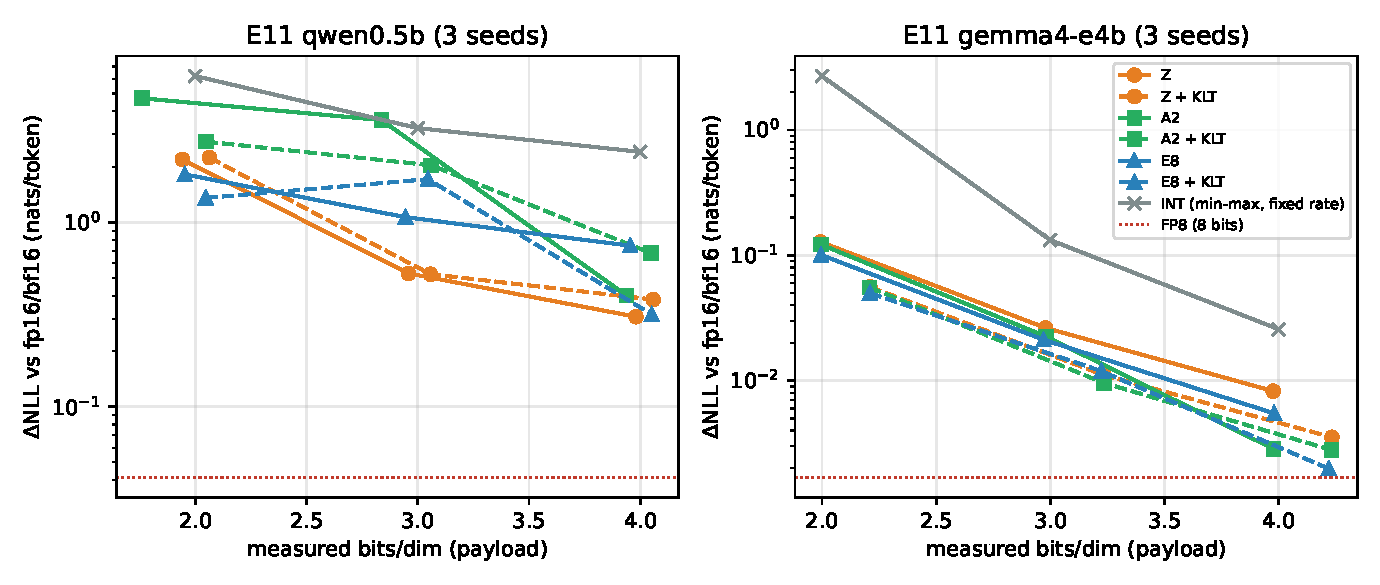
\includegraphics[width=\textwidth]{figures/fig8_e11_kv_lattice.pdf}
\caption{E11 on WikiText-2, three seeds per point. $\Delta$NLL (nats/token, log scale) against the measured payload rate (bits/dim) for $\mathbb{Z}$ (orange), $A_2$ per RoPE plane (green) and $E_8$ (blue), solid without and dashed with the per-head KLT, the INT min--max fixed-rate comparator (grey crosses) and the FP8 level (dotted red line). Left to right: Qwen2.5-0.5B-Instruct, Gemma-4-E4B (the invalid Qwen2.5-Coder-7B panel is withdrawn). Points whose measured rate misses the target by more than $0.1$ bit/dim are plotted at their realised rate and are not valid comparisons (Table~\ref{tab:e11_pairs}).}
\label{fig:e11}
\end{figure}

\textbf{Limitations.} (i) The scales were calibrated on two validation windows and did not always transfer to the test windows (Qwen-0.5B: $16$ of the 18 lattice cells are rate-matched). (ii) The quantisation is fake quantisation at prefill: each query attends to the quantised keys and values of all positions, which is what reading a quantised cache gives, but no fused kernel, no paged byte layout and no decode latency is measured. (iii) One dataset (WikiText-2). (iv) Sensitivity to KV quantisation differs by an order of magnitude between model families (FP8 $\Delta$NLL $+0.0413$ for Qwen-0.5B against $+0.0017$ nats for Gemma), so a result on one family does not transfer. (v) Three seeds are three window sets of one corpus, which gives low power and $df=2$ intervals.

\subsection{E12 pilot: does the spot-check replay survive a change of execution class?}
\label{sec:e12}

The external review of v3.5.0 objected that the Byzantine spot-check (replay one 50-step segment, accept iff $\|\theta_{\text{validator}}-\theta_{\text{worker}}\|_\infty \le 10^{-4}$) cannot survive hardware heterogeneity. E12 was pre-registered the same day (\texttt{artifacts/experiments/E12\_pilot\_prereg.json}) and run on the two CPU hosts available: this workstation (torch 2.14.0 CPU path, 4 threads) as the reference, and the Google Cloud TPU VM used in E8 (24-vCPU x86-64, torch 2.14.1+cpu, newer transformers and peft). The segment is the proof-of-concept configuration, \texttt{Qwen2.5-0.5B} with rank-8 LoRA on the query and value projections, AdamW, 50 steps of one 64-token window each, on 50 fixed windows of real text shipped with the harness so that both hosts see identical token ids; every cell starts from one saved initial adapter state. The statistic is the validator's own, $\ell_\infty$ over all 96 adapter tensors after step 50 (\texttt{artifacts/experiments/E12\_pilot\_report.json}).
\begin{itemize}[leftmargin=1.8em]
    \item \textbf{Controls.} A second run in a new process on the same host with the same thread count reproduces the adapters \emph{bit for bit} ($\ell_\infty = 0$, P12a supported). The tampered replay (sign of the adapter update flipped at step 25) ends at $1.3\cdot 10^{-3}$ with all 96 tensors above $\epsilon$ (positive control passed).
    \item \textbf{P12b (thread count only): refuted.} With 1 or 8 threads instead of 4, on the same host and build, the replay diverges from step 2 (loss differences of $10^{-6}$) and ends at $\mathbf{2.6\cdot 10^{-4}}$ and $2.5\cdot 10^{-4}$: above $\epsilon$, with 5 and 3 of the 96 tensors over threshold. Reduction order alone defeats the rule.
    \item \textbf{P12c (other host, other build): refuted as stated, and informative.} The TPU-VM replay ends at $\mathbf{1.5\cdot 10^{-4}}$ (4 of 96 tensors above $\epsilon$), also above $\epsilon$ but \emph{smaller} than the thread-count cells: the second host ran with 4 threads too, so the dominant source of divergence is the reduction order fixed by the thread pool, not the CPU model or the torch build.
    \item \textbf{P12d (bf16 autocast): supported, and worse than the tamper.} Running the forward pass in bfloat16 autocast on the same host, build and thread count (fp32 master adapter weights, replayed by an fp32 validator) diverges from step 0 and ends at $\mathbf{3.3\cdot 10^{-3}}$ with all 96 tensors above $\epsilon$ and a maximum loss difference of $1.7\cdot 10^{-2}$: $13\times$ the honest fp32 divergence and $2.7\times$ the tampered control. Neither the $\ell_\infty$ norm nor the tensor count can tell an honest bf16 worker from a tamperer when the validator replays in fp32, so dtype is a hard class boundary, not a tolerance. The cell took $5.3$\,h on CPU against $3$--$16$ minutes for the fp32 cells (a single-threaded bf16 path); the GPU bf16 class, which is the one the swarm will actually run, is measured in \texttt{HM-S10-08}.
\end{itemize}
Consequences. (i) The shipped rule accepts only bit-identical execution; it is re-specified in Section~4.1 as execution-class matched, with thread count and deterministic-kernel settings part of the class. (ii) The honest fp32 divergence after 50 steps on CPU is $1.5$--$2.6\cdot 10^{-4}$, and the one tampered run sat only $5\times$ above it in $\ell_\infty$; the count of tensors above threshold ($3$--$5$ vs.\ $96$) is the better discriminator and becomes the second term of the acceptance rule, with its false-rejection rate to be measured per class. Both terms saturate for an honest bf16 worker replayed in fp32 ($3.3\cdot 10^{-3}$, $96$ of $96$), so no per-class $\epsilon$ can admit a bf16 worker to an fp32 validator: validators are assigned within the dtype class, and the bf16 class gets its own $\epsilon$ from a GPU measurement before any bf16 worker is admitted (the pre-registered consequence of P12d). (iii) Nothing here is a GPU measurement: the T4 of this workstation is not reachable from Python and the RTX 2070 is on another machine, so the GPU classes that matter most for the swarm remain \texttt{HM-S10-08}.

\subsection{E12 on the T4: replay divergence of the spot-check across GPU and CPU classes (RQ11, \texttt{HM-S10-08})}
\label{sec:e12gpu}

E12 answers point W1 of the external review of v3.5.0 (\texttt{paper/review/}): is the $\epsilon = 10^{-4}$ replay rule of Section~\ref{sec:byz_replay_note} valid across heterogeneous accelerators? \textbf{Design.} The honest worker's segment and every validator replay are the repository's own \texttt{replay\_inner\_segment} (steps 0 to 50, AdamW at lr $2\cdot10^{-4}$, gradient clipping, micro-batch 1) on 64 WikiText-2 sequences of 128 tokens, with \texttt{Qwen2.5-0.5B-Instruct} in float32 on both devices and a hand-rolled rank-8 LoRA on \texttt{q\_proj}/\texttt{v\_proj} (PEFT is not installed on the host; $A\sim\mathcal{N}(0,1/r)$, $B=0$), the production determinism configuration being applied (no determinism warning was raised in any configuration). Each cell has $9$ segments (3 batch-order seeds $\times$ 3 initialisation seeds); the metric is $\|\theta_{\text{validator}}-\theta_{\text{worker}}\|_\infty$ over all LoRA tensors after 50 steps. Cells: (A) the T4 against itself in the same process (negative control, must be exactly $0$); (B) the T4 against the same T4 in a separate Python process (a proxy for ``same class''); (C) the T4 against this host's x86 CPU (cross class); (D) a named proxy that is \emph{not} a fixed-point kernel: both devices in float64 with the LoRA parameters snapped to a $2^{-20}$ grid after every optimiser step; (E) tamper (positive control): the worker flips the sign of one LoRA element after step 25 and an honest T4 replays. The experiment was pre-registered (\texttt{E12\_replay\_divergence\_prereg.json}).

\begin{table}[ht!]
\centering
\caption{E12: $\|\Delta\theta\|_\infty$ after 50 inner steps over 9 segments per cell; $\epsilon = 10^{-4}$.}
\label{tab:e12}
\vspace{0.35em}
\begin{tabular}{@{}lccc@{}}
\toprule
\textbf{Cell} & \textbf{Min} & \textbf{Max} & \textbf{Segments above $\epsilon$} \\
\midrule
A\;same process, T4 & $0.0$ & $0.0$ & $0/9$ \\
B\;separate process, T4 & $0.0$ & $0.0$ & $0/9$ \\
C\;T4 vs x86 CPU, float32 & $2.0\cdot10^{-4}$ & $6.3\cdot10^{-4}$ & $9/9$ \\
D\;proxy: float64 + $2^{-20}$ snapping, T4 vs CPU & $2.0\cdot10^{-4}$ & $6.3\cdot10^{-4}$ & $9/9$ \\
E\;tamper (positive control) & $2.6$ & $3.0$ & $9/9$ \\
\bottomrule
\end{tabular}
\end{table}

\textbf{Results and decisions.} Same-process and separate-process T4 divergence is exactly $0.0$ in all nine segments, so \textbf{P12-same is supported}: with the production determinism settings a GPU replay on the same device is bit-exact, and $\epsilon$ is not the binding quantity within a class. T4 against the x86 CPU gives $2.0\cdot10^{-4}$ to $6.3\cdot10^{-4}$, above $\epsilon$ in $9/9$ segments, so \textbf{P12-cross is supported}: an honest cross-class replay fails the rule. The divergence is already of the same order at step 10 as at step 50 (it does not build up over the segment). The fp64 + grid-snapping proxy does not reduce the cross-device divergence (same range), so it is no evidence that a cheap rounding discipline repairs the rule. Tamper gives $2.6$ to $3.0$, four orders of magnitude above the honest cross-class value, so the check separates tampering from architecture drift by a wide margin; both controls passed. \textbf{The fixed-point clause of P12 stays open}: it requires a true fixed-point attention kernel, which does not exist in this repository, and the proxy is not one. That the cross-device divergence is of the order of the inner learning rate from step 10 on is consistent with the sign-like early steps of Adam turning any tiny gradient difference into a step of about the learning rate; this is an interpretation, not a registered result.

\textbf{Consequence.} Validators are assigned by accelerator class (\texttt{src/hivemind/boinc/validator\_assignment.py}); a cross-class replay is reported as ``not comparable'' and never flags an account. This turns the architecture-matched rule of Section~\ref{sec:byz_replay_note} from a stated assumption into a measured necessity for the pair measured here.

\textbf{Limitations.} The RTX 2070 (another host), a TPU-VM CPU and a second T4 were \emph{not run}: ``same class'' is approximated by the same T4 in a separate process, which is weaker than two physical cards, and nothing is claimed for other GPUs. The LoRA initialisation $\mathcal{N}(0,1/r)$ is about $18\times$ the PEFT default scale and may inflate the cross-class magnitudes (the same initialisation made E10b diverge, above); one model, rank 8, 50 steps, float32.


\subsection{Status of the research program at v3.8.0}
\label{sec:status380}

Run and decided as registered on a single Tesla T4 on 23--24 October 2026: E10b (invalid, positive control failed in seed 3; descriptive distortion ratio only), E11 (P11a refuted on Qwen2.5-0.5B, on one rate-matched cell, and on Gemma-4-E4B, P11b refuted overall on the valid models; the Qwen2.5-Coder-7B row is invalid because its negative control failed and its verdicts are withdrawn; the KV ring stays on FP8) and E12 (P12-same and P12-cross supported). Still open: the RTX 2070, TPU-VM and second-T4 cells of E12; a true fixed-point replay kernel (the fp64 snapping proxy did not help); a longer E10b with enough rounds and larger deltas to resolve codec effects on the loss; a fused KV kernel and decode-latency measurement should a lattice page codec ever be reconsidered; and the E5 campaign at 0.5B scale. The swarm simulation E13 (with its exploratory replications E13c and E13d), the fairness follow-up E14, the coding-assistant experiment E15 and the E16 measurement of the GWAYA-Lite tiers have since been run on the same T4 and are reported in Sections~\ref{sec:e13}, \ref{sec:e14}, \ref{sec:e15} and~\ref{sec:e16} (E13: protocol exact, the registered all-on configuration refuted as viable at $K=\lceil M/2\rceil$; E14: supported on the dense model and inconclusive on the MoE; E15: H15a inconclusive, H15b and H15d supported; E16: H16a supported, H16d inconclusive on the 7B tier). What remains open after them: the multi-host WAN gameday \texttt{HM-S9-07} (no WAN, NAT, QUIC or volunteer-churn measurement exists; every swarm number in this paper comes from one host, thread-hosted except one two-process identity run); the RTX 2070 and TPU-VM cells (and the second T4) of E12; a true fixed-point replay kernel; a longer E10b; the E11b exploratory sweeps, which were not run; E13 with four real OS processes of the 0.5B model, which needs $20.03$\,GiB against $13.76$\,GiB free; and E14 on the WAN and with more seeds. As before, no peer review of record has taken place and no score is claimed: the provenance lock only certifies that the numbers of this section equal those of the receipts in \texttt{artifacts/experiments/}.

% === MARKER: add the E11b (exploratory sweep) and E13 (swarm simulation) subsections here ===

% ---------------------------------------------------------------------------
% v3.8.0 additions, second batch: E13 (swarm simulation on one GPU), E14 (fair quorum /
% deferred carry), E15 (GWAYA-gated rejection-sampling fine-tuning), E16 (GWAYA-Lite tiers
% on a T4) and the GWAYA-Lite deployment. Numbers are locked to the receipts by
% paper/autoevolve_peer_review_pipeline.py (PROV-52 onward).
% ---------------------------------------------------------------------------
\subsection{E13: a swarm simulation on one GPU (\texttt{HM-S9-07} precondition): the protocol is exact, the $K=\lceil M/2\rceil$ configuration is not viable at this size}
\label{sec:e13}

\textbf{Question and design.} E13 is the localhost negative control that the E8 design asks for before any multi-host measurement: do $M$ independent workers that exchange LoRA deltas over real localhost HTTP, with a minimum quorum $K<M$, the adaptive grace window, Radial-Directional Averaging (RDA), the $E_8$ lattice codec at 2 bits/dim with error feedback (``\texttt{E8@2+EF}''), a straggler and a churn event, reach a held-out loss close to a synchronous single-process DiLoCo run at matched tokens? Three models: the dense \texttt{Qwen2.5-0.5B-Instruct} (4 workers, domains code, French Wikipedia, PubMed, GSM8K) and two \emph{pretrained} mixture-of-experts models, \texttt{Granite-3.1-1B-A400M} (32 experts, top-8, 24 layers; 3 workers) and \texttt{Granite-3.1-3B-A800M} (40 experts, top-8, 32 layers; 4 workers). Rank-8 LoRA on \texttt{q\_proj}/\texttt{v\_proj} (PEFT-scale initialisation, the lesson of E10b), 6 rounds of 20 inner steps, AdamW inner and Nesterov outer (lr $0.7$), micro-batch $4\times256$ tokens, non-IID data (worker $i$ trains only on domain $i$), a fixed 16-sequence-per-domain held-out mixture. The workers' quorum, grace and RDA code is the repository's \texttt{decoupled\_diloco.py}. Cells: S0 synchronous single-process baseline; S1 the HTTP swarm with $K=M$, direct average, no codec (identity control); S2 all mechanisms on ($K=\lceil M/2\rceil$, adaptive grace, RDA, \texttt{E8@2+EF}, worker $M{-}1$ delayed by $2\times$ its median compute in rounds 1, 3, 5, worker 1 killed after round 2 and re-spawned with fresh optimizer and error-feedback state before round 4); S3, S4, S5 the each-mechanism-off variants (no codec, no RDA, $K=M$). Three seeds (one for the 3B model, which is a feasibility run). The experiment was pre-registered (\texttt{artifacts/experiments/E13\_swarm\_local\_prereg.json}) before any run, with six amendments, listed here because several of them change how the result must be read.

\textbf{Amendments and their reasons.} (1) After an adversarial code review by a separate model and before any real-model run: deterministic algorithms and math attention on the T4, a diagnostic twin S0b, evaluation versions $0/3/6$ only and by a rotating worker (the first build let the code-domain worker evaluate every version, which delayed it and disadvantaged its domain in the $K<M$ cells), stride-sampled held-out windows, hang protection, a memory preflight with a registered thread-hosting fallback, and \texttt{experts\_implementation=eager} for Granite on a reviewer's prediction. No prediction, margin or threshold was changed. (2) The preflight found that four OS processes of the 0.5B model need $20.03$\,GiB against $13.76$\,GiB free, so the registered 0.5B swarm cells run \emph{thread-hosted} (four peer threads over the same real HTTP protocol, one frozen model, peers' forward/backward serialised); a separate $M=2$ run with real OS processes was added. (3) The exploratory diagnostic E13c (below), written after the 0.5B result. (4) The first Granite-1B execution was aborted by the registered time fail-fast (measured $2.686$\,s per inner step, projected $3.09$\,h against a limit of $3$\,h), and a step benchmark (\texttt{E13\_granite\_step\_bench.json}) \emph{corrected amendment~1}: \texttt{grouped\_mm} runs at $0.78$\,s per step against $1.45$\,s for \texttt{eager} and $2.54$\,s for \texttt{eager} with gradient checkpointing, i.e.\ the reviewer's prediction was wrong on this stack; Granite-1B was rerun with \texttt{grouped\_mm}, thread-hosted ($5.76$\,GiB peak does not allow three processes), while the 3B run stays on \texttt{eager} (its seed-1 run is the registered feasibility run; the two implementations are not bit-comparable, so no further 3B seeds were run). (5) The $M=2$ OS-process run was aborted by the registered learning gate ($0.0253$ nats gained by round 3 against $0.05$); for that identity-only run the gate was relaxed to $0.0$, and it remains $0.05$ everywhere else. (6) The exploratory six-domain replication E13d (below). \textbf{Only the $M=2$ run used separate OS processes}; every other swarm cell, including all the registered ones, is thread-hosted. The transport is real HTTP on the loopback interface in every case.

\textbf{Controls.} S1 equals S0: the final LoRA vectors have $\max|\Delta| = 0.0$ (tolerance $10^{-6}$) for all three 0.5B seeds, all three Granite-1B seeds and the single Granite-3B seed, and the S0b twin is bit-identical to S0, so \textbf{P13a is supported} on every model, including thread-hosted peers, and in the $M=2$ run with two real OS processes ($\max|\Delta|=0.0$, one seed, no status assigned by the amendment). S0 learns (the mixture held-out loss falls from $2.365$ to between $2.231$ and $2.233$ on the 0.5B model), all workers start from the same initialisation (equal sha256), raw upload bodies are exactly $4\times$ the coordinate count, the measured codec rate is within $0.05$ bit/dim of $2.0$, and no cell failed; all controls registered for the three main models pass, so the run is valid. The reports of the two exploratory runs (E13c and $M=2$) carry \texttt{controls\_all\_passed: false}; this is not a failed control: the E13c grid has no S1 cell (identity and raw-wire controls) and the $M=2$ grid has no S2 cell (codec-rate control), and the report records \texttt{null}, not \texttt{false}, for the controls it did not evaluate.

\begin{table}[ht!]
\centering
\caption{E13 registered runs and the two exploratory replications ($\pm$ = 95\,\% half-width, $df=2$). $\rho$ is the registered retention $(L_{0}-L_{\mathrm{S2}})/(L_{0}-L_{\mathrm{S0}})$ per seed, the share of the synchronous baseline's held-out improvement that the all-on swarm keeps; the viability bar is $0.5$. ``S0 gain'' is the per-seed range of $L_0-L_{\mathrm{S0}}$ in nats. The upload ratio is the measured size of the S2 upload bodies over the raw fp32 delta bytes (ideal entropy-coded value $0.062$). Source receipts: \texttt{E13\_swarm\_local\_report*.json} and \texttt{E13\_swarm\_local\_predictions*.json}.}
\label{tab:e13}
\vspace{0.35em}
\resizebox{\textwidth}{!}{%
\begin{tabular}{@{}llcccccc@{}}
\toprule
\textbf{Run} & \textbf{$M$ / $K$ / seeds} & \textbf{S0 gain} & \textbf{S2 $-$ S0 final loss} & \textbf{Retention $\rho$} & \textbf{P13b} & \textbf{Upload ratio} \\
\midrule
Qwen2.5-0.5B (dense) & $4/2/3$ & $0.132$--$0.135$ & $+0.140 \pm 0.044$ & $-0.05 \pm 0.35$ & \textbf{refuted} & $0.091$ \\
Granite-1B-A400M (MoE) & $3/2/3$ & $0.051$--$0.057$ & $+0.090 \pm 0.022$ & $-0.66 \pm 0.66$ & \textbf{refuted} & $0.091$ \\
Granite-3B-A800M (MoE) & $4/2/1$ & $0.103$ & $+0.175$ (n=1) & $-0.70$ (n=1) & descriptive & $0.091$ \\
E13c rotating straggler (0.5B) & $4/2/3$ & $0.132$--$0.135$ & $+0.080 \pm 0.042$ & $0.40 \pm 0.30$ & exploratory & -- \\
E13d six domains (0.5B) & $6/3/3$ & $0.120$--$0.123$ & $+0.086 \pm 0.046$ & $0.29 \pm 0.39$ & inconclusive & $0.091$ \\
\bottomrule
\end{tabular}}
\end{table}

\textbf{Registered results.} \textbf{P13b (swarm viability, $\rho\ge0.5$ with a lower interval bound at or above $0.5$) is refuted on both models with three seeds}: on the dense model $\rho = -0.05 \pm 0.35$ (per seed $-0.15$, $-0.11$, $+0.11$), on Granite-1B $\rho = -0.66 \pm 0.66$ (per seed $-0.45$, $-0.56$, $-0.96$; the upper bound of the interval, $+0.006$, is below the bar). The all-on swarm finishes \emph{above its starting loss} in 5 of the 6 seed runs of the two models, i.e.\ it kept none of the synchronous improvement in the sense of the registered ratio. On Granite-3B (one seed, no interval, no status by the registered rule) the point value is $-0.70$. \textbf{P13c (wire cost) is supported} on all three models: the measured upload bodies (int8 codewords, scale, zlib; no int16 fallback was needed) are $9.1\,\%$ of the raw fp32 deltas against a bar of $30\,\%$ and an ideal entropy-coded ratio of $6.2\,\%$ at $2.0$ bits/dim, i.e.\ a measured $11.0\times$ reduction where the ideal is about $16\times$; the codec's measured rate was $1.99$ to $2.00$ bit/dim.

\begin{table}[ht!]
\centering
\caption{E13 P13d (descriptive, no status): each mechanism removed from the all-on cell, \texttt{Qwen2.5-0.5B}, $M=4$, three seeds. ``Late discards'' counts deltas that arrived outside the grace window, summed over the three seeds. The paired difference $L(\mathrm{S2})-L(\mathrm{S}x)$ is positive when removing the mechanism lowers the held-out loss.}
\label{tab:e13_mech}
\vspace{0.35em}
\resizebox{\textwidth}{!}{%
\begin{tabular}{@{}lccccc@{}}
\toprule
\textbf{Cell} & \textbf{Retention $\rho$} & \textbf{Final loss $-$ S0} & \textbf{$L(\mathrm{S2})-L(\mathrm{S}x)$} & \textbf{Admitted fraction} & \textbf{Late discards} \\
\midrule
S2 all on ($K=2$) & $-0.05$ & $+0.140 \pm 0.044$ & -- & $0.50$ & $27$ \\
S3 no codec & $0.11$ & $+0.118 \pm 0.034$ & $+0.022 \pm 0.078$ & $0.50$ & $25$ \\
S4 no RDA & $0.26$ & $+0.098 \pm 0.040$ & $+0.042 \pm 0.040$ & $0.50$ & $26$ \\
S5 no quorum ($K=M$) & $0.94$ & $+0.008 \pm 0.006$ & $+0.133 \pm 0.041$ & $0.96$ & $0$ \\
\bottomrule
\end{tabular}}
\end{table}

\textbf{What loses the learning (P13d).} Removing the codec or the RDA merge from the all-on cell leaves it near the all-on retention ($0.11$ and $0.26$), and removing the quorum, i.e.\ waiting for the straggler ($K=M$, admitted fraction $0.96$, the churned worker being dead for one round), keeps $0.94$ of the synchronous improvement and ends within $0.008 \pm 0.006$ nats of S0 (Table~\ref{tab:e13_mech}). On this evidence the $E_8$ codec costs little and the harm in S2 comes from the $K<M$ quorum with a persistent straggler that is always the same non-IID domain: about half of the deltas are discarded every round ($0.50$ admitted) and the GSM8K domain (worker $M{-}1$) is the one starved, its held-out loss ending at $1.60$ against $1.23$ for S0 (per-domain means over the three seeds). Two observations are less comfortable for the design. RDA does not help in this cell: the no-RDA cell has the \emph{lower} loss ($+0.042 \pm 0.040$, an interval that only just excludes zero), so the norm-restoring multiplier of Section~\ref{sec:decoupled} gives no benefit here; and the S3 contrast includes zero. Both statements are descriptive, from three seeds of one non-IID configuration whose straggler schedule is fixed.

\textbf{E13c: a rotating straggler (exploratory, Amendment~3).} Is the loss caused by one domain being starved, or by $K=2$ of $4$ itself? The straggler was rotated (worker 3 in round 1, worker 2 in round 3, worker 1 in round 5; everything else as S2). The hypothesis was recorded before the run and had no threshold. The retention, computed here with the registered formula from the report's final losses, is $0.40 \pm 0.30$ (per seed $0.53$, $0.29$, $0.38$) against $-0.05 \pm 0.35$ for the fixed straggler, with the final loss $+0.080 \pm 0.042$ above S0 instead of $+0.140 \pm 0.044$. Rotating the straggler recovers part of the loss and not all of it ($K=M$ keeps $0.94$), so domain starvation explains a part and $K=\lceil M/2\rceil$ itself the rest; the two intervals overlap and no test of that contrast was registered.

\textbf{E13d: six non-IID domains and $M=6$ (exploratory replication, Amendment~6).} Adding news (CNN/DailyMail) and fiction (LAMBADA) to the four domains, with $K=3$ for S2 and a persistent straggler on the fiction domain, the registered rules were applied unchanged and are reported as replication statuses: S1 equals S0 in all three seeds ($\max|\Delta|=0.0$), P13c is supported again (upload ratio $0.091$), and P13b is \textbf{inconclusive}: $\rho = 0.29 \pm 0.39$ (per seed $0.37$, $0.39$, $0.11$; interval $[-0.10, +0.68]$ straddles the bar). The no-quorum cell again keeps $0.94$ ($\rho = 0.94 \pm 0.07$) and ends $+0.007 \pm 0.008$ nats from S0, an interval that includes zero. The registered refutation on four domains therefore is not reproduced as a refutation with six, and it is not contradicted either; with three seeds the data do not decide between ``viable at $0.5$'' and ``not viable''.

\textbf{Mixture-of-experts routing (descriptive, no prediction).} Routing statistics were recorded from forward hooks on the routers of the final global model of S0, seed 1, on the held-out windows of each domain. Granite-1B: mean normalised routing entropy per layer $0.913$ (code), $0.929$ (French Wikipedia), $0.946$ (PubMed); share of tokens on the $25\,\%$ most-used experts $0.517$, $0.501$, $0.456$. Granite-3B: entropy $0.890$ (code), $0.916$ (French Wikipedia), $0.927$ (PubMed), $0.904$ (GSM8K); top-quartile share $0.583$, $0.529$, $0.504$, $0.557$. The domains are routed differently in degree (code is the most concentrated), but the entropies are all between $0.89$ and $0.95$ and these are per-domain marginals of a model whose routers and experts are frozen; they say nothing about expert specialisation, and E13 trains no experts.

\textbf{What E13 can and cannot claim.} It claims that the swarm protocol (quorum selection, adaptive grace, RDA, the $E_8$ codec with error feedback, churn, token-weighted merging over HTTP) is numerically exact against a synchronous run when nothing is dropped ($\max|\Delta|=0.0$, thread-hosted and, for $M=2$, with real processes), that the codec cuts upload bytes by the measured factor, and that in this testbed the registered all-on configuration does not keep the learning. It does \emph{not} claim anything about a WAN, NAT traversal, QUIC, volunteer churn, throughput or latency percentiles (all workers share one GPU and one host, round latencies are time-sharing artefacts and are not used), anything about hidden-state expert routing across machines, NF4, Skip-Token, Skip-Attention, PA-CGAD or fixed-point exits (none is in the cells), or anything about expert-level training (LoRA is on attention only; the Granite experts and routers are frozen but used in every forward pass).

\textbf{Consequence.} The pre-registered consequence of a refuted P13b applies: the all-on swarm at $K=\lceil M/2\rceil$ loses more than half of the synchronous improvement at this size, and the loss was attributed with P13d (the quorum) \emph{before} any WAN run; the exact protocol is a necessary precondition for the multi-host gameday \texttt{HM-S9-07}, not a substitute for it. E14 (next subsection) tests two admission policies against that finding.

\textbf{Limitations.} (i) Thread-hosted peers share one frozen model and serialise their forward/backward passes, which is not a swarm of processes; only $M=2$ used OS processes, and on one seed. (ii) Six rounds of twenty steps: the starting loss is far from converged and a larger gain from the baseline would change the denominator of the retention ratio; on Granite-1B the synchronous baseline improves the held-out loss by only $0.051$ to $0.057$ nats, so $\rho$ there is a ratio of small numbers. (iii) Three seeds resample the initialisation and the batch order and \emph{not} the straggler schedule, the shards or the process timing, so S2--S5 contain scheduling nondeterminism that the seeds do not sample; the Granite-3B result is one seed. (iv) The $0.5$ viability bar was chosen before any run and is not a power-based equivalence margin. (v) Granite-1B and Granite-3B used different expert implementations (Amendment~4); one pretrained-MoE family only.

\subsection{E14: a fair quorum and a deferred carry (exploratory follow-up of E13; \texttt{HM-S10-13}): supported on the dense model, inconclusive on the MoE}
\label{sec:e14}

E14 was written after the E13 result and the E13c diagnostic and before any run of the two mechanisms (\texttt{E14\_swarm\_fairness\_prereg.json}); it is exploratory and decides no registered E13 prediction. \textbf{S6 (fair quorum)} bounds the exclusion of a live worker: a worker excluded from \texttt{MAX\_EXCLUSION}$=1$ consecutive closed rounds must be in the next quorum; the round closes only after the $K$-quorum plus the grace window \emph{and} every such worker has posted (its delta is then admitted); dead workers never block; the extra wait is capped at $0.5\times$ the stall-watchdog limit, after which the round closes with what is present. \textbf{S7 (deferred carry)} queues a late or out-of-grace delta instead of discarding it and merges it into the next round as an extra arrival with weight $\text{token weight}/(1+s)$, $s$ being the staleness in versions; deltas with $s>$\,\texttt{MAX\_STALENESS}$=2$ are discarded; carried deltas count neither toward $K$ nor toward the grace window. The constants were fixed in advance and not tuned. Both cells are otherwise S2 ($K=\lceil M/2\rceil$, adaptive grace, RDA, \texttt{E8@2+EF}, the registered straggler and churn); S2 is re-run in the same invocation so that S2, S6 and S7 are paired seed by seed. Models and seeds: \texttt{Qwen2.5-0.5B} ($M=4$) and \texttt{Granite-3.1-1B-A400M} ($M=3$, \texttt{grouped\_mm}), three seeds, thread-hosted. Rules: H14a (S6 keeps more than S2) and H14b (S7 keeps more than S2) are decided on the per-seed paired difference $L(\mathrm{S2})-L(\mathrm{cell})$ with the $df=2$ interval (supported if above zero, refuted if below, inconclusive if it includes zero); the retention, round latency and carried-delta counts are descriptive; two hypotheses per model, no multiple-comparison correction. The hypothesis statuses below are computed from the reports by those rules.

\begin{table}[ht!]
\centering
\caption{E14 (three seeds, $\pm$ = 95\,\% half-width). Retention $\rho$ is relative to the synchronous baseline S0 of the same invocation; the viability bar is $0.5$. $L(\mathrm{S2})-L(\mathrm{cell})$ is positive when the mechanism lowers the held-out loss against S2. Round latency is the p50 over 18 rounds on a time-shared GPU (descriptive). Source receipts: \texttt{E14\_report\_qwen0.5b.json}, \texttt{E14\_report\_granite1b.json}.}
\label{tab:e14}
\vspace{0.35em}
\resizebox{\textwidth}{!}{%
\begin{tabular}{@{}llccccc@{}}
\toprule
\textbf{Model} & \textbf{Cell} & \textbf{Retention $\rho$} & \textbf{Final loss $-$ S0} & \textbf{$L(\mathrm{S2})-L(\mathrm{cell})$} & \textbf{Status} & \textbf{Round p50 (s)} \\
\midrule
Qwen2.5-0.5B & S2 (re-run) & $-0.05 \pm 0.35$ & $+0.140 \pm 0.044$ & -- & -- & $16.5$ \\
 & S6 fair quorum & $0.88 \pm 0.08$ & $+0.016 \pm 0.011$ & $+0.124 \pm 0.055$ & H14a supported & $21.0$ \\
 & S7 deferred carry & $0.53 \pm 0.18$ & $+0.063 \pm 0.025$ & $+0.077 \pm 0.066$ & H14b supported & $16.3$ \\
\midrule
Granite-1B-A400M & S2 (re-run) & $-0.37 \pm 0.36$ & $+0.075 \pm 0.018$ & -- & -- & $42.7$ \\
 & S6 fair quorum & $-0.08 \pm 0.17$ & $+0.059 \pm 0.008$ & $+0.016 \pm 0.025$ & H14a inconclusive & $50.4$ \\
 & S7 deferred carry & $-0.67 \pm 0.57$ & $+0.091 \pm 0.018$ & $-0.016 \pm 0.034$ & H14b inconclusive & $43.3$ \\
\bottomrule
\end{tabular}}
\end{table}

\textbf{Dense model.} On \texttt{Qwen2.5-0.5B} both hypotheses are \textbf{supported}: S6 keeps $0.88 \pm 0.08$ of the synchronous improvement (the all-on S2 keeps $-0.05 \pm 0.35$ and $K=M$ in E13 keeps $0.94$) and S7 keeps $0.53 \pm 0.18$ (the point value is above the $0.5$ bar, the interval includes it). The S2 re-run reproduces the registered E13 values exactly for all three seeds (final losses and hence the retention $-0.05 \pm 0.35$ are identical). The price of S6 is time: the p50 round latency rises from $16.5$\,s to $21.0$\,s (\textbf{$+27.5\,\%$}, a median over 18 rounds, GPU time-shared, so descriptive), through $79.2$\,s of extra waiting in total (in 10 of the 18 rounds) and $13$ forced admissions, with no fair-wait timeout; the admitted fraction rises from $0.50$ to $0.68$ and the late discards fall from $27$ to $20$. S7 costs no latency (p50 $16.3$\,s), carries $18$ late deltas (staleness 1 in $16$ cases and staleness 2 in $2$; none discarded as too stale; none left unmerged at the end) and cuts the late discards from $27$ to $6$.

\textbf{Mixture-of-experts model.} On \texttt{Granite-3.1-1B-A400M} neither effect is resolved: $L(\mathrm{S2})-L(\mathrm{S6}) = +0.016 \pm 0.025$ and $L(\mathrm{S2})-L(\mathrm{S7}) = -0.016 \pm 0.034$ (both inconclusive), and every retention (S2 $-0.37 \pm 0.36$, S6 $-0.08 \pm 0.17$, S7 $-0.67 \pm 0.57$) is below the bar. Two caveats weigh heavily. The synchronous baseline improves the held-out loss by only $0.051$ to $0.057$ nats per seed, so the retention is a ratio with a small, noisy denominator; and the S2 re-run does \emph{not} reproduce the registered E13 Granite-1B values (seed 1 is identical, seeds 2 and 3 are not: retention $-0.37$ in this invocation against $-0.66$ in E13 under the same design), the scheduling nondeterminism that the pre-registration flagged. The Qwen2.5-0.5B support therefore does not transfer clearly to the MoE at this size, and the reports' \texttt{controls\_all\_passed: false} reflects only that the E14 grid has no S1 cell (the identity control is \texttt{null}); the learning, codec-rate and no-failed-cell controls pass.

\textbf{Consequence.} Following the pre-registered consequence for a supported hypothesis on a model, S6 and S7 are recorded as a \emph{candidate} admission policy for the multi-host gameday and as roadmap item \texttt{HM-S10-13}; neither is adopted into the default syncer. They need the WAN, more seeds and a configuration where the baseline's gain is larger before any default is changed. The experiment cannot change the E13 verdicts; one GPU, thread-hosted peers, two models, three seeds, fixed constants (\texttt{MAX\_EXCLUSION}, \texttt{MAX\_STALENESS}) that were not tuned.

\begin{figure}[ht!]
\centering
\includegraphics[width=\textwidth]{figures/fig9_e13_e14_retention.pdf}
\caption{Retention $\rho$ of the synchronous baseline's held-out improvement (three seeds, error bars = 95\,\% half-width, $df=2$) for the cells of E13 (S2--S5), E13c (rotating straggler) and E14 (S6, S7). Left: \texttt{Qwen2.5-0.5B}, $M=4$. Right: \texttt{Granite-3.1-1B-A400M}, $M=3$ (E13 registered S2 and the E14 re-run S2 differ in seeds 2 and 3). Dotted line: the registered viability bar $0.5$; dashed line: the synchronous baseline ($\rho=1$). Hatching distinguishes the cells without colour.}
\label{fig:e13_e14}
\end{figure}

\subsection{E15: GWAYA-gated rejection-sampling fine-tuning of a coding assistant under an enforced 8\,GB budget (\texttt{HM-S10-11})}
\label{sec:e15}

\textbf{What GWAYA is here.} GWAYA (the author's \texttt{xaviercallens/GWAYA-GwenLayaOpenModel} repository, MIT) is a fail-closed verification layer: a candidate is accepted only if a zero-stub AST audit is clean \emph{and} an oracle (sandboxed execution of the task tests) passes, otherwise the verdict is \texttt{UNVERIFIED}. It trains nothing. E15 adds the training around it: the gate decides which model-generated solutions become training data and which inference-time candidate is returned. \textbf{Pipeline.} Only \texttt{ast\_audit.py} is used, vendored unmodified at the pinned commit \texttt{9c0001e8307d} (sha256 \texttt{af8f382c5a67\ldots}; \texttt{third\_party/gwaya/PROVENANCE.md}); the oracle is \emph{not} GWAYA's own Bubblewrap oracle (\texttt{bwrap} is not installed on the host) but our own user/mount/net/pid/ipc/uts-namespace sandbox with tmpfs over the home directory, dropped capabilities, resource limits and an empty environment, tested with hostile probes; it has no seccomp filter, shares the host kernel, and the verdict is therefore reported as ``GWAYA-style''. Model: \texttt{Qwen2.5-Coder-1.5B-Instruct} in fp16 with a hand-rolled rank-16 LoRA ($\alpha=32$, on \texttt{q,k,v,o,gate,up,down} of every layer; $18{,}464{,}768$ trainable parameters, fp32 optimizer states, fp16 autocast), with \texttt{torch.cuda.set\_per\_process\_memory\_fraction} set to $7.5$\,GiB at process start so that every stage runs inside an 8\,GB card budget although the T4 has 15\,GB. Data: MBPP full train and validation (464 problems; \textbf{462} after removing two whose normalised prompt text occurs in the evaluation set, Amendment~1) for rejection sampling and fine-tuning only; evaluation on MBPP-sanitized test ($n=257$, disjoint task ids) and on HumanEval ($n=164$, never trained on). The prompt contains the problem and the \emph{visible} test \texttt{test\_list[0]}; the inference-time gate sees only that test; the final pass@1 uses all tests. Conditions: C0 base, greedy; C1 base plus the GWAYA inference loop (greedy, then two samples at $T=0.7$, the first candidate that passes the audit and the visible test wins, else up to three repair rounds fed with the gate's feedback, else the first greedy reply); RFT generation of 8 samples per train problem ($T=0.8$), gate with all tests, at most 2 distinct accepted solutions kept; 3 epochs, lr $2\cdot10^{-4}$ cosine; C2 tuned, greedy; C3 tuned plus the loop; HumanEval for C0 and C2 only. The experiment was pre-registered (\texttt{E15\_gwaya\_rft\_prereg.json}) with one amendment before any real-model generation (the 462-problem set, the functional definition of pass@1 with the audit used for selection and not for the final judgement, the vendored auditor and sandbox details, the time fail-fast).

\begin{table}[ht!]
\centering
\caption{E15 results (one training run; paired McNemar tests, exact two-sided; ``gained/lost'' = problems solved only by the second/first condition). Wilson 95\,\% intervals. ``Gen. GPU s'' is the GPU time of the generation (C1 and C3 include the reused greedy generation of C0 and C2). Source receipt: \texttt{E15\_gwaya\_rft\_report.json}.}
\label{tab:e15}
\vspace{0.35em}
\resizebox{\textwidth}{!}{%
\begin{tabular}{@{}llccccc@{}}
\toprule
\textbf{Cond.} & \textbf{Benchmark} & \textbf{Passes / $n$} & \textbf{pass@1 \% (Wilson 95)} & \textbf{Paired contrast} & \textbf{Gained/lost, $p$} & \textbf{Gen. GPU s} \\
\midrule
C0 base, greedy & MBPP & $169/257$ & $65.8$ $[59.8, 71.3]$ & -- & -- & $228.2$ \\
C1 base + loop & MBPP & $187/257$ & $72.8$ $[67.0, 77.8]$ & C1$-$C0 $+7.0$ pts & $19/1$, $p=4.0$e$-05$ & $1001.2$ \\
C2 tuned, greedy & MBPP & $171/257$ & $66.5$ $[60.6, 72.0]$ & C2$-$C0 $+0.8$ pts & $15/13$, $p=0.85$ & $198.3$ \\
C3 tuned + loop & MBPP & $190/257$ & $73.9$ $[68.2, 78.9]$ & C3$-$C1 $+1.2$ pts & $12/9$, $p=0.66$ & $688.6$ \\
 & & & & C3$-$C0 $+8.2$ pts & $26/5$, $p=1.9$e$-04$ & \\
C0 base, greedy & HumanEval & $110/164$ & $67.1$ $[59.6, 73.8]$ & -- & -- & $253.6$ \\
C2 tuned, greedy & HumanEval & $111/164$ & $67.7$ $[60.2, 74.4]$ & C2$-$C0 $+0.6$ pts & $12/11$, $p=1.0$ & $186.1$ \\
\bottomrule
\end{tabular}}
\end{table}

\textbf{Controls and decisions.} All registered controls pass: the gate accepts $100/100$ MBPP reference solutions (bar $95\,\%$) and $164/164$ HumanEval canonical solutions (bar $98\,\%$), $12/12$ planted stubs are rejected, every hostile-candidate probe (secret read, network, memory bomb, infinite loop, fork bomb, disk fill, host process inspection, tampering with the vendored auditor) is contained, and there is no leakage (no shared task id or normalised prompt after the two removals; two identical reference solutions under different prompts remain and are reported). \textbf{H15a} (RFT lifts greedy pass@1 by at least $+3.0$ points with $p<0.05$) is \textbf{inconclusive}: $+0.8$ points, $p=0.85$ (and no harm: not refuted). \textbf{H15b} (the loop lifts the base by at least $+5.0$ points) is \textbf{supported}: $+7.0$ points, $19$ gained and $1$ lost, $p=4.0\cdot10^{-5}$. H15c (stacking, descriptive): C3 against C1 is $+1.2$ points ($p=0.66$) and C3 against C0 $+8.2$ points ($p=1.9\cdot10^{-4}$). H15e (transfer to HumanEval, descriptive): $+0.6$ points, $p=1.0$. \textbf{H15d} (every stage runs to completion under the $7.5$\,GiB cap) is \textbf{supported}: the largest peak reserved memory of any stage is $4.47$\,GiB (limit $8.0$\,GiB), with no out-of-memory retry in the generation of the evaluation stages. The rejection-sampling yield is $359$ of $462$ train problems with at least one accepted solution (mean per-sample yield $0.542$), $673$ kept pairs, $329{,}948$ generated tokens; the fine-tuning ran $129$ steps and the mean cross-entropy fell from $0.156$ to $0.096$ to $0.061$ over the three epochs.

\textbf{The honest reading.} The lift of the pipeline comes from selecting among candidates against the visible test, not from repair and not from training. C1 gains $19$ problems over C0 and loses one. When the greedy reply passes the audit and the visible test it is kept unchanged, so every gain comes from the two samples or from repair; repair rounds solved only $1$ of the $54$ problems that entered them ($53$ fell back to the greedy reply; $2$ of $53$ for the tuned model), so at least $18$ of the $19$ gains come from the samples. The visible test accepted $79.4\,\%$ of the problems with a verified candidate, while $72.8\,\%$ pass all tests: a selector that sees one test is a weaker oracle than the hidden ones. Training on the gated samples changed greedy accuracy by $+0.8$ points (not distinguishable from zero) at a cost of $3{,}957$\,s of sampling plus $368$\,s of training, $4{,}325$ GPU-seconds in all, and the tuned loop (C3) does not beat the untuned loop (C1) ($+1.2$ points, $p=0.66$). The consequence registered for this case applies: H15a is not supported and H15b is: the inference-time gate alone is the efficient path, and training would need more verified data.

\begin{table}[ht!]
\centering
\caption{E15 cost per stage (whole-GPU NVML power $\times$ time, which includes any other process on the GPU: descriptive). The inference loop costs $4.4\times$ the GPU seconds of greedy decoding ($1001.2/228.2$, C1 including the reused greedy generation) and $3.9\times$ the generated tokens ($74{,}808$ against $19{,}285$). Source receipt: \texttt{E15\_gwaya\_rft\_report.json}.}
\label{tab:e15_cost}
\vspace{0.35em}
\begin{tabular}{@{}lccc@{}}
\toprule
\textbf{Stage} & \textbf{Wall (s)} & \textbf{Peak reserved (GiB)} & \textbf{Energy (Wh)} \\
\midrule
Baseline (C0, C0h) & $495.5$ & $4.18$ & $9.10$ \\
Base + loop (C1) & $800.8$ & $4.24$ & $14.66$ \\
RFT generation & $4046.7$ & $4.47$ & $74.80$ \\
Training (LoRA) & $368.1$ & $4.15$ & $6.72$ \\
Tuned (C2, C2h, C3) & $903.9$ & $4.36$ & $16.57$ \\
\bottomrule
\end{tabular}
\end{table}

\textbf{Limitations.} One fine-tuning run (no interval over training seeds; the paired tests do not contain training variance), one 1.5B model, MBPP-sanitized $n=257$ and HumanEval $n=164$, Python function synthesis only. The sampling seeds derive from the (task, sample) keys of each batch, so results depend on batch composition. The sandbox is not GWAYA's oracle and is a defence for a small model generating Python functions, not for adversarial third-party code. The vendored upstream auditor flags any \texttt{pass} outside an except handler or class body and any annotated \texttt{return None}-only function, so it can reject legitimate code; this lowers the RFT yield and was not tuned. No monetary or token reward is attached to the experiment.

\subsection{E16: GWAYA-Lite on a Tesla T4 (the measurement requested by GWAYA draft PR \#21) and the deployed assistant}
\label{sec:e16}

\textbf{Protocol.} GWAYA draft PR \#21 lists a T4 measurement of quantised coding tiers as blocked on a free T4; its text was treated as a specification to measure, not as instructions. E16 (\texttt{E16\_gwaya\_lite\_t4\_prereg.json}, pre-registered before the run) serves \texttt{qwen2.5-coder} 1.5B, 3B and 7B-instruct in the Q4\_K\_M format through Ollama $0.34.1$ (file sizes $940/1841/4466$\,MiB against $1070/1840/4466$\,MiB in the PR's tier table) on the T4. \emph{Resources:} for each tier and each \texttt{num\_ctx} in $\{4096, 8192\}$, GPU memory after load and after a prompt filling about $85\,\%$ of the context (the \texttt{nvidia-smi} delta over the idle baseline, CUDA context included), compared with the PR's estimator (weights $+$ KV per token $\times$ context $+ 600$\,MiB), decode and prompt-evaluation tokens per second (median over 12 fixed MBPP prompts, greedy). \emph{Accuracy:} MBPP-sanitized ($n=257$), same prompts, visible/hidden split and gate as E15; R = raw greedy, L = the GWAYA loop; the context-invariance check runs R again at 8192 for the 7B. \emph{Gate calibration (P2):} precision of the \texttt{VERIFIED} verdict (audit clean and visible test passed) against the hidden tests. \emph{Escalation ladder (descriptive):} 1.5B loop, then 3B loop on failure, then 7B loop, against the 7B loop alone, evaluated offline from the per-problem logs. Controls: idle GPU at start ($0$\,MiB used, bar $1500$), the gate control ($100/100$ references), $100\,\%$ of every tier on the GPU at both contexts (no CPU offload), every model unloaded at the end with the GPU back at $0$\,MiB (tolerance $300$), probes run one at a time without contamination, and a determinism repeat (10 problems generated twice greedily: $10/10$ identical for each tier). The run is valid.

\begin{table}[ht!]
\centering
\caption{E16 measured resources on a Tesla T4 (Ollama $0.34.1$, Q4\_K\_M, 100\,\% on the GPU in every row). VRAM is the \texttt{nvidia-smi} memory-used delta over the idle baseline, CUDA context included; the estimate is the PR \#21 formula; ``ratio'' is measured over estimate. Source receipt: \texttt{E16\_gwaya\_lite\_t4\_report.json} (the same numbers appear in the generated block of \texttt{docs/community/GWAYA\_T4\_DEPLOYMENT.md}).}
\label{tab:e16_vram}
\vspace{0.35em}
\resizebox{\textwidth}{!}{%
\begin{tabular}{@{}llccccc@{}}
\toprule
\textbf{Tier} & \textbf{num\_ctx} & \textbf{VRAM (MiB)} & \textbf{PR estimate (MiB)} & \textbf{Ratio} & \textbf{Decode tok/s} & \textbf{Prompt-eval tok/s} \\
\midrule
1.5B & 4096 & 1651 & 1782 & 0.93 & 130.5 & 2841 \\
1.5B & 8192 & 2107 & 1894 & 1.11 & 127.9 & 2769 \\
3B & 4096 & 2713 & 2584 & 1.05 & 68.3 & 1541 \\
3B & 8192 & 3297 & 2728 & 1.21 & 67.1 & 1580 \\
7B & 4096 & 5483 & 5290 & 1.04 & 28.5 & 812 \\
7B & 8192 & 6387 & 5514 & 1.16 & 28.2 & 827 \\
\bottomrule
\end{tabular}}
\end{table}

\begin{table}[ht!]
\centering
\caption{E16 MBPP-sanitized pass@1 at \texttt{num\_ctx} 4096 ($n=257$): raw greedy R against the GWAYA loop L, paired exact McNemar (gained/lost = solved only by L / only by R), and the precision of \texttt{VERIFIED} verdicts against the hidden tests (Wilson 95\,\%). The ladder row is the descriptive small-first cascade.}
\label{tab:e16_acc}
\vspace{0.35em}
\resizebox{\textwidth}{!}{%
\begin{tabular}{@{}lcccccc@{}}
\toprule
\textbf{Tier} & \textbf{R pass@1 \%} & \textbf{L pass@1 \%} & \textbf{L $-$ R (pts)} & \textbf{Gained/lost} & \textbf{McNemar $p$} & \textbf{Precision of \texttt{VERIFIED} \%} \\
\midrule
1.5B & 64.6 ($166$) & 73.2 ($188$) & $+8.6$ & $22/0$ & 4.8e-07 & 92.6 [88.2, 95.5] \\
3B & 72.8 ($187$) & 80.2 ($206$) & $+7.4$ & $19/0$ & 3.8e-06 & 92.8 [88.6, 95.5] \\
7B & 81.7 ($210$) & 85.6 ($220$) & $+3.9$ & $10/0$ & 2.0e-03 & 94.8 [91.2, 97.0] \\
Ladder 1.5B$\to$3B$\to$7B & -- & 85.2 ($219$) & -- & -- & -- & -- \\
\bottomrule
\end{tabular}}
\end{table}

\textbf{Registered statuses.} \textbf{H16a} (the 7B tier fits in $6656$\,MiB, the PR's accept criterion) is \textbf{supported} at 4096 ($5483$\,MiB) and at 8192 ($6387$\,MiB, a margin of $269$\,MiB); the $6656$\,MiB ceiling is a Windows WDDM reserve for an 8\,GB card and this host is Linux with the full 15\,GB available, so it is tested here as a threshold and not as a physical limit. \textbf{H16b} (the PR's estimator is within a factor $[0.80, 1.25]$ of the measurement for every tier and context) is \textbf{adequate}: the ratios range from $0.93$ to $1.21$ (the 3B at 8192 is $1.21$, close to the edge: the estimator under-states the context-dependent part). \textbf{H16c} (the loop does not lower pass@1) is supported on all three tiers, with no problem lost to the loop in any tier. \textbf{H16d} (the loop lifts pass@1 by at least $+5.0$ points with $p<0.05$) is \textbf{supported for the 1.5B ($+8.6$) and the 3B ($+7.4$) and inconclusive for the 7B}: the 7B gain, $+3.9$ points with $p=0.002$, is statistically clear but below the registered $+5.0$ bar. \textbf{H16e} (precision of \texttt{VERIFIED} at least $0.80$, so that the word is justified) is \textbf{supported}: $92.6\,\%$, $92.8\,\%$ and $94.8\,\%$ for the three tiers; $5$ to $7\,\%$ of the \texttt{VERIFIED} solutions still fail the hidden tests, and no hidden-test-passing candidate was rejected by the gate. \textbf{H16f} (descriptive, interactive bar of $20$ tok/s for the 7B decode at 4096) is met at $28.5$\,tok/s.

\textbf{The escalation ladder (descriptive, no status).} The small-first cascade reaches $85.2\,\%$ ($219/257$) against $85.6\,\%$ ($220/257$) for the 7B loop alone (paired: $8$ gained, $9$ lost, $p=1.0$), escalating $21.0\,\%$ of the problems to the 3B and $12.1\,\%$ to the 7B, at $78\,\%$ of the 7B-only model time ($1227$\,s against $1566$\,s). The PR's worry that small tiers might cost more than going straight to the 7B is therefore not borne out on this benchmark: the cascade is statistically indistinguishable in accuracy and cheaper in model time. \textbf{Context invariance.} The 7B raw run at 8192 solves exactly the same $210$ problems as at 4096 ($0$ discordant, $p=1.0$), which is expected since the prompts are far below $1.5$k tokens. Where the loop's winners come from: for the 1.5B, the greedy reply wins for $178$ problems, the first or second sample for $15+10$, and $54$ problems fall back to the first greedy reply after three repair rounds; for the 7B the corresponding counts are $219$, $9+4$ and $25$, with no repair success: again the selection among candidates, not repair, carries the lift. A descriptive comparison with E15: the raw 1.5B at Q4\_K\_M, $64.6\,\%$, and the fp16 base of E15, $65.8\,\%$, are close (different runtimes, quantisation and sampling paths; no test was registered).

\textbf{The deployment.} \texttt{scripts/gwaya\_lite.py} is the deployable form of the measurement: a small-first ladder (1.5B, then 3B, then 7B, Q4\_K\_M via the local Ollama daemon) behind the E15 gate, with three subcommands (\texttt{ask}, \texttt{serve}, \texttt{doctor}), CPU-testable with a fake Ollama and the real sandbox. Verdict wording is strict: \texttt{VERIFIED} only when the audit is clean and \emph{the user's} tests pass in the sandbox; \texttt{AUDITED} when the request carried no tests (never reported as verified); \texttt{UNVERIFIED} when the sandbox cannot be established (fail-closed); \texttt{FAILED} otherwise. The OpenAI-compatible gateway on \texttt{127.0.0.1:8099} listens on the loopback interface only, refuses a non-loopback bind unless an API-key file is given as well, rejects requests with a foreign \texttt{Host} or \texttt{Origin} header, caps request sizes, serialises requests (one GPU job at a time), enforces a maximum resident-GPU budget and unloads the models on exit. The live-check receipt (\texttt{artifacts/gwaya\_lite\_live\_check.json}) records, on the deployed service: health and model list answered; $3/3$ tasks \texttt{VERIFIED} (two by the 1.5B tier, and one, \texttt{fizzbuzz}, after the ladder escalated to the 3B tier through 7 candidates and 3 repair rounds); a request without tests answered \texttt{AUDITED} and never \texttt{VERIFIED}; an SSE stream of $13$ data chunks ended by the terminator; foreign \texttt{Host} and \texttt{Origin} answered 403; and $1639$\,MiB of GPU memory in use after the requests, with only the 1.5B model resident. The service has not been tested in a real editor, and its gate is the one of E15, not GWAYA's Bubblewrap oracle.

\begin{figure}[ht!]
\centering
\includegraphics[width=\textwidth]{figures/fig10_e16_gwaya_lite_tiers.pdf}
\caption{E16 on a Tesla T4. Left: measured VRAM (MiB) per Q4\_K\_M tier at \texttt{num\_ctx} 4096 and 8192, with the PR \#21 estimate (black markers) and the $6656$\,MiB threshold of H16a (dotted line). Right: MBPP-sanitized pass@1 (\%) for the raw greedy model (R) and the GWAYA loop (L) per tier and for the small-first ladder (L only), with Wilson 95\,\% intervals.}
\label{fig:e16}
\end{figure}

\textbf{Limits of E16.} One runtime (Ollama), one quantisation (Q4\_K\_M), one benchmark (MBPP-sanitized, $n=257$, Python only), one seed set; greedy decoding is not guaranteed bit-stable (the determinism repeat found $10/10$ identical, which is evidence and not a guarantee); a Linux host, not the Windows/WDDM environment for which the PR's ceiling was written; a sandbox that is not GWAYA's own. The PR's Qwen3.5 and TPU tiers are not measured. The publication of these results on the GWAYA repository or its PR is left to the repository's owner. As for every result in this paper, the lock certifies only that the numbers of these subsections equal those of the receipts.




\subsection{Directions drawn from the author's other publications and repositories}
\label{sec:directions}

HiveMind is one project of a larger body of work, and the review of 23 October 2026 asked which of the author's published results can be \emph{used} here rather than cited. Four can, each with a definite next artifact.
\begin{enumerate}[leftmargin=1.8em]
    \item \textbf{Method.} The protocol of Section~\ref{sec:research} (pre-registration, positive/negative/matched-random controls, a claim ledger, a kernel-checked formal layer, numbers entering the text only through a provenance lock) is the laboratory method of~\cite{callens2026labmethod}, with the autoresearch screening loop of~\cite{callens2026autoresearch} as the intended search procedure for the 0.5B-scale E5 sweep; the pre-registration-then-ledger-gate harness that E5-het and E10 follow is the one built for OptimalEnergyAI~\cite{callens2026triangular}.
    \item \textbf{Lattice codecs, twice over.} The $E_8$ decoders of E10 are the same family used for the ``Gosset $E_8$ dicodon quantisation'' of~\cite{callens2026genetics}; a single shared package with the two-sided decoder check as its test suite is the obvious refactor (\texttt{HM-S10-07}).
    \item \textbf{KV-cache compression for the inference ring (E11).} HiveMind's \texttt{FP8PagedKVCache} stores keys and values at 8 bits with per-page scales. Two measured results suggest a better codec: the RunuX study of PolarQuant on a commodity GPU~\cite{callens2026runuxkv}, and OptimalEnergyAI's finding that the hexagonal lattice $A_2$ applied per RoPE plane beats scalar quantisation by $22$--$36\,\%$ of $\Delta$NLL on \texttt{Qwen2.5-0.5B} keys without any transform, while $E_8$ needs a per-head decorrelating transform first~\cite{callens2026triangular}. E11 (pre-registration to be written before any run) compares FP8, $A_2$ per RoPE plane and $E_8$ at matched measured bits on real \texttt{Qwen2.5-0.5B} KV tensors, with the transform as a factor; its positive control is 2-bit scalar quantisation, which must hurt, and its negative control is 8-bit $A_2$, which must match FP8. Decision rule: a codec enters the inference ring only if it beats FP8 at equal bytes with the seed interval excluding zero. \emph{Update (v3.8.0): E11 was pre-registered and run on three models (the plan above with \texttt{Qwen2.5-Coder-7B-Instruct} and \texttt{Gemma-4-E4B} added); the Coder-7B row is invalid (its negative control failed) and withdrawn; P11a was refuted on Qwen2.5-0.5B (on one rate-matched cell) and on Gemma and no lattice codec was adopted, see Section~\ref{sec:e11}.}
    \item \textbf{A real workload.} The 8-domain campaign that E5 at scale needs has so far used synthetic tasks; the Laya-LoRA curriculum of ten structured coding datasets~\cite{callens2026laya} is a real LoRA workload with a published evaluation, and \texttt{HM-S10-06} asks whether it can be the campaign's data without changing what E5 measures.
\end{enumerate}
What is deliberately \emph{not} leveraged: the commercial RunuX runtime code (its 1-bit compressor was re-implemented from~\cite{bernstein2018signsgd}), and the kernel, string-theory and number-theory formalisations, which share method but no mechanism with this system.

% ============================================================================
\section{Limitations, Threats to Validity, and Future Multi-Host Benchmarks}
\label{sec:limitations}
% ============================================================================

\textbf{What this paper establishes vs.\ what remains open.}
\begin{enumerate}[leftmargin=1.8em]
    \item \textbf{Single-host process simulation vs.\ multi-host WAN deployment.} While Experiments E1--E4 validate held-out generalization across synchronization regimes, PA-CGAD straggler resilience, fixed-point halting trade-offs, and subspace spectra in controlled PyTorch runs, all workers to date have executed on a single physical host. Real residential WAN packet loss, NAT hole-punching failure rates, and cross-vendor GPU floating-point drift remain to be measured over a live multi-node deployment.
    \item \textbf{Single seed in E1--E4.} Every experiment in Section~\ref{sec:exp_eval} uses one seed (2026) and therefore demonstrates that the mechanisms behave as specified without estimating an effect size. E5-toy (Section~\ref{sec:e5toy}), E5-het (Section~\ref{sec:e5het}) and the E8 pilot (Section~\ref{sec:e8pilot}) are the first three-seed, controlled measurements; the IID toy's main finding is that it is too easy to rank the mechanisms.
    \item \textbf{Full-scale standard benchmark suites.} While Experiment E1 evaluates held-out cross-entropy and perplexity on a 128-sequence disjoint validation split, full zero-shot/few-shot evaluations on standard LLM benchmarks (full GSM8K test split, HumanEval pass@1, PubMedQA) for 0.5B--7B upcycled MoE checkpoints are still required.
    \item \textbf{128-expert training scale.} The largest MoE trained end-to-end on the RTX 2070 has 4 experts (96 FFN modules). The 3-tier 128-expert hierarchical router, FoMoE partial replication, and Skip-Attention prefetching have been verified at the module/planner level (\texttt{H3}, \texttt{H5}, \texttt{E4}) but not yet trained across 128 domain branches.
    \item \textbf{Adaptive Byzantine adversaries.} Our Multi-Krum + $2\sigma$ cosine filter has been verified against sign-flipped/scaled poisoners; subtle inner-product manipulation (ALIE) and coordinated Sybil coalitions under non-IID drift warrant dedicated red-team evaluation.
    \item \textbf{Spot-checks across execution classes.} The $\epsilon = 10^{-4}$ replay rule of Section~4.1 fails on CPU for a thread-count change alone (E12 pilot, $2.6\cdot 10^{-4}$); it holds only for bit-identical execution. The bf16 precision class, replayed in fp32, diverges by $3.3\cdot 10^{-3}$ with every tensor above threshold, more than the tampered control: dtype is a class boundary that no tolerance crosses. GPU classes and the false-rejection rate of the tensor-count statistic are not yet measured (\texttt{HM-S10-08}); until they are, the Byzantine pillar's acceptance rule is an execution-class-matched claim with a per-class $\epsilon$ still to be set. \emph{Update (v3.8.0): the T4 was measured (Section~\ref{sec:e12gpu}); the rule holds exactly within one T4 (separate process) and fails between a T4 and an x86 CPU, so the same-class claim is now a measured requirement for that pair. RTX 2070, TPU and second-T4 cells remain unmeasured.}
    \item \textbf{Open after the October 2026 T4 campaign.} E10b gave no valid loss result at 0.5B scale (six rounds of twenty steps cannot resolve codec effects; Section~\ref{sec:e10b}); E11 rests on fake quantisation at prefill, one dataset, three window-set ``seeds'', a single rate-matched cell for the $A_2$ comparison on Qwen-0.5B, and an invalid Qwen2.5-Coder-7B row (negative control failed) whose FP8 arm has not been investigated (Section~\ref{sec:e11}); E12 compares a T4 with its own separate process and one x86 CPU only, with a LoRA initialisation about $18\times$ larger than the PEFT default (Section~\ref{sec:e12gpu}). A true fixed-point replay kernel, the RTX 2070 and TPU cells and a longer E10b remain to be done. The E13 swarm simulation has since been run and is reported in Sections~\ref{sec:e13} to~\ref{sec:e16}.
    \item \textbf{Compounding approximations.} NF4 base weights, 2-bit DCT outer gradients with error feedback, Skip-Token, speculative Skip-Attention, PA-CGAD truncation and fixed-point loop exits were each verified in isolation (H1--H11, E1--E4). Their interaction under WAN churn has not been measured; E8's design therefore includes an all-mechanisms-on cell against each-mechanism-off cells so that an interaction, and not only main effects, can be detected. Representation collapse under compounded noise is a live threat to validity, not a solved one.
    \item \textbf{Proof-of-concept scale.} The RTX 2070 run trains on 8 rows per worker; its loss curves are memorisation. It establishes the VRAM budget and the end-to-end plumbing and nothing about learning quality.
    \item \textbf{Scope of Lean 4 formalization.} The 128 Lean 4 lemmas in \texttt{lean4/HiveMindSpec.lean} verify discrete arithmetic, hypothesis-necessity counterexamples, non-vacuity inhabitation, and byte-budget invariants over $\mathbb{N}$/$\mathbb{Z}$ (Section~2); they do not formalize real-valued stochastic convergence or C++/CUDA kernel equivalence. A compiling lemma is not automatically a constraint on the system: Theorems 125 and 127 of Season 15 compile under the axiom whitelist yet say nothing about the gate or the barrier they are named after (one conjunct is a tautology, one hypothesis is unused). They stay in the count because the count is a count of compiled declarations; the inventory table marks them.
    \item \textbf{No peer review of record has taken place.} An external review of v3.5.0 whose author is not stated was received on 23 October 2026; it is recorded verbatim with a point-by-point response in \texttt{paper/review/} and led to the revisions of v3.6.0, but it is not a peer review of record. \texttt{paper/autoevolve\_peer\_review\_pipeline.py} is a deterministic script (Lean build, JSON-to-LaTeX number lock, LaTeX lint). Versions 2.9--3.1 of this preprint and its \texttt{PEER\_REVIEW\_REPORT.json} labelled that script a ``Claude Opus 5.5 / Gemini 5-round peer review'' with referee scores of 9.4--9.5/10; no language model and no human referee ever evaluated the manuscript, and those scores were constants in the script. The labels and scores are removed in v3.2.0 and the report now states \texttt{is\_peer\_review: false}. Several entries of \texttt{docs/ACKNOWLEDGMENTS\_AND\_CITATIONS.md} and \texttt{CITATION.cff} also carried invented titles, authors or arXiv identifiers; they were re-verified against arXiv on 23 October 2026 and corrected or removed, and every entry of this paper's bibliography was checked individually.
\end{enumerate}

\subsection{Epistemic Stratification \& 6-Layer Security/Hardness Attestation}

To prevent conflating machine-checked discrete arithmetic with empirical single-host measurements or unvalidated multi-host WAN scaling, Table~\ref{tab:epistemic_matrix} stratifies all claims into three explicit verification tiers. Concurrently, the repository is audited by the 6-Layer \texttt{HiveMindHardnessEngine} (\texttt{results/hivemind\_hardness\_report.json}), verifying: (L1) zero AST stubs across all modules; (L2) zero security findings across $147$ scanned repository files (\texttt{risk\_score = 0}); (L3) $25/25$ simulated Byzantine, Sybil, NaN-injection, and WDDM TDR attack vectors blocked; (L4) $120/120$ Lean 4 theorems compiled with $0$ \texttt{sorry} and $0$ custom axioms; (L5) exact rational bridge verification (\texttt{NF4} $128/33$, \texttt{DiLoCo} wire $5000/3$, \texttt{Prefix-Trie} $19/25$, \texttt{3-Tier MoE} $1/8$); and (L6) SHA-256 execution attestation.

\begin{table}[ht!]
\centering
\footnotesize
\caption{Epistemic stratification matrix separating machine-checked discrete lemmas, single-host empirical measurements, and open multi-host WAN validation targets.}
\label{tab:epistemic_matrix}
\vspace{0.35em}
\resizebox{\textwidth}{!}{%
\begin{tabular}{@{}llp{6.2cm}p{4.6cm}@{}}
\toprule
\textbf{Verification Category} & \textbf{Artifact / Proof Source} & \textbf{What Is Rigorously Established} & \textbf{Explicit Boundary / Not Claimed} \\
\midrule
\textbf{Category I: Lean 4 Kernel Lemmas} & \texttt{lean4/HiveMindSpec.lean} (120 lemmas, 0 \texttt{sorry}) & Discrete $\mathbb{N}/\mathbb{Z}$ byte budgets, flat-bucket partitions, EF21 telescoping sums, necessity counterexamples (Thms.\ 113--115), and \texttt{Nonempty} witness (Thm.\ 116). & Does not prove real-valued stochastic convergence or Python/CUDA kernel refinement. \\
\textbf{Category II: Controlled Empirical \& Single-GPU PoC} & \texttt{H1}--\texttt{H10}, \texttt{E1}--\texttt{E4}, RTX 2070 PoC (\texttt{artifacts/*.json}) & $0.052\%$ held-out loss gap at $12.49\times$ wire savings (\texttt{E1}); $11.6\times$ lower straggler MSE under PA-CGAD (\texttt{E2}); $1{,}509.5\text{\,MB}$ peak VRAM on 8\,GB RTX 2070; $25/25$ red-team vectors blocked. & Executed on a single physical host with synthetic WAN delays and controlled corpus shards. \\
\textbf{Category III: Open Multi-Host WAN Targets} & Future multi-node testbed (Section~\ref{sec:limitations}) & Analytical communication models for FoMoE ($3.46\times$) and Kademlia Geo-Ring topologies. & Live multi-host residential WAN throughput, NAT punch success rates, and 128-branch full GSM8K/HumanEval accuracy remain open. \\
\bottomrule
\end{tabular}%
}
\end{table}

\textbf{Reproducibility.} Every number and figure in this paper is generated deterministically from committed scripts and JSON artifacts:
\begin{itemize}[leftmargin=1.8em]
    \item \texttt{PYTHONPATH=src python -m hivemind.swarm.architecture\_hypothesis\_verifier} $\to$ \texttt{artifacts/architecture\_hypothesis\_verification\_report.json} (\texttt{H1}--\texttt{H10}, \texttt{pytest tests/test\_architecture\_hypotheses.py}).
    \item \texttt{PYTHONPATH=src python scripts/run\_paper\_experiments\_and\_figures.py} $\to$ \texttt{artifacts/paper\_v3\_experiments\_report.json} (\texttt{E1}--\texttt{E4}) and \texttt{paper/figures/fig1..fig4.\{pdf,png\}}.
    \item \texttt{PYTHONPATH=src python scripts/verify\_decoupled\_diloco\_quorum.py} $\to$ \texttt{artifacts/decoupled\_diloco\_quorum\_check.json} (\texttt{H11}, \texttt{pytest tests/test\_decoupled\_diloco\_quorum.py tests/test\_fomoe\_sigma\_routing.py}).
    \item \texttt{PYTHONPATH=src python paper/autoevolve\_peer\_review\_pipeline.py} $\to$ \texttt{paper/PEER\_REVIEW\_REPORT.json} (scripted static audit: Lean inventory, JSON-to-LaTeX provenance lock, LaTeX lint; it calls no language model and is not a peer review).
    \item \texttt{cd lean4 \&\& lake build} $\to$ compiles all 128 theorems in \texttt{lean4/HiveMindSpec.lean} with zero \texttt{sorry}.
    \item The PDF, the LaTeX source, the Lean specification and every JSON artifact quoted above are deposited on Zenodo under DOI \zenodoDOI{} (\texttt{scripts/publish\_hivemind\_paper\_zenodo.py}, receipt \texttt{paper/ZENODO\_DEPOSIT\_RECEIPT.json} with per-file MD5 verification).
\end{itemize}

\begin{thebibliography}{99}
\footnotesize
\bibitem{anderson2002boinc} D.~P. Anderson, ``BOINC: A System for Public-Resource Computing and Storage,'' in \textit{Proc. IEEE/ACM Int. Workshop on Grid Computing}, 2004, pp.~4--10.
\bibitem{douillard2023diloco} A.~Douillard, Q.~Feng, A.~A. Rusu, R.~Chhaparia, Y.~Donchev, A.~Kuncoro, M.~Ranzato, A.~Szlam, and J.~Shen, ``DiLoCo: Distributed Low-Communication Training of Language Models,'' \textit{arXiv:2311.08105}, 2023.
\bibitem{liu2024asynclocalsgd} B.~Liu, R.~Chhaparia, A.~Douillard, S.~Kale, A.~A. Rusu, J.~Shen, A.~Szlam, and M.~Ranzato, ``Asynchronous Local-SGD Training for Language Modeling,'' \textit{arXiv:2401.09135}, 2024. Code: \url{https://github.com/google-deepmind/asyncdiloco}.
\bibitem{douillard2025streamingdiloco} A.~Douillard, Y.~Donchev, J.~K. Rush, S.~Kale, Z.~Charles, G.~Teston, Z.~Garrett, J.~Shen, R.~McIlroy, D.~Lacey, A.~Ram\'e, A.~Szlam, M.~Ranzato, and P.~R. Barham, ``Streaming DiLoCo with Overlapping Communication: Towards a Distributed Free Lunch,'' in \textit{Second Conference on Language Modeling (COLM)}, 2025, \textit{arXiv:2501.18512}.
\bibitem{douillard2026decoupled} Decoupled DiLoCo Team (Google DeepMind \& Google Research; A.~Douillard, K.~Rush, Y.~Donchev, Z.~Charles, A.~Dubey, B.~Woodworth, \textit{et al.}), ``Decoupled DiLoCo for Resilient Distributed Pre-training,'' \textit{arXiv:2604.21428}, 2026.
\bibitem{callens2026labmethod} X.~Callens, ``A laboratory method for AI-assisted science: formal proof, exact arithmetic, controlled experiment, and a claim ledger, tested for a month on the Navier--Stokes problem,'' Zenodo, v1.10.2, 2026, doi:10.5281/zenodo.22829767.
\bibitem{callens2026autoresearch} X.~Callens, ``Karpathy-autoresearch Screening and Machine-Checked Elenchus Deep-Dive Across Fermat's Last Theorem, Navier--Stokes Admissibility Censorship, and Kinetic Spectral Caps: A Ten-to-Five Hypothesis Investigation in Lean 4,'' Zenodo, 2026, doi:10.5281/zenodo.23467992.
\bibitem{callens2026runuxkv} X.~Callens, ``RunuX: Deterministic Fixed-Point Attention and Measured PolarQuant KV-Cache Compression on a Commodity GPU, with a Hardware Test of Its TPU Claims,'' Zenodo, v2.0.0, 2026, doi:10.5281/zenodo.22879667.
\bibitem{callens2026genetics} X.~Callens, ``Non-Equilibrium Hopfield--Ninio Proofreading, Chimeric ART-Exo Fidelity, Gosset $E_8$ Dicodon Quantization, and Topological DNA Supercoiling in LeanFlow, rusty-SUNDIALS, and Lean 4,'' Zenodo, v3, 2026, doi:10.5281/zenodo.23526783.
\bibitem{callens2026laya} X.~Callens, ``Laya-LoRA Coding Companion: Asymmetric Dual-Process Test-Time Compute, Full-Scale Curriculum on 10 Structured Coding Datasets, and Serverless Multi-Tier Inference Infrastructure on GCP,'' Zenodo, 2026, doi:10.5281/zenodo.23095224.
\bibitem{conway1982fast} J.~H.~Conway and N.~J.~A.~Sloane, ``Fast Quantizing and Decoding Algorithms for Lattice Quantizers and Codes,'' \textit{IEEE Trans.\ Inf.\ Theory}, 28(2):227--232, 1982.
\bibitem{callens2026triangular} X.~Callens, ``The Triangular Lattice and Universal Optimality: human proofs, Lean 4 verification, numerical validation in Python and Rust, and physics from fluids to plasmas,'' Zenodo, 2026, doi:10.5281/zenodo.23295142; companion code \textit{OptimalEnergyAI} (\texttt{oai\_ml.core.quantise}, \texttt{oai\_ml.core.rate}).
\bibitem{bernstein2018signsgd} J.~Bernstein, Y.-X.~Wang, K.~Azizzadenesheli, and A.~Anandkumar, ``signSGD: Compressed Optimisation for Non-Convex Problems,'' in \textit{ICML}, 2018, \textit{arXiv:1802.04434}.
\bibitem{kale2025eager} S.~Kale, A.~Douillard, and Y.~Donchev, ``Eager Updates for Overlapped Communication and Computation in DiLoCo,'' \textit{arXiv:2502.12996}, 2025.
\bibitem{defazio2025gpa} A.~Defazio, K.~Mishchenko, P.~Raman, H.-J.~M.~Shi, and L.~Xiao, ``Smoothing DiLoCo with Primal Averaging for Faster Training of LLMs,'' \textit{arXiv:2512.17131}, 2025.
\bibitem{charles2025scalingdiloco} Z.~Charles, G.~Teston, L.~Dery, K.~Rush, N.~Fallen, Z.~Garrett, A.~Szlam, and A.~Douillard, ``Communication-Efficient Language Model Training Scales Reliably and Robustly: Scaling Laws for DiLoCo,'' \textit{arXiv:2503.09799}, 2025.
\bibitem{jaghouar2024opendiloco} S.~Jaghouar, J.~M. Ong, and J.~Hagemann, ``OpenDiLoCo: An Open-Source Framework for Globally Distributed Low-Communication Training,'' \textit{arXiv:2407.07852}, 2024. Code: \url{https://github.com/PrimeIntellect-ai/OpenDiLoCo}, \url{https://github.com/PrimeIntellect-ai/prime-diloco}.
\bibitem{sukhbaatar2024btm} S.~Sukhbaatar \textit{et al.}, ``Branch-Train-MiX: Mixing Expert LLMs into a Mixture-of-Experts LLM,'' \textit{arXiv:2403.07816}, 2024.
\bibitem{dettmers2023qlora} T.~Dettmers, A.~Pagnoni, A.~Holtzman, and L.~Zettlemoyer, ``QLoRA: Efficient Finetuning of Quantized LLMs,'' in \textit{NeurIPS}, 2023.
\bibitem{sani2026fomoe} L.~Sani, Z.~Cao, M.~Kurmanji, A.~Iacob, A.~Jovanovi\'c, Y.~Gao, W.~Zhao, and N.~D. Lane, ``FoMoE: Breaking the Full-Replica Barrier with a Federation of MoEs,'' \textit{arXiv:2606.19025}, 2026.
\bibitem{merolla2025fomoe} P.~Merolla, ``fomoe: Fast Opportunistic Mixture-Of-Experts,'' software repository, \url{https://github.com/pmerolla/fomoe}.
\bibitem{loopedmoe2026} Huang \textit{et al.}, ``Towards Looped Models Done Right. Part I: Topology, Input Injection, Recurrent-State Design,'' \textit{arXiv:2610.23036}, 2026.
\bibitem{loopedfp2026} Huang, Shi, Chen \textit{et al.}, ``Towards Looped Models Done Right, Part II: Rethinking at Fixed Points,'' \textit{arXiv:2610.06833}, 2026.
\bibitem{shah2026cgad} V.~Shah and J.~Sun, ``Cosine-Gated Adam-Decay: Drop-In Staleness-Aware Outer Optimization for Decoupled DiLoCo,'' \textit{arXiv:2605.09126}, 2026.
\bibitem{marczak2025iso} D.~Marczak, S.~Magistri, S.~Cygert, B.~Twardowski, A.~D. Bagdanov, and J.~van~de~Weijer, ``No Task Left Behind: Isotropic Model Merging with Common and Task-Specific Subspaces,'' in \textit{ICML}, 2025, \textit{arXiv:2502.04959}.
\bibitem{horoi2026isoloco} S.~Horoi, B.~Th\'erien, G.~Wolf, and E.~Belilovsky, ``Can Model Merging Improve Aggregation in DiLoCo?,'' \textit{arXiv:2607.03011}, 2026.
\bibitem{gargiulo2024tsv} A.~A. Gargiulo \textit{et al.}, ``Task Singular Vectors: Reducing Task Interference in Model Merging,'' in \textit{CVPR}, 2025, \textit{arXiv:2412.00081}.
\bibitem{peng2024demo} B.~Peng, J.~Quesnelle, and D.~P. Kingma, ``DeMo: Decoupled Momentum Optimization,'' \textit{arXiv:2411.19870}, 2024. Code: \url{https://github.com/bloc97/DeMo}.
\bibitem{sarfi2025sparseloco} A.~Sarfi, B.~Th\'erien, J.~Lidin, and E.~Belilovsky, ``Communication Efficient LLM Pre-training with SparseLoCo,'' \textit{arXiv:2508.15706}, 2025. Code: \url{https://github.com/one-covenant/SparseLoCo}.
\bibitem{miahi2026pulseloco} E.~Miahi and E.~Belilovsky, ``Understanding and Exploiting Weight Update Sparsity for Communication-Efficient Distributed RL,'' \textit{arXiv:2602.03839}, 2026.
\bibitem{asif2026heloco} Asif \textit{et al.}, ``HeLoCo: Efficient Asynchronous Low-Communication Training under Data and Device Heterogeneity,'' \textit{arXiv:2606.00271}, 2026.
\bibitem{twelftree2026wadiloco} M.~Twelftree, D.~Lemphers, A.~He, and Y.~Yang, ``Not Every Sync Is Safe: Calibrated DiLoCo Scheduling for Shared AI Infrastructure,'' \textit{arXiv:2607.02544}, 2026.
\bibitem{koneputugodage2026factoredgossip} C.~H. Koneputugodage, T.~Ajanthan, S.~Ramasinghe, H.~M. Dolatabadi, S.~Siriwardhana, G.~Avraham, V.~Shevchenko, K.~Pajak, J.~Snewin, and A.~Long, ``Factored Gossip DiLoCo: Reducing Blocking Communication in DiLoCo,'' \textit{arXiv:2606.22768}, 2026.
\bibitem{cagnasso2026gasloc} P.~Cagnasso, E.~Belilovsky, and E.~Oyallon, ``Unifying Local Communications and Local Updates for LLM Pretraining,'' \textit{arXiv:2606.11081}, 2026.
\bibitem{topollai2026restart} K.~Topollai, A.~Ma, T.~Dimlioglu, S.~J. Tay, and A.~Choromanska, ``Outer-Momentum Restarting in High-Dimensional Two-Phase Optimization,'' \textit{arXiv:2605.28585}, 2026.
\bibitem{agarwala2026twophase} A.~Agarwala, ``High dimensional theory of two-phase optimizers,'' \textit{arXiv:2603.26954}, 2026.
\bibitem{palanciyan2026crossfacility} Z.~Palanciyan, T.~van Osch, D.~van der Wal, O.~Kotevska, and T.~Kok, ``Cross-Facility LLM Pre-training on HPC: Elastic Aggregation, Data Leasing, and Queue-Aware Placement,'' \textit{arXiv:2610.03457}, 2026.
\bibitem{he2026autoloco} He \textit{et al.}, ``AutoLoCo: Communication Efficient Distributed LLM Training via Adaptive Synchronization,'' \textit{arXiv:2609.36662}, 2026.
\bibitem{jordan2024muon} K.~Jordan \textit{et al.}, ``Muon: An Optimizer for Hidden Layers in Neural Networks,'' technical blog post, 2024.
\bibitem{therien2025muloco} B.~Th\'erien, X.~Huang, A.~Defazio, I.~Rish, and E.~Belilovsky, ``MuLoCo: Muon is a Practical Inner Optimizer for DiLoCo,'' \textit{arXiv:2505.23725}, 2025.
\bibitem{belilovsky2026inner} E.~Belilovsky, S.~Horoi, E.~Oyallon, and B.~Th\'erien, ``How Inner Optimizers Shape Replica Scaling,'' \textit{arXiv:2610.19064}, 2026.
\bibitem{richtarik2021ef21} P.~Richt\'arik, I.~Sokolov, and I.~Fatkhullin, ``EF21: A New, Simpler, Theoretically Better, and Practically Faster Error Feedback,'' in \textit{NeurIPS}, 2021, \textit{arXiv:2106.05203}.
\bibitem{ryabinin2020hivemind} M.~Ryabinin and A.~Gusev, ``Towards Crowdsourced Training of Large Neural Networks using Decentralized Mixture-of-Experts,'' in \textit{NeurIPS}, 2020, \textit{arXiv:2002.04013}. Code: \url{https://github.com/learning-at-home/hivemind}.
\bibitem{borzunov2023petals} A.~Borzunov \textit{et al.}, ``Petals: Collaborative Inference and Fine-Tuning of Large Models,'' in \textit{Proc. ACL System Demonstrations}, 2023.
\bibitem{blanchard2017krum} P.~Blanchard, E.~M. El~Mhamdi, R.~Guerraoui, and J.~Stainer, ``Machine Learning with Adversaries: Byzantine Tolerant Gradient Descent,'' in \textit{NeurIPS}, 2017.
\bibitem{fedus2022switch} W.~Fedus, B.~Zoph, and N.~Shazeer, ``Switch Transformers: Scaling to Trillion Parameter Models with Simple and Efficient Sparsity,'' \textit{JMLR}, vol.~23, no.~120, pp.~1--39, 2022.
\bibitem{moura2021lean4} L.~de~Moura and S.~Ullrich, ``The Lean 4 Theorem Prover and Programming Language,'' in \textit{Proc. CADE-28}, 2021, pp.~625--635.
\end{thebibliography}

\end{document}
